\documentclass[12pt]{mythesis}

 % \makeglossaries
 % % \loadglsentries{glossaries_entries}
 % %%% A
 % %%% C
 % %%% D
 % %%% E
 % \newglossaryentry{EHV}{name=EHV, description={Extremely High Velocity}}
 % %%% F
 % \newglossaryentry{FoV}{name=FoV, description={Field-of-View}}
 % \newglossaryentry{FWHM}{name=FWHM, description={Full-Width Half-Maximum}}
 % %%% G
 % \newglossaryentry{GMCs}{name=GMCs, description={Giant Molecular Clouds}}
 % %%% H
 % \newglossaryentry{HST}{name=HST, description={Hubble Space Telescope}}
 % %%% I
 % \newglossaryentry{IHV}{name=IHV, description={Intermediate High Velocity}}
 % %%% K
 % %%% L
 % %%% M
 % %%% N
 % %%% O
 % %%% P
 % %%% Q
 % %%% R
 % \newglossaryentry{RA}{name=RA, description={Right Ascension}}
 % %%% S
 % \newglossaryentry{S/N}{name=S/N, description={signal-to-noise ratio}}
 % \newglossaryentry{SHV}{name=SHV, description={Standard High Velocity}}
 % %%% T
 % %%% U
 % %%% Y
 % \newglossaryentry{YSO}{name=YSO, description={Young Stellar Object}}
 % %%% Z


\title{The Title of your PhD Thesis about the Molecular Outflow of SVS~13}
\author{Guillermo Blázquez Calero}
\date{\today}
\institution{%
 Instituto de Astrofísica de Andalucia (IAA-CSIC)\\
 \vspace{0.5cm}
 Prog6ama de Doctorado en Física y Matemáticas (FisyMat)\\
 Universidad de Granada\\
}
\advisor{%
 {\large\bf Dr. Guillem Anglada}\\
 \vspace{0.25cm}
 {\large\bf Dra. Mayra Osorio}\\
}
\logo{%
  
\includegraphics[width=.47\linewidth]{images/LogosIAA_SO_BN.png}
  
\includegraphics[width=.47\linewidth]{images/UGR-MARCA-02-monocromo.png}
}

\begin{document}
\frontmatter %Use lowercase Roman numerals for page numbers
\maketitle
%\restoregeometry
\cleardoublepage

\chapter*{Acknowledgements}

Agradecimientos

\chapter*{Resumen}

Resumen de la tesis

\chapter*{Summary}

Summary of the thesis

\tableofcontents


\mainmatter % Now Use Arabic numerals for page numbers
\chapter{Introduction}

% The star formation process is intrinsically associated with a powerful ejection activity. Highly collimated (and partially ionized) jets with typical velocities of several hundred \kms\ are launched from the close vicinity of the protostar while conical molecular outflows with velocities on the order of $\sim$10~\kms\ are ubiquitously observed in CO and other molecules at mm wavelengths. The latter are believed to consist mainly of swept-up ambient material, and to regulate the final stellar mass and the star formation efficiency on cloud scales. Yet, their primary driving agent remains debated. In this thesis, we \dots. Our goal is to \dots


% \section{Star formation overview}
\section{The formation of stars}
% Scheme:\\
% Review of the star formation process.
% \citep[Review]{shuadamslizano1987}
% \citep[Review]{mckee2007} 
% \citep[Review on physics of star formation]{larson2003}
% % \citep[Review on high-mass star formation]{zinnecker2007}
% % \citep[Review on high-mass star formation]{tan2014}
% \citep[Notes on star formation]{krumholz2015}
% \citep[Review]{andre2014}
% % \citep[Review]{li2014}
% % Low-mass star formation.
% \hrule

In this section we review our current understanding of the process by which gas turns into solar-like stars.
% In this section we overview our knowledge on the process of how gas turns into a solar-like star.
% Stars are the fundamental objects of astronomy; thus, the formation of stars constitutes one of the basic problems of astrophyscs.
% Star formation: How gas turns into stars
% Stars are the atoms of the universe, and the problem of how stars form is at the nexus of much of contemporary astrophysics. By transforming gas into stars, star formation determinies the structure and evolution of galaxies. By tapping the nuclear energy in the gas left over from the Big Bang, it determines the luminosity of galaaxies and, quite possibly, leads to the reionization of the Univers. Most of the element -including those that make up the world around us- are formed in stars. Finally, the process of star formation is inextricably tied up with the formation and early evolution of planetary systems (Mckee2007)
% While there has long been theoretical speculation concerning the early life of stars, teh subject first became an empirical one iin the middle of the last century. *It was not until the middle of the last century, when the problem of the formation of a start became an empirical one.* Starting in the 1940s, the T Tauri class of objects, residing within dark clouds, was recognized and subsequently examined in considerable detail. This interest stemmed from the gradual realization that these peculiar variables represent a primitive phase of solar-type stars. It also became apparent that the observed objects must have condensed out of the dark clouds in which they are presently still found.  By the mid 1950s, theorists began constructing numerical models for the pre-main-sequence evolutionary phase. The following decade saw advances in understanding the basic physics of cloud collapse. Stahler and Palla 2004.
% By the 1980s, star formation became one of the most vigorous areas of astronomical research. Stahler and Palla 2004.

% \subsection{Gravitational collapse of a molecular cloud}
\subsection{The birthplaces of stars: From molecular clouds to dense cores}
% \subsection{Birthplaces of stars}.

%It is well stablished that 
% In the Galaxy and all spiral galaxies, molecular clouds are the sites of star formation hennebell2012
% (with temperatures only of several 10s K)
% Stahler Palla Table 3.1, p.71, T = 10-50 K
% (several 10s K)
% and densest
% where most of the gas is in molecular form.
% The mass of molecluar clouds 
% are composed by a mixture of molecular gas (mostly H$_2$) and small fraction ($1\%$ of its mass) by dust grains. 
% Stars are formed in molecular clouds\ldots
% Molecular clouds are the sites of star formation.
% Stars form through the gravitational collaps of cold interstellar clouds

Stars are formed within molecular clouds, which are the coldest ($T\simeq$10-30~K) and the densest ($n\simeq$ 10$^2$-10$^5$~\cmcu) regions of the interstellar medium (ISM), composed by a mixture of molecular gas and dust. The molecular gas is responsible of about 99 percent of the total mass of the molecular cloud, and its predominantly composed of H$_2$. Since H$_2$ molecules are not capable of emitting at low temperatures, other molecules are used as a proxy for H$_2$; most importantly, CO, but also other bright molecules as HCN, HCO+, CS, or HNC. The remaining $\sim 1$ percent of the mass of molecular clouds is attributed to dust grains, which are responsible of the high extinction at optical wavelengths; for this reason, molecular clouds in the solar neighbourhood ($\lesssim$500~pc) that are seen in silhouette against the background Galactic starlight are called ``dark clouds'' \citep{bergin2007}. Without the presence of dust, molecular clouds would cease to exist, as it protects the molecules from being dissociated by the interestellar UV radiation.
% Dust, however, and molecular clouds are intimately related. Without dust most star forming molecular clouds would cease to exist since the dust protects the molecules against dissociating interstellar uv radiation (uv radiation if effectively blocked once the optical extinction AV ≥1 and most clouds have AV values measured in tens to a few hundred magnitudes). (Jets_from_young_stars2007)

% Solar neighborhood = 500pc (stahler2004, henshaw2023)

% ; they are less abundant (by a factor of $\gtrsim$10$^{4}$), but have transitions excitable under the physical conditions of molecular clouds.
%(by a factor of $\gtrsim$10$^{4}$)
% Although most of its molecular gas content is H$_2$, high temperatures 
% %($\sim$ 500-1000~K)
% are required to excite it, so they are not found in states capable of emitting, so other molecules such as CO, H$_2$O, NH$_3$, CS, or HCN, easier to excite are used as tracers.
% % molecular clouds are too cold the excitation temperature of the lowest-lying transitions are too high. to observe its rotational transitions ($\sim$500-1000~K). 
% Thus, other molecules such as CO, H$_2$O, NH$_3$, CS, or HCN, are used as proxy to trace H$_2$; they are less abundant 
% %(by a factor of $\gtrsim$10$^{4}$)
% , but have transitions excitable under the physical conditions of molecular clouds. Also
% Moving past H2 , the next-brightest molecular line (not counting isotopologues of CO, which are generally found under the same conditions) in most galaxies is HCN. Other bright molecules are HCO+ , CS, and HNC, but we will focus on HCN as a synecdoche for all of these tracers. Like CO, the HCN molecule has rotational transitions that can be excited at low temperatures, and is abundant because it combines some of the most abundant elements. Thus the data set for correlations of HCN with star formation is the second- largest after CO (krumholtz 2017).
% The lowest-lying transition of H$_2$ is very weak, and it is 510~K above the ground state.  In a molecular cloud there are simply no H2 moleclues in states capable of emitting. The reason such a high temperature required to excite the H2 molecule is its low mass: for a quantum oscillator or rotor, the level spacing varies with reduced mass as m^{-1/2}. Thus the levels of H2 are much farther apart than the levelsof other diatomic moleclues (e.g., CO, O2, N2). It is the low mass o the hydrogen atom that creates our problems.
%, which are of rotational type,
% is extremely weak and occurs at 510~$K$. 
% A diatomic molecules as H$_2$ has three types of excitation: electronic (corresponding to excitations of one or more of the electrons), vibrational (corresponding to vibrational motion of the two nuclei), and rotational (corresponding to rotation of the two nuclei about the center of mass). Genereally electronic excitations are highest in energy scale, vibrational are next, and rotational are the lowest in energy.

% While the atomic gas fills much of the Galactic disk up to its nominal scale height, the molecular component occupies only about one percent of the available volume (stahler2004).
Molecular clouds occupy a small fraction of the volume of the ISM in the Galaxy. Their sizes range from 
%a few parsecs to 
$\sim$2-100~pc,
% and their masses from thousands to millions
with masses $\sim$10$^2$-10$^6~M_\odot$ \citep{williams2000, stahler2004, bergin2007, mckee2007, hennebelle2012}. 
In the Milky Way, it is estimated that 80 percent of the molecular hydrogen is found in the largest (10-100~pc) and most massive ($\sim$10$^4$-10$^6$~$M_\odot$) molecular clouds called Giant Molecular Clouds (GMCs), where most of the star formation take place \citep{dobbs2014, chevance2023}.
%Other molecular clouds up to a few tens of pc and with a few hundreds of solar masses are considered Small Molecular Clouds (SMCs).
% GMC contains most of the galactic H2, and are the loci of most star formation \citep{mckee}
% Within the Milky Way, over 80 percent of the molecular hydrogen resides in giant cloud clomplexes (Stahler & Palla)
% In the Milky Way, it is estimated that 80 percent of the molecular hydrogen is found in the largest and most massive molecular clouds, called Giant Molecular Clouds (GMCs), where most of the star formation take place. They have sizes of tens of pc, masses of $\sim 10^4$ - $10^6~M_\odot$, and typical mean densities of 100~cm$^{-3}$ \citep{dobbs2014, chevance2023}. 
Some prototypical examples of GMCs found in the Galaxy are Orion or Perseus clouds.
%, while examples of SMCs are the Taurus-Auriga or Ophiuchus clouds.
% The internal structure of GMCs is shaped by gravitation, turbulence and propagating shocks, magnetic fields, heating and cooling, and chemestry; many of these effects derive from stellar feedback.

The internal structure of GMCs presents a complex network of clumps and filaments, the latter being a characteristic of self-gravitating turbulent gas \citep{andre2014}. It is estimated that $\sim15$ percent of the total mass of molecular clouds are in the form of filamentary structures, whereas filaments host the $\sim$60-90 percent of the dense (column densities N(H$_2$)$>7\times10^{21}$~\cmsq) gas mass \citep{pineda2023}.
% MAGNETIC FIELDS ARE IMPORTANT!
% Written by you: Gravitation, turbulence, and magnetic fields shape the the internal structure of GMCs, which show a complex network of clumps and filaments, the latter being a characteristic of self-gravitating turbulent gas \citep{andre2014}. 
%frequently showing clumps and filaments,
% the latter being common in self-gravitating turbulent gas (André et al. 2014).
% Magnetic fields are important in substructure formation,
% through both MHD turbulence and the direction of large- scale flows, and have a role in stabilizing filaments and in directing accretion of material onto filaments and hubs, as well as providing direction to the collapse of cores \citep{pattle2023}. 
They are present in a very wide range of sizes of 0.1-100~pc and masses of 1-10$^5$~M$_\odot$, and show a self-similar hierarchical structure; i.e., filaments may break down into smaller and smaller filaments \citep{vazquez-semadeni2019,hacar2023}. % More references of observations are needed
% Both observations and simulations show that 
Filaments are not in equilibrium and are highly dynamical, with accretion flows onto and along them, playing and important role in funneling the gas from the extended cloud to the clumpy overdensities where the physical conditions for the formation of a star are met \citep[e.g.][]{gomez2014}. 

Filaments may fragment into prestellar cores, gravitationally bound dense clouds with typical sizes of $0.03$-$0.2$~pc, densities of 10$^4$-$10^5$ cm$^{-3}$, and masses of $0.5$-$5$~M$_\odot$, which are 
%associated to 
% the prestellar cores
 the precursors
of single low-mass ($M_*<8~M_\odot$) stars or simple stellar systems. 
The most massive substrutures in GMCs, the so-called ridges (high-density filaments, with $n>10^5$~M$_\odot$ over $\sim5$~pc$^3$) and hubs (parsec-size central clumps with several hundreds of M$_\odot$ fed by filaments), are associated with the progenitors of star clusters and high-mass ($M_*>8~M_\odot$) stars \citep{motte2018}. As an example, in Fig.~\ref{fig:NGC1333ridge} we show a column density map of the NGC~1333 ridge, which is associted to a young proto-cluster where low-mass stars are forming \citep{hacar2017}.
%Filaments fragment into gravitationally bound regions with sizes of $0.03$ - $0.2$~pc, densities of 10$^4$ - $10^5$ cm$^3$, and masses of $0.5$ - $5$ M$_\odot$, are the prestellar cores, the precursors of single stars or simple stellar systems.
%On average, ∼15percent of the total mass of molecular clouds is observed to be in the form of molecular filaments, while up to ∼60–90percent of the dense gas mass (defined as the mass of gas with column density NH2 > 7×1021 cm−2 ) is in the form of filaments (Arzoumanian et al. 2019; Roy et al. 2019; Kumar et al. 2022) \citep{pineda2023}

% Bergin2007. Clumps: Clouds are composed of subunits, referred to as clumps and defined as coherent regions in position-velocity space that may contain significant substructures (mass:50-500l size: 0.3-3, mean density: 10^3-10^4). Cores: gravitationally bound, single-peaked regions out of which individual stars (or simple stellar systems) form (masses: 0.5-5, sizes: 0.03-0.2, densities: 10^4-10^5). See also Williams, Blitz & McKee (2000)
% Schultz2012: Cores are regions out of which single stars or binaries form and thus are assumed gravitationally bound. However, a large fraction of the GMC mass is in clumps, which are generally larger structures than cores.
% Acretion along filaments feed central massive hubs (parsec-size central clumps with several hundreds of M$_\odot$) which are associated with the progenitors of star clusters and high-mass stars \citep{motte2018}.

% On the small scales of individual prestellar cloud cores, thermal pressure becomes the most important force resisting gravity, and it sets a minimum mass that a cloud core must have to collapse under gravity to form stars. After such a cloud core has begun to collapse, the centrifugal force associated with its angular momentum eventually becomes important and may halt its contraction, leading to the formation of a binary or multiple system of stars. When a very small central region attains stellar density, its collapse is permanently halted by the increase of thermal pressure and an embryonic star or ‘protostar’ forms and continues to grow in mass by accretion. Magnetic fields may play a role in this final stage of star formation, both in mediating gas accretion and in launching the bipolar jets that typically announce the birth of a new star \citep{larson2003}

% These central dense cores are optically thick. As pressure and temperature rise, the accretion is halted. Such a core is called a First Hydrostatic Stellar Core (FHSC), it heats up until it reaches the temperature needed to dissociate molecular hydrogen; this process causes the imbalance of equilibrium allowing it to collapse further- a protostar is born \citep{larson2003}

% The filaments show hierarchy: a tens-of-parcsec-scale filamentary cloud can harbour parsec-scale filaments within, and those may further break down into smaller and smaller filaments \citep{hacar2023}.
% The Herschel images reveal an intricate network of filamentary structures in every interstellar cloud.

% As we zoom into yet smaller scales, the density rises to 10$^5$ − 10$^7$ cm$^{−3}$ or more, while the mass decreases to a few M$_\odot$ \citep{krumholtz2015}

% Molecular clouds occupy a small fraction of the volume of the ISM in the
% Galaxy \citep{mckee2007}, with sizes of a few pc to Giant Molecular Clouds
% (GMC's) with sizes of tens of pc. Molecular cloud masses ranges from 
%and their sizes and masses ranges from a few pc and hundreds of solar masses
%to Giant Molecular Clouds (GMC) with sizes of tens of pc and a few million
%solar masses. Over 80 percent of the molecular hydrogen in the Milky Way
%resides in GMC's \citep{stahler2004}. %\citep{hennebelle2012} 

% The most sensitive survey to date (HiGal, see Schisano et al. 2020) finds filaments with typical lengths of about 5–10 pc, masses of 500-1000 M_\odot , line masses of 20–200 M⊙ pc−1 , and tem- peratures of 10-35 K
% Molecular clouds occupy a small fraction of the volume of the ISM in the Galaxy \citep{mckee2007}, 
% Molecular cloud masses range from $\sim$10$^2$~M$_\odot$ for small clouds at high Galactic latitudes and in the outer disk of the Milky Way up to giant $\sim$10$^7$~M$_\odot$ clouds in the central molecular zone of the Galaxy \citep{dobbs2014}.
% GMC's have masses >= 10^4 M_\odot. Most of the mass of the molecular ISM is in the form of GMCS with mases 10^5-6 M_\sun and diameters of 50~pc \citep{williams2000}
% GMC's in the MW have from 10^4 to a few million solar masses \citep{krumholtz2015}
% Typical size for GMC's are tens of pc \citep{krumholtz2015}.
% Masses of GMC are $\sim10^4$-$10^6~M_\odot$
% 
% GMC's have a complex internal structure, they tend to be highly filamentary and clumpy, with most of the mass in low density structures and only a little bit in the very dense parts. \citep{krumholtz2015}
% Molecular clouds have a hierarchical structure that extends from the scale of the cloud down to the thermal Jeans mass in the case of gravitationally bound clouds, and down much smaller masses fro unbound structures

\begin{figure}[h!]
	\begin{center}
		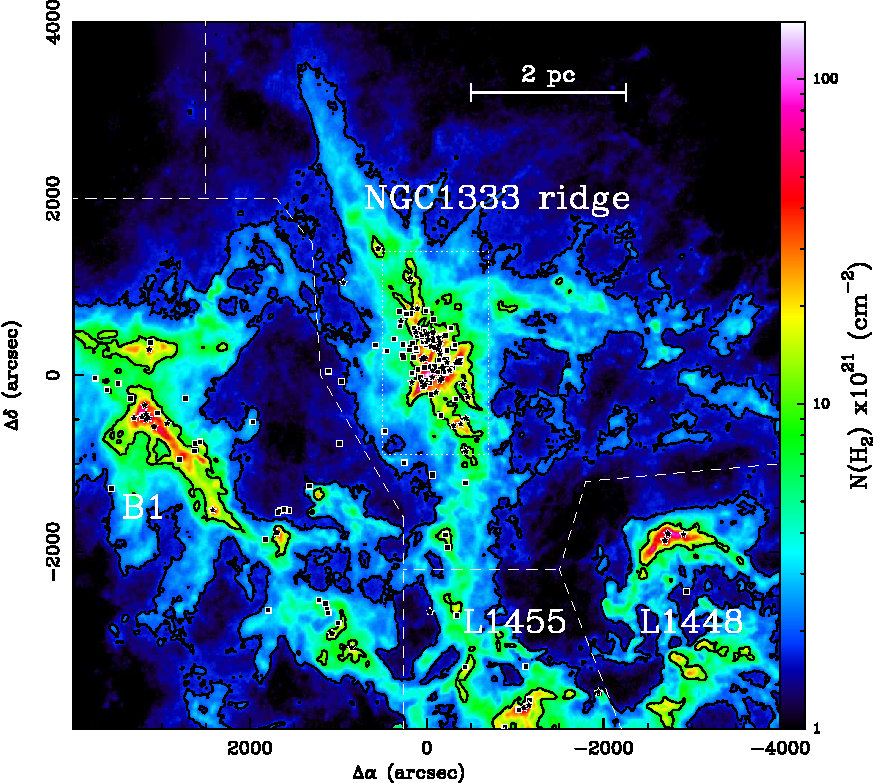
\includegraphics[width=\textwidth]{figures/NGC1333ridge.pdf}
		\caption[NGC~1333 ridge]{Column density map of the NGC~1333 ridge in Perseus, derived using Herschel-Planck maps \citep[taken from][]{hacar2017}. Offset coordinates are relative to the position RA(J2000)=$03^\mathrm{h}29^\mathrm{m}08\fs9$, Dec(J2000)=$31^\circ15\arcmin12\arcsec$. The squares and stars symbols represent the positions of the Class 0/I and Flat/ClassII/ClassIII objects, respectively \citep[for more information, see][]{hacar2017}.}
	\label{fig:NGC1333ridge}
	\end{center}
\end{figure}

% Star formation is traditionally divided into two parts: Low-mass stars form in a time short compared to the Kelvin-Helmholz time, tKH = Gm2∗ /RL, whereas high-mass stars form in a time ␃tKH (Kahn 1974). This distinction between low-mass and high- mass protostars is not fully satisfactory, however, because for a sufficiently high ac- cretion rate any protostar would be classified as low-mass. We somewhat arbitrarily divide low- and high-mass stars at a mass of 8 M␐ . Protostars that will form stars with masses significantly below this value have luminosities dominated by accretion, and they form from cores that have masses on the order of the thermal Jeans mass.  Protostars above this mass have luminosities that are dominated by nuclear burning unless the accretion rate is very high, and if they form from molecular cores, those cores are significantly above the thermal Jeans mass. \citep{mckee2007}

Completar: Star formation is relatively an inefficient process: on the cloud scale, only $\sim 5\%$ of the gas is converted into the stars; on the prestellar core scale, the star formation efficiency is about to $\sim$30-$\sim50\%$~\citep{offner2014, chevance2023}.

\subsection{The formation of a low-mass star}
% \subsection{Gravitational colapse of a dense core}
% \subsection{Evolution and classification of a forming solar-type star}
% \subsubsection{Prestelar phase}

As described in the previous section, low-mass stars form through the collapse of prestellar cores, gravitationally bound dense fragments of filaments within the molecular clouds. For a core to undergo gavitational collapse, self-gravity should overcome the oposing internal gas presure and, secondarily, the opposing forces due to magnetic field and turbulence. 

In an infinite sized cloud with no magnetic fields, turbulence nor rotation,\ \citet{jeans1902} showed that short-wavelength density perturbations propagates as sound waves that dissipate, but those perturbations that exceed the `Jeans length', $\lambda_J$, are gravity dominated and grow exponentially. For a isothermal uniform medium of density $\rho_0$ and temperature $T$, $\lambda_J=\pi^{1/2}c\left(G\rho_0\right)^{-1/2}$, where $c=\left(kT/m\right)^{1/2}$ is the sound speed, being $m$ the average particle mass. This imposes a minimum mass for the gravitational collapse; i.e., the `Jeans mass'; for a uniform sphere is 
%$M_J=8.53 c^3 G^{-3/2} \rho_0^{-1/2}$ \citep{larson1985, larson2003}.
$M_J=\pi/6\rho_0\lambda_J^3$.

The first numerical calculations of the gravitational collapse was performed by \citet{larson1969}, that considered a spherically symmetric cloud without taking into account magnetic fields, turbulence, and rotation. For the typical mean properties of cores (with masses of $\sim$1~$M_\odot$ and sizes of $\sim$0.1~pc), the collapse can be devided in four phases \citep{larson2003, estalella2008, schulz2012}:
\begin{itemize}
	\item Free-fall phase: Density increases isothermally (up to 10$^{-13}$~\gcmcu\ in the center) and matter falls in on a free-fall timescale. Ignoring presure gradients, the time needed for the collapse of a uniform sphere of gas is the free-fall time $t_\mathrm{ff}=(3\pi / (32G\rho))^{1/2}$, with a density distrubtion of the form $\rho\propto r^{-2}$.
	\item First core phase: Central density increases ($>10^{-13}$~\gcmcu) and some inner layers become optically thick, so the collapse is not isothermal and the contraction is adiabatic. The internal temperature and presure increases, so the core of a few au and $\sim$0.01~$M_\odot$ becomes stable; this is the First Hydrostatic Stellar Core, that continues to accrete mass through an accretion shock developed in its surface. 
	\item Opacity phase: Hydrogen molecules start to dissociate as internal temperature reaches $2000$~K. Since this process is highly endotermic, the internal pressure gradient is not able to enough to counter gravity, so this causes a second collapse. When density further increases to $10^{-2}$~\gcmcu as well as the ionization fraction of the hydrogen. Finally the collapse is permanently halted and a second hydrostatic core about $\sim$0.001~M$_\odot$ and radius $\sim$1~R$_\odot$ is formed: this is the `embryo' of the protostar.
	\item Accretion phase: The second core mass grows rapidly and, within a brief time, the mass of the first core falls into the second core. The main accretion phase starts and now the observations indicates the existance of a protostar. 
\end{itemize}

When rotation is taken into account \citep{bate1998}, these collapse phases are still valid, predicting the formation of a second hydrostatic core with similar properties. However, %when the initial rotation is included,
%because of the angular momentum conservation,
the remaining matter has a significant angular momentum, and an accretion disk will be formed around the protostar. Thus, accretion onto the star is disk mediated \citep{hartmann2016}. Accretion is intimately related to ejection phenomena, powerful collimated jets and winds along the rotation axis (see Fig. \ref{fig:accretion}). This ejections, that are thought to be driven by magnetocentrifugal forces from the disks, play an important role in removing angular momentum, allowing the star to reach its final mass \citep[e.g.][]{pudritz2019}. Observations indicates that these jets and winds are accretion-powered ejections, since mass loss rates strongly correlate with accretion luminosity \citep{cabrit1990, hartigan1995, cabrit2007, ellerbroek2013, natta2014, lee2020}.


% The classical collapse phases as described in the previous sections are valid with or without rotation and magnetic field support of the the collapsing core. In simple terms this means rotation and magnetic fields eventually cannot prevent the collapse once the core reaches critical initial conditions. The collapse will reach the first-core phase and its dynamical contraction will proceed as well. What will differ substantially is the matter flow onto the core as well as the dynamics of the infalling gas. \citep{schulz2012}

% In the presence of a finite outward pressure gradient, the collapse is somewhat decelerated from a free fall, but the time required for each radial mass shell to collapse to the centre is still approximately the free-fall time calculated from the average interior density of the shell. \citep{larson2003}

% Most calculations of the adiabatic phase of collapse have assumed spherical symmetry, but the fully three-dimensional calculation by Bate (1998) of the collapse of a slowly rotating prestellar cloud core predicts the formation of a second hydrostatic core that has properties similar to those found in the spherical case. When rotation is present, however, the remaining matter still has significant angular momentum and most of it will eventually settle into a disk around the central protostar; the later stages of evolution may then involve accretion from the disk (Yorke and Bodenheimer 1999). Disk accretion may play the same role in early stellar evolution as spherical accretion if the outward transfer of angular momentum in disks is efficient enough to yield a similar accretion rate (Mercer-Smith et al 1984). \citep{larson2003}

% Definition and properties molecular clouds \citep[e.g.,][]{mckee2007, hennebelle2012, dobbs2014}.
% GMCs \citep{chevance2023}.
% Hierarchical structure and hierarchical collapse \citep[e.g.,][]{vazquez-semadeni2019}.
% Filaments \citep{hacar2023, pineda2023}.
% Gravitational collapse of a dense cores \citep{larson2003}.
% % Dense, gravitationally bound molecular cores are the immediate precursors of stars. Generally speaking, ``dense cores'' can be used to refer to all overdense (relative to the background) structures at sub-pc scale, while ``clumps'' usually represent pc-scale complex structures that may further fragment into multiple cores.
% Low- and high-mass\citep{zinnecker2007, tan2014} star formation. Multiplicity: fragmentation of a turbulent core, disk fragmentation. Filament fragmentation, core fragmentation, disk fragmentation, and capture \citep{offner2023}.
% 


% \subsection{The star-disk-jet system}\label{sec:star-disk-jet}
% 
% The formation of a circumstellar disk is a natural outcome.
% Accretion onto the star is disk mediated.
% Accretion from the disk to the protostar \citep{hartmann2016}. 
% Role of ejections in removing angular momentum, allowing the star to reach its final mass \citep[e.g.][]{pudritz2019}.
% % From pudritz2019: The ability of torques exerted on disks by magnetized winds to efficiently extract and transport disk angular momentum was developed in early theoretical models and confirmed by a variety of numerical simulations. The recent high resolution Atacama Large Millimeter Array (ALMA) observations of disks and outflows now confirm several key aspects of these ideas, e.g., that jets rotate and originate from large regions of their underlying disks. New insights on accretion disk physics show that magneto-rotational instability (MRI) turbulence is strongly damped, leaving magnetized disk winds as the dominant mechanism for transporting disk angular momentum.
% Accretion-ejection link: accretion-powered winds.
% % No accretion disk implied no jet, although the converse was not necessarily true. It was also found that the strength of an outflow depended on the evolutionary status of the parent star: less evolved stars have more powerful outflows.
% Mass loss rates that strongly correlate with accretion luminosity \citep{cabrit1990, hartigan1995, cabrit2007, natta2014}.
% Launching mechanisms: Stellar winds, X-winds, disk winds\citep{pascucci2023, konigl2000, tabone2020}. \citep[Collimation and propagation of stellar jets, PPIV]{eisloffel2000}, \citep[Disk winds, jets, and outflows, PPV]{pudritz2007}. \citep{ferreira2006}
% Influence of jets on the physical properties of disks and, consequently, their role on their influence on the initial environmental properties related to planetary system formation \citep{ray2021}, which starts much earlier than previously thought \citep{harsono2018, segura-cox2020, alves2020}.
% 
% Accretion from the envelope to the disk.
% Streamers \citep{alves2019, pineda2020, valdivia-mena2022, pineda2023, flores2023}. 
% 
% Figure of a scheme of the star-disk-jet system. \citet{lee2020}?

\begin{figure}[h!] 
	\begin{center}
		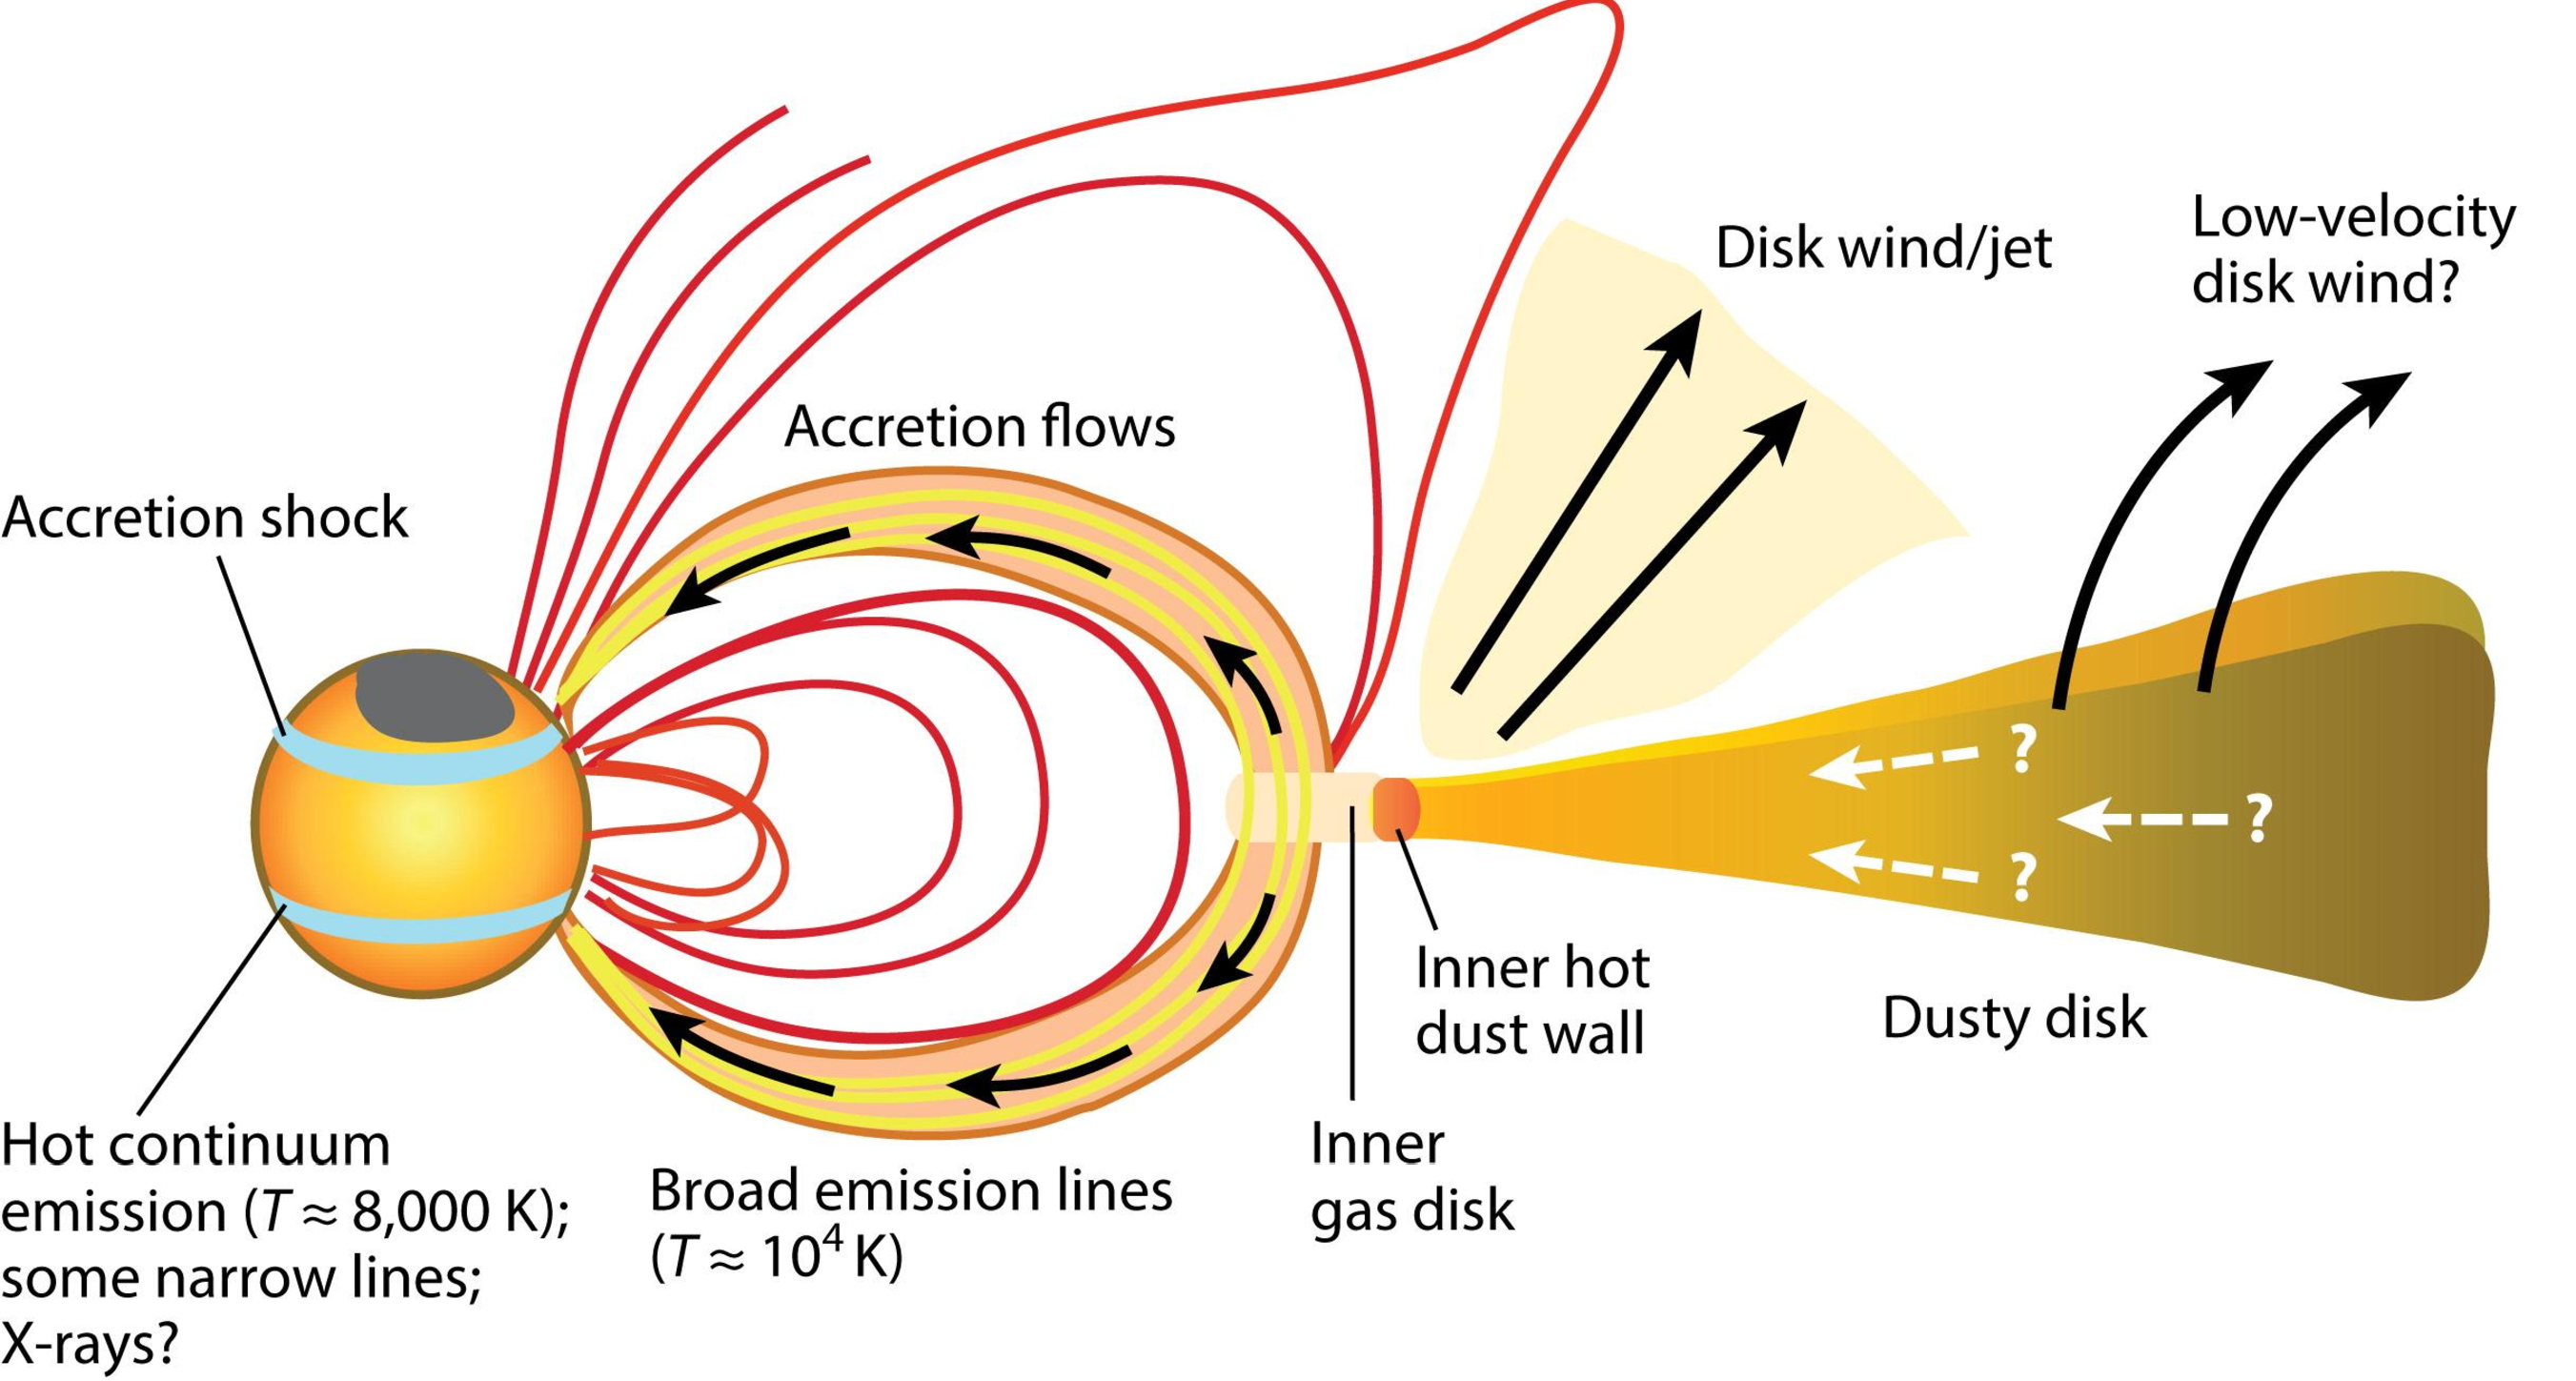
\includegraphics[width=\textwidth]{figures/hartmann2016.png}
		\caption[Outflow and jet scheme]{Taken from \citet{hartmann2016}}
	        \label{fig:accretion}
	\end{center}
\end{figure}

\subsection{Classification and evolution of Young Stellar Objects}
% \subsection{Classification of Young Stellar Objects}
The evolution of an isolated low-mass Young Stellar Object (YSO) has been traditionally characterized from the shape of the spectral energy distribution (SED), using the IR spectral index between 2.2 and 100~$\mu$m \citep{andre2000, dunham2014b}:

\begin{equation}
	\alpha_{\rm IR} = \frac{d\log\lambda F_\lambda}{d \log\lambda}
\end{equation}

\begin{figure}[h!] 
	\begin{center}
		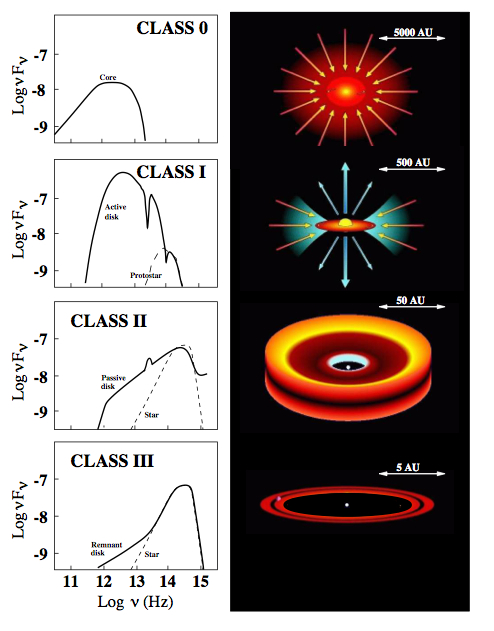
\includegraphics[height=0.8\textheight]{figures/YSOclassification.jpg}
		\caption[YSO classification]{Scheme of the classification and evolutionary stages of a isolated YSO.}
	        \label{fig:YSOclassification}
	\end{center}
\end{figure}

\begin{itemize}
	\item Class 0:  Protostars in this phase are highly embeded in a cold ($T=10$-$30$~K) and dusty envelope \citep{andre2000}. Consequently, this type of objects are extremely faint in the optical and near-IR, and are submillimeter sources. The SED resembles to a cold black body, characteristic of the natal cold envelope, which still contains most of the final mass. An accretion disk is already formed, with a mass of $\sim10\%$ of the mass of the envelope. Accretion processes are high, which is accompanied by powerfull outflow phenomena. These are the youngest YSOs, with ages $\lesssim 10^4$ yr.
	\item Class I: This protostars are still embeded in the envelope, but most of the mass is contained in the circumstellar disk and the protostar. Thus, this objects are detected in the near infrared, but are not optically visible, and they are characterized by $0<\alpha_\mathrm{IR}\le 3$. Although still associated with outflow phenomena, since accretion is less important, they are less powerful than Class 0 objects. The age of these objects ranges between $\sim 10^4$-$10^5$.
	\item Class II: These YSO are no longer in the protostellar phase, and are regarded as pre-main-sequence stars. The enveloped is almost cleared out, and are characterized by $-2<\alpha_\mathrm{IR}\le 0$. Consequently, they can be detected in the optical and in the infrarred; they are classical T Tauri stars. Disks can clearly be observed in the submillimeter weavelengths, which presents rings and gaps; the signatures of forming planets. Their ages ranges between $\sim10^5$-$10^6$~yr.
	\item Class III:. At these phases, the disk is almost cleared out, which can host recently formed planets, and there is almost no further accretion to the protostar. Thus, accretion and ejection processes are negligible. The SED resembles to one of a black body at a high temperature, characteristic of the photosphere of the star. The IR spectral index is in the range of $-3<\alpha_\mathrm{IR}\le -2$. Their ages ranges between $\sim10^6$-$10^7$~yr.
\end{itemize}

% Evolution of an isolated low-mass YSO. 
% \citep[Review]{dunham2014b}
% \citep[for class 0]{andre1993}
% \citep[PPIV review]{andre2000}


% Trends to metion:
% Mass accretion and mass-loss is decreases from Class 0 to Class II \citep{ellerbroek2013} (show figure2 from \citet{lee2020}). In Class III, accretion and ejection processes are negligible.
% The velocity of the jets for Class 0 is smaller than that of Class I and II jets.
% The mass-loss rate of Class 0 is larger than that in class I and II. 
% %As The YSOs evolve, the velocity of their primary winds or jets tends to increase, transitioning from predominantly molecular to mostly atomic and partially ionized plasma. Tswept-up shells traced by CO become less prominent as they widen, sweep up more mass, and decelerate. As outflows break out of their parent cloud cores, their internal shocks are best traced by chains of HH objects.  Outflow cavities are wider with age \citep{offner2011}
% Class 0 disks are smaller than Class I and II \citep{maury2019}.
% % Class 0 \citep{andre1993}: ``The mass ejection of VLA 1623 appears to be extremely efficient and implies that a global MHD approach to infall and outflow may be required to explain the youngest embedded sources. It is suggested that VLA 1623 and a few other low-luminosity YSOs make up an entirely new class of YSOs. ''
% 

%\section{Observations of jets and outflows}
% \section{Protostellar jets and outflows}
% \section{Ejections from protostars}
% \section{Outflows from protostars} 
% \section{Outflows from young stellar objects}

% \section{Jets and outflows from young stellar objects}

%\subsection{Multiple star formation}
\subsection{Multiplicity in star formation}

Multiplicity: fragmentation of a turbulent core, disk fragmentation. Filament fragmentation, core fragmentation, disk fragmentation, and capture \citep{offner2023}.

\subsection{Signatures of variable accretion in Young Stellar Objects}

\citep{fischer2023}, \citep{audard2014}




\section{Outflow manifestations of Young Stellar Objects}

% ray2021: Jets are ubiquitous in the Universe and are seen from a large number of astrophysical objects, including activ galactic nuclei, gamma ray bursters, micro-quasars, proto-planetary nebulae, young stars and even brown dwarfs. In eery case they seem to be accompanied by an accretion disk and, while the detailed physics may change, it has been suggested that the same basic mechanism is responsible for generating the jet.aied by an accretion disk and, while the detailed physics may change, it has been suggested that the same basic mechanism is responsible for generating the jet. Although we do not understand what that mechanism is, or even if it is universal, it is thought to involve the centrifugal ejection of matter from the disk along magnetic field lines. For a number of reasons, in particular their proximity and the abundant range of diagnostics to determine their characteristics, jets from young stars and their associated outflows may offer us the best opportunity to discover how jets are generated and the nature of the link between outflows and their accretion disks.

Outflows are an ubiquitous ingredient of the star formation process. Moreover, they are not a mere by-product of the protostar evolution, but they play an important role in the assembly of stars, can alter the properties of the protoplanetary disks and, consequently, they might be able to have an impact also on the planet formation process \cite{frank2014}. Also, comment the role at molecular cloud scale.
% Star formation process involve accretion-powered ejections

% SEA proceedings: Outflows from young stellar objects usually present two different components. A highly-collimated and partially ionized component (the jet), which is traveling at extremely high velocities ($\sim$100~km/s), and a fairly collimated (and usually bipolar) component (the molecular outflow) with velocities of the order of 10 km/s. Jets are originated from the proximity of the star (likely from its accretion disk) and frequently observed at optical, infrared and radio wavelengths \cite{bally2016, anglada2018, ray2021}. Jets are thought to be powerful enough to entrain ambient gas and produce the usually more massive molecular outflows ubiquitously observed in low-excitation transitions of CO and other molecular species at mm wavelengths \cite{rodriguez1982, lada1985, bachiller1996, lee2020}.

% They are not a mere byproduct.
% Moreover, they are not a mere by-product of the protostar evolution, but they play an important role in the assembly of stars, can alter the properties of the protoplanetary disks and, consequently, they might be able to have an impact also on the planet formation process. Also, comment the role at molecular cloud scale: effects on the star formation efficiency.

% \subsection{A historical review}
\subsection{A brief historical review}
% The fact that is accompanied  is accompanied by These powerful ejections were unanticipated by theorists \citep{stahler2004}. It was not until the 80s when there was enough observational evidences that star formation was accompanied by powerful ejections.
% Bally2007: Although no theory anticipated jets and outflows, it is now clear that they are a fundamental aspect of star formation.
It was not until about 1980 that there was sufficient observational evidence to show 
% to show
that star formation was accompanied by powerful ejections, which were unanticipated by theorists. Thus, the star formation paradigm changed from a infall only scenario into one in which outflow phenomena was a fundamental aspect. % \citep{stahler2004}.
% into one in which outflow activity was also associated with all stages of the early stellar evolution.

% The observational evidences that led to this conclusion
The discovery of outflows from YSOs
% that led to the conclusion that outflows was an ubiquitous aspect in star formation
% that forming stars present outflows
can be traced back to the first observations the Herbig-Haro (HH) objects, which were independently discovered by George Herbig \citep{herbig1951, herbig1952} and Guillermo Haro \citep{haro1952}.
%; for some nice reviews on the discovery and the properties of HH objects, see \citet{schwartz1983}, \citet{reipurth1997}, and \citet{reipurth2001}.
HH objects are nebulae with a size of 20-30\arcsec, often found in pairs or strings, detected in the optical, dominated by hydrogen Balmer emission lines and other lines as [O II], [S II], or [FeII] \citep{schwartz1983, reipurth1997, reipurth2001}. Although it was clear that HH objects were related with some aspect of star formation, they were initially interpreted to be nebulae where the formation of a star was taking place \citep{herbig1969}.
%where stars were forming~ \citep{herbig1969}.
%It was not until 25 years later \citep{schwartz1983}
The shock nature of the HH objects was revealed by \citet{schwartz1975} who, based on the similarity between the HH spectra and the ones of the knots in supernova remnants, suggested that HH objects resulted from the interaction of YSO ejections with the ambient gas. Interestingly, with the development of infrared astronomy in the 1970s, it became clear that the driving sources of the ejections were not located in the nebulae, but the sources appeared at some distance.
%Strong observational evidences \citet{schwartz1975} suggested that HH objects were associated to shocks the interaction of stellar ejection with ambient gas, based on the base of the similarity between the HH spectra and the ones of knots in supernova remnants.
% This interpretation was completely accepted
% This interpretation was confirmed
% Further evidences that supported this interpretation 
% This interpretation was further supported 
The interpretation that HH objects resulted from powerful ejections from the protostar was further supported
when large proper motion (corresponding to tangencial velocities of $>100$~\kms) of HH objects were measured \citep{cudworth1979,herbig1981, jones1983}.
%It was accepted that they are the results of the interaction of the high velocity stellar winds with the ambient molecular gas. 
% The detection of Herbig–Haro (HH) objects [453–456] happened soon after the discovery T Tauri stars. Quickly it was realized that the nebula found around the star T Tau and HH objects have remarkable similarities. \citep{schulz2012}
% They were thought to be protostars themselves.
% protostellar condensations or reflection nebulae, the actual ``cradles'' of stars. 

% Interesting, there were observational evidences of winds from protostar from 1964 (Kuhi et al. 1964), from ferreira2007: Prior to the discovery of HH jets, it was already evident that YSOs had outflows. Winds from young stars, for example had been discovered many years before (Kuhi et al. 1964) but perhaps more pertinently observations of star forming regions using molecular lines (e.g. CO rotational transitions) at mm wave- lengths revealed giant redshifted and blueshifted lobes straddling opposite sides of protostars.

\noindent
% Discovery Herbig-Haro objects (HH were independently discovered by George Herbig
% %\citep{herbig1950} por alguna razón este artículo no se cita, si no el de 1951 (ver schwartz1983, ray2021, shang2023)
% \citep{herbig1951, herbig1952} and Guillermo Haro \citep{haro1952})
% % schwartz1983: in the course of Halpha-emission star surveys of a dark-cloud region immediately south of the Orion Nebula. The prototype objects HH1, 2, and 3, located near NGC 1999, each exhiit structure with tightly grouped knot-like condensations. The spectra of HH objects are usually dominated by hydrogen Balmer emissionlines and low-excitation emission lines of [OI], [SII], [NI], [FII], with moderate strength [O II] and [N II] lines, and relatively weak [O III] emission. Their locations in or near dark clouds in regions of star formation led to early speculation that the objects are associated with processes of star formation. Indeed, their properties and apparent lack of coincidence with visible young stars (e.g. T Tauri stars) led to the suggestion that HH objects are themselves the sites of prestellar activity (cannot find the references) [\ldots] but the truth is that the HH objects are the by-produts of star formation rather than incipient stars.
% % Ray2021: In the 1950s, Herbig (1951) and Haro (1952) discovered the nebulous patches in Orion that now bear their name. At first these were thought to be actual ‘‘cradles’’ of stellar birth and it was not until the 1960s that Schwartz (1977) realized that Herbig–Haro (HH) objects may be part of an outflow from a young star. This he thought likely because their spectra bore certain similarities to the shock ejecta from supernova remnants.
% % According to Schwartz1983 the discovery of the HH is also acknowledge through a Private communication from Haro, G (1950) of May 31 to Drs. H. Shapely and R. Minkowsky. This comunication is mentioned in the \citet{haro1952}
% \citep[Review on HH]{schwartz1983},
% \citep[Review on HH]{reipurth2001},
% \citep[very nice historical review]{reipurth1997}.
% HH were initially thought to be protostellar condensations or reflection nebulae.
% \citet{osterbrock1958} suggested that the excitation of the HH objects might result from an energetic outflow of material from a young star.
% %The similarity of the spectra between the HH nebule and the quasistationary knots in supernova remnants led \citet{schwartz1975} to suggest that the classical HH objcts are the result of the interaction of a supersonic stellar mass outflow with ambient gas, creating radiative shocks.
% \citet{schwartz1975} suggested that the classical HH objcts are the result of the interaction of a supersonic stellar mass outflow with ambient gas, creating radiative shocks.
% % They were initially thought to be protostellar condensations or reflection nebulae (citations?). According to \citep{schwartz1983}, \citet{osterbrock1958} was the first to suggest that the excitation of the HH objects might result from an energetic outflow of material from a young star. It was accepted later that they are the result of the interaction of high-velocity stellar winds with the ambient molecular gas. The similarity of the spectra between the HH nebule and the quasistationary knots in supernova remnants led \citet{schwartz1975} to suggest that the classical HH objcts are the result of the interaction of a supersonic stellar mass outflow with ambient gas, creating radiative shocks.
% Large proper motion of HH by \citet{herbig1981} \citep{jones1983}. It was accepted that they are the results of the interaction of the high velocity stellar winds with the ambient molecular gas.

% The near-IR (Strom, Grasdalen, and Strom 1974; Cohen and Schwartz 1979) and radio (Rodriguez et al.  1978, 1980; Haschick et al. 1980) observations have revealed that often there are heavily obscured proto- stellar or pre-main-sequence objects of medium to high luminosity (10-104 L0) in the proximity (0.1- 1 pc) of the HH objects, but clearly not coincident with them.

The first molecular outflow associated to a protostar was dicscovered in CO in the molecular cloud L1551 \citep{snell1980}
% in radio
with the Millimeter Wave Observatory (MWO). The emission was bipolar, poorly collimated, with a size of 0.5~pc and velocities of $\sim 15$\kms, with the presence of two HH objects in the blue lobe. \citet{snell1980} proposed that the bipolar molecular outflow was material from the stratified molecular environment that was being swept-up by an initially isotropic wind.

% \citet{dopita1982} reported evidences that the HH 46/47 objects form a bipolar ejection emanating from a young star.

% The fact that HH objects was related with a bipolar outflow was insightful

% jetsfromyoungstars2007: Some 60 of these “molecular outflows” had been discovered by the mid 80’s alone [36]. In all cases they appeared to be poorly collimated with typical velocities of tens of km s−1 and sizes between 0.1 – 1 pc (e.g.  [6])

%!!
% \citet{dopita1982} reported evidences that the HH 46/47 objects form a bipolar ejection emanating from a young star.
%!!

In the early 1980, the widespread use of CCD in astronomy allowed much deeper images than photographic plates. From observations with the 2.2~m telescope of the Calar Alto Observator, \citet{mundt1983} reported four optical highly-collimated emission (jets), emanating from young stellar objects, with observed velocities >100~\kms, some times connected to HH objects. Thus, it was interpreted that the HH knots were parts of these 
%highly collimated emission (or jets),
jets where the interaction with the surrounding medium was taking place.

%Thus, it was interpreted that the HH knots were working surfaces of the jets, meaning that the knot is due to the thermalization of the kinetic energy in the jet as it hits the surrounding medium.


% Mundt1983: Our Ha-CCD frame (iexp = 0.4 hr) shows a bright HH knot 8" SW of DG Tau (P.A. = 228° ± 2°) ap- parently connected with the star by a “fight bridge,” or jet (Fig. 5, Plate L10).


% and the first jets were detected. 
% 
% In the early 1980, the widespread use of CCD in astronomy allowed much deeper images than photographic plates, and the first jets were detected. 
% 
% From observations with the 2.2~m telescope of the Calar Alto Observator, \citet{mundt1983} reported four optical jets emanating from young stellar objects. Thus, it was interpreted that the HH knots were working surfaces of the jets, meaning that the knot is due to the thermalization of the kinetic energy in the jet as it hits the surrounding medium.

% All dots were connected when after the development of the CCD, which allowed much deeper images than photographic plates, the first jets, which connected the forming star with HH-objects, where detected. From observations with the 2.2 m telescope of the Calar Alto Observator, \citet{mundt1983} reported four optical jets emanating from young stellar objects.

% First molecular outflow associated to a protostar observation in CO in the molecular cloud L1551 \citep{snell1980}.
% % Bipolar 15~\kms\ The emission was bipolar, and one of the lobes is associated with a HH. Thus, Snell propose that the molecular flow was molecular material from the envelope that was being entrained by an internal wind. % overview with empahsis on the radio:\citep{canto1981}
% % \citet{dopita1982} realized that the HH 46/47 objects form a bipolar jet emanating from a newborn star.
% \citet{dopita1982} reported evidences that the HH 46/47 objects form a bipolar ejection emanating from a young star.
% \noindent
% From observations with the 2.2 m telescope of the Calar Alto Observator, \citet{mundt1983} reported four optical jets emanating from young stellar objects.
% % DG Tau, DG Tau B, HH 30, HL Tau
% % \citep{mundt1983} published their highly influential paper about jets from young stars, in which they presented the discovery of four HH jets.
% % First optical jet with he 2.2 m telescope of the Calar Alto Observator \citep{mundt1983}.
% % 100 km/s.
% % but see also Dopita 1982 MA, Schwartz RD, Evans I. 1982b, Ap.J. 263:L73-77. According to reipurth2001, ``The recognition that some HH objects take the form of highly collimated “jets” (e.g., Dopita et al. 1982b, Mundt & Fried 1983) was central to the development of our current concept of HH objects as the visible manifestations of collimated outflows from young stars.''
% 
% % Current observations of jets and molecular outflows.
% %Traditionally
% % Typically, ejections from protostars have been observed as jets, 
% % highly-collimated gas traveling at velocities of the order of 100-1000~\kms
% % ; and molecular outflows, less collimated than jets, with velocities of \sim10~\kms.
% 
% % Typically, ejections from protostars have been observed as jets and molecular outflows.
% % % Traditionally, ejections from protostars have been classified into jets and molecular outflows.
% % % ; and molecular outflows, less collimated than jets, with velocities of \sim10~\kms.
% % Jets are high collimated structures of gas traveling at velocities of the order of 100-1000~\kms.
% % %Jets are thought to be launched through magnetohydrodynamic (MHD) mechanisms in the rotating star-disk system. They are traced in the optical, infrared, and in the cm. 
% % Molecular outflows are less collimated than jets, with velocities of \sim10~\kms.

Typically, ejections from protostars have been observed as jets and molecular outflows:
% Traditionally, ejections from protostars have been classified into jets and molecular outflows.
% ; and molecular outflows, less collimated than jets, with velocities of \sim10~\kms.

\begin{itemize}
	\item Jets are high collimated structures of gas traveling at velocities of the order of 100-1000~\kms.
% Jets
are thought to be launched through magnetohydrodynamic (MHD) mechanisms in the rotating star-disk system. Usually traced in the optical, infrared. Also in the cm, radio jets. The youngest sources have also a molecular component, traced in CO and other molecules in the mm. Usually called ``molecular jets''. Molecular bullets. %(as SiO, and SO).

 \item Molecular outflows are less collimated than jets, with velocities of $\sim$10~\kms. Ubiquitously observed in CO and other molecules in the mm. Bipolar. The classical picture is that they consist of gas entrained by a jet or a wide-angle wind. Nevertheless, ALMA is detecting small-scale molecular outflows ($\leq$2000$\sim$au). Rotation. They are thought to be MHD-winds, so they are sometimes called ``molecular winds'', to be distinguished from the classical bipolar molecluar outflows of swept-up ambient gas at larger scales.

 \end{itemize}
\begin{figure}[t]
	\begin{center}
		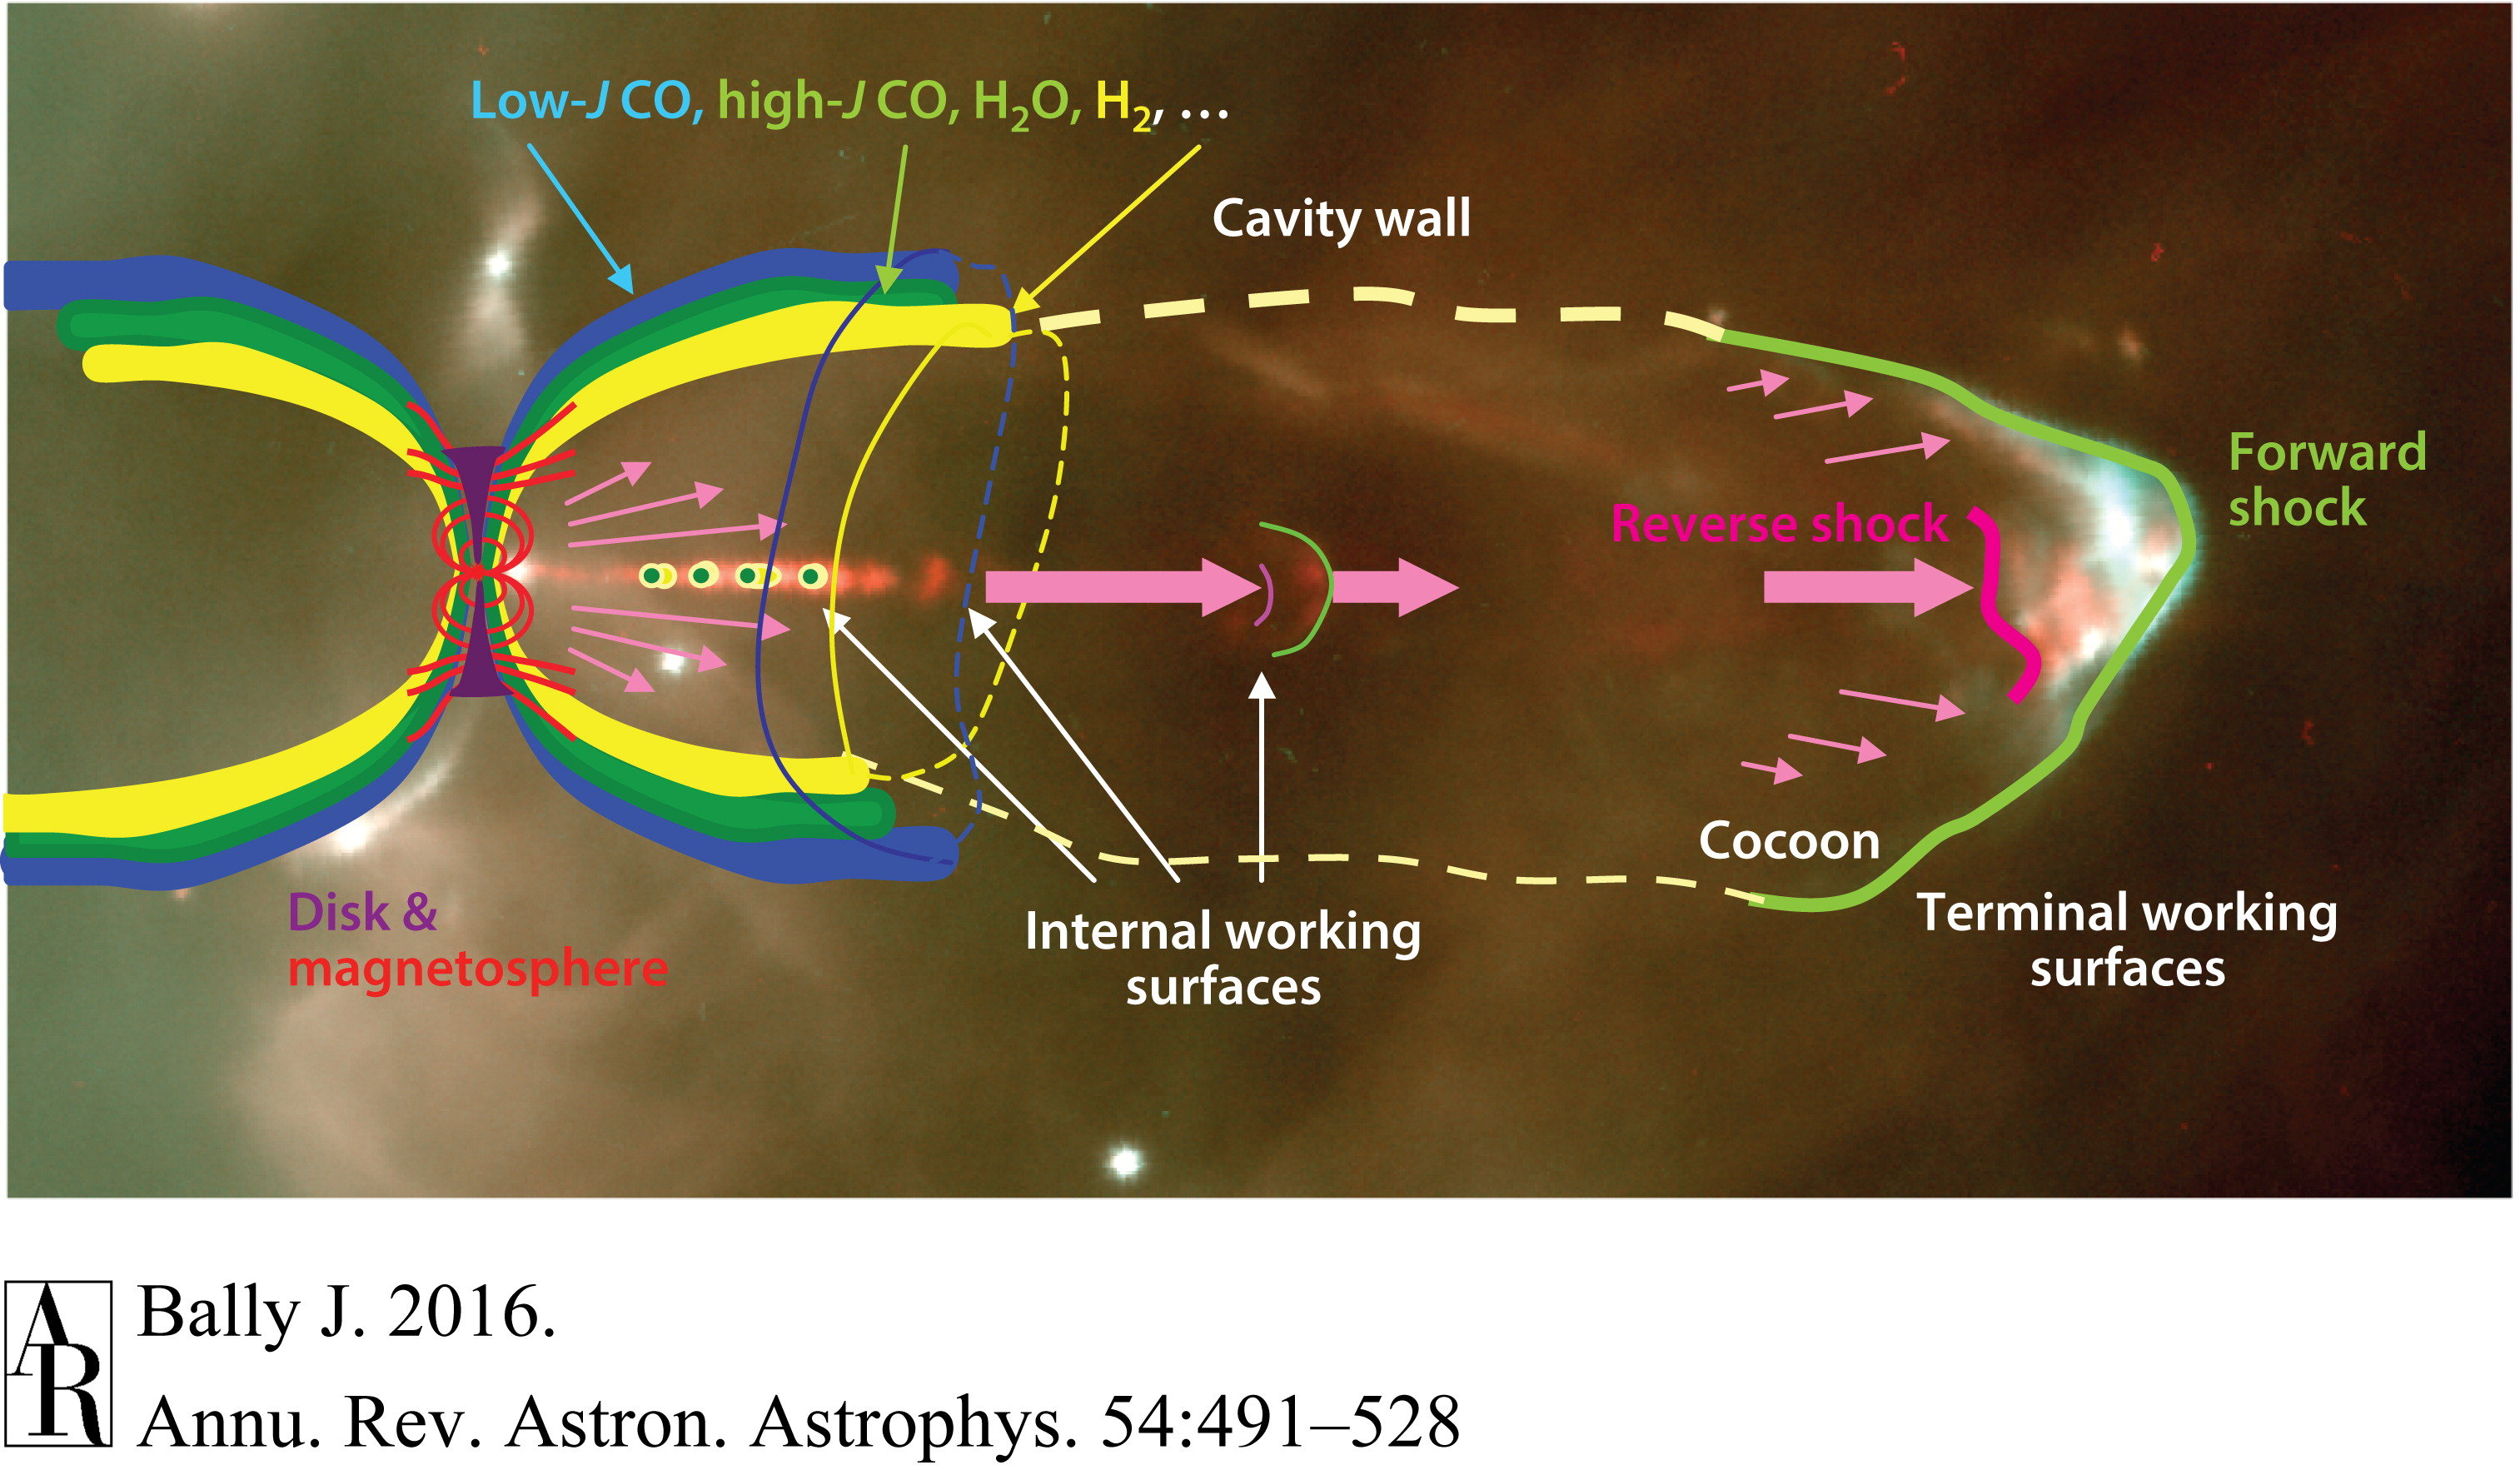
\includegraphics[width=\textwidth]{figures/bally2016_outflow.png}
		\caption[Outflow and jet scheme]{Taken from \citet{bally2016}}
	\end{center}
\end{figure}


% Adopted nomenclature: 
% Outflow: General term for flow of gas associated to a protostar. It is usually used for the large scale molecular outflow, which is the edge of the cavity of low-velocity gas entrained by a jet or wind. But it can be the driving agent (it can be originated in the protostar or its vecinity), so jets and winds are also outflows.
% Jet: Collimated outflow originated from the protostar or its vecinity. Can drive large scale (and lower velocity) molecular outflow. Jets can be molecular also.
% Wind: Outflows originated from the protostar or its vecinity, less colimated than jets. Wide-angle winds can drive large scale molecular outflows. Winds can be molecular also.
% \subsection{Molecular outflows}

% \subsection{Large-scale molecular outflows}
\subsection{Molecular outflows}
% \section{Large-scale bipolar molecular outflow}
% \section{Classical molecular outflow}
% \subsection{Large-scale molecular outflows}
% Large-scale molecular outflows
% \subsection{Interaction with the envionment}

Properties \citep[e.g.][]{lada1985, cabrit1997, bally2007, arce2007, bally2016}. Scales. Tracers. Velocities. Hubble-law \citep{lada1996}. Dynamical times? Evolution with source spectral class. Mass law with velocity as $dM/dv\propto v^{-\gamma}$. Large masses: the material can not originate from the YSO, and must consist primarily of ambient material swep-up by a momentum flux emanating from the YSO. Also, they can not be driven by radiation pressure since the momentum in outflows is several orders of magnitude greater than that which can be supplied by radiation pressure from YSO \citep{bally1983}. Large-scale molecular outflows can be driven by jets or wide-angle winds \citep{lee2000, lee2001, arce2007}.
% Due to the tremendous mass of large scale molecular outflow, the material can not originate from the YSO, and must consist primarily of ambient material swept up by a momentum flux emanating from the YSO. They can not be driven by radiation pressure since the momentum in outflows is several orders of magnitude greater than that which can be supplied by radiation pressure from YSO \citep{bally1983}.Thus, molecular outflows must be ambient material swept up by mass ejecting from the YSO. The issue is to determine whether molecular outflows are driven by purely collimated jets or by wide-angle radial winds with a high density ``jet-like'' core. \citep{lee2000} \citep{lee2001}

% \citep[Models for bipolar molecular outflows]{cabrit1997}
% \citep[PPV Review]{bally2007b}
% \citep[PPV Review]{arce2007}
% \citep[PPVI Review]{frank2014}

% \subsubsection{Jet-driven models}
% Jet interaction with the environment:  
% Jet interaction with the environment. Large-scale molecular outflow. Due to the tremendous mass of large scale molecular outflow, the material can not originate from the YSO, and must consist primarily of ambient material swept up by a momentum flux emanating from the YSO. They can not be driven by radiation pressure since the momentum in outflows is several orders of magnitude greater than that which can be supplied by radiation pressure from YSO \citep{bally1983}. Thus, molecular outflows must be ambient material swept up by mass ejecting from the YSO. The issue is to determine whether molecular outflows are driven by purely collimated jets or by wide-angle radial winds with a high density ``jet-like'' core. \citep{lee2000} \citep{lee2001}

Jet-driven: Description of the jet-driven model. (semi)-analytic models \citep{raga1993, masson1993, ostriker2001}, simulations \citep{chernin1994, smith1997, suttner1997, downes1999, downes2007, rabenanahary2022}. The collimated jet propagates and interacts with the environment, and a two shock structure (called ``working surface'') is created: one shock inside the jet, the ``jet shock'' (or Mach disk), formed as the fast jet material impacts the slower previously shocked material; and the other shock in the environment, the ``bow shock'', formed as the shocked material impacts the quiscent ambient material \citep{hollenbach1997, raga2021}.
Due to the high thermal pressure between the shocks, the material in the jet beam is expelled sideways through the working surface, interacts with the ambient and a swept-up shell is formed surrounding the jet. 

%interacts with the unperturbed ambient gas, where a bow-shaped thin layer of turbulent mixed (ambient+jet) material is formed surrounding the jet \citep{raga2021}. The large scale molecular outflow is the swept-up shell.

% The jet shock slows down the jet material, and the bow shock accelerates the ambient gas. The thermal pressure of the shocked material is expelled sideways and interacts with the unperturbed ambient gas, where a bow-shaped thin layer of turbulent mixed (ambient+jet) material is formed surrounding the jet \citep{raga2021}. The large scale molecular outflow is the swept-up shell.

% The thermal pressure of the shocked material expands expands sideways out of the jet beam throguh the working surface into the ambient material. As the shocked material flows sideways into the ambient material, it forms a bow shock surface sweeping accros the ambient material, producing a thin swept-up shell of shocked material surrounding the high-temperature but low-pressure cocoon which in turn surrounds the jet. 
%The working surface is the surface surrounding the shocked material between the jet and bow shock . The total momentum delivered by the jets
% Let us consider the propagation of the head of a jet into an environment which is stationary with respect to the outflow source (this is called the “starting jet” problem in the non-astrophysical literature). For the case of a hypersonic  jet, the head of the jet has a two-shock structure (called a “working surface”), with a “jet shock” (or Mach disk) which slows down the jet material and a “bow shock” which accelerates the environmental gas. This shock structure is schematically shown in Figure 14.1.  If the jet is instantaneously “turned on”, the two shocks in the working surface will initially be spatially coincident, and they separate until an approximately steady configuration is formed (in which the material entering the working surface from the jet and from the environment is balanced by a sideways ejection).  In this steady configuration, the bow shock and the jet shock travel away from the outflow source with the same velocity vws.
%taking into account both the density corrections implied by their partial ionization state and the long lifetimes indicated by the detection of pc-scale outflows,
The total momentum delivered by jets appears to be consistent with that measured in the associated CO outflows \citep{hartigan1994, eisloffel1997}
% \subsubsection{Jet-driven models}
% Jet-driven bow shock model
% In addition to the leading working surface at the head of the jet, time variability in the jet's velocity can produce a series of internal working surfaces along the jet \citep{raga1990}.
% \citep{raga1990} In addition to the leading working surface at the head of the jet, time variability in the jet's velocity can produce a series of internal working surfaces along the jet.
% See also: 
% \citep{masson1990, masson1993, ragacabrit1993}
% \citep{masson1993}
% \citep{ragacabrit1993}

% \subsubsection{Wind-driven models}

Wide-angle wind-driven:
The outflow is produced by a radially expanding wide-angle wind that is sweeping up the surrounding ambient material \citep{shu1991, shu2000}. Extended by \citep{li1996, matzner1999}. In this scenario, outflows are a purely momentum-driven phenomenon. The angular distribution of the ambient density and wind density, produce a shell geometry that have been compared with molecular outflows. In the ``unified model'' proposed by \citet{shang2006}, the jet is the central core of a wide-angle wind whose density decreases away from the axis (see also \citep{shang2020, shang2023}).
% See more on leephdthesis2000

% The wind can be stratified in density if it emerges from an extended disk (e.g. Ostriker 1997) or by the action of latitudinal magnetic stresses in a rotating protostellar x-wind (shu et al. 1995). 

% \citep[First paper of the self-similar, radially expanding shell driven by a wide-angle stellar wind]{shu1991}


% \subsection{Origin of jets}
% \subsection{Origin of jets and entrainment}
% \subsection{Origin of jets and winds}
% \subsection{Scenarios for jets from young stellar objects}
% \subsection{Jet launching mechanism} 
% \subsection{Driving mechanisms}
% \subsection{Jet driving mechanisms}
% \subsection{Small-scale molecular outflow: molecular winds}
% \subsection{Molecular winds}
% \subsection{Small-scale molecular outflow: rotating molecular winds}
% \subsection{High resolution observations towards the base of molecular otuflows}
% \subsubsection{Small-scale rotating molecular winds}\label{sec:molecularwinds}
%\subsection{Molecular winds}\label{sec:molecularwinds}
\paragraph*{Molecular winds}%\label{sec:molecularwinds}


New result from submm interferometers, particularly ALMA. Properties. The rotating flow is confined inside of the main swept-up outflow cavity walls.
\citep[Review]{pascucci2023}:
% Pascucci2023: A kewy new result provided by submm interferometers is the discovery of small-scale ($\leq$2000~au) molecular flows around a growing number of low-mass Class I/0 sources that rotate in the same sense as the disk and ar rooted within the disk at radii $\leq10-100$~au. This geometry hints at materila directly ejected from the disk surface. In addition, in HH 212, the rotating flow is confined inside of the main swept-up outflow cavity walls delineated in CO and CS \citep{tabone2017}., and inside the dense flattened rotating infalling envelope traced by HCO$^+$ \citep{lee2021}. Therefore, in the following, we will refer to these small-scale rotating flows as molecular winds to distinguish them from the classical bipolar molecular flows of swept-up ambient gas observed over much larger (parsec) scales around embedded sources \citep{arce2007, frank2014}. 
% Devalon: Thanks to the advances in the mm radio interferometry (in particular ALMA), we have obtained with unprecedented sensitivity and spetral resolution observations towards the base of the outflows in the last decade. The high angular resolution makes possible ot observe the base of the molecular flows and detectsmall-scale velocity gradients.
% See louvet phd thesis for a nice table of the properties
Scales ($\leq$2000~au).
Morphology: conical or parabolic shapes, semi-opening angles 10-40$^\circ$.
%and an inner low-brightness ``cavity'' surrounding the jet beam.
Tracers.
Velocities.
Dynamical times?
Masses.
% Hubble law?
Rotation, why is important and quantify.
They are thought to trace matter directly ejected from the disk by thermal or magnetic processes.
Consistent with launching radii XX-XX au.
Examples: 
Class 0: HH212 \citep{tabone2017, lee2018_HH212, tabone2020, lee2021},
HH211 \citep{lee2018_HH211},
NGC1333-IRAS4C \citep{zhang2018}.
Class I: 
CB26 \citep{launhardt2009, launhardt2023, lopez-vazquez2023},
TMC1A \citep{bjerkeli2016},
DGTauB \citep{zapata2015, devalon2020, garufi2020, devalon2022};
Class II:
HH30 \citep{louvet2018},
HD~163296 \citep{booth2021}.

And also high-mass YSOs: Orion Source I \citep{hirota2017, lopez-vazquez2020}.
% Lopez-vazquez have worked on HH30 rotating outflow. Is it not published yet?

Fig 2 from Pascucci 2023?
\begin{figure}[h]
	\begin{center}
		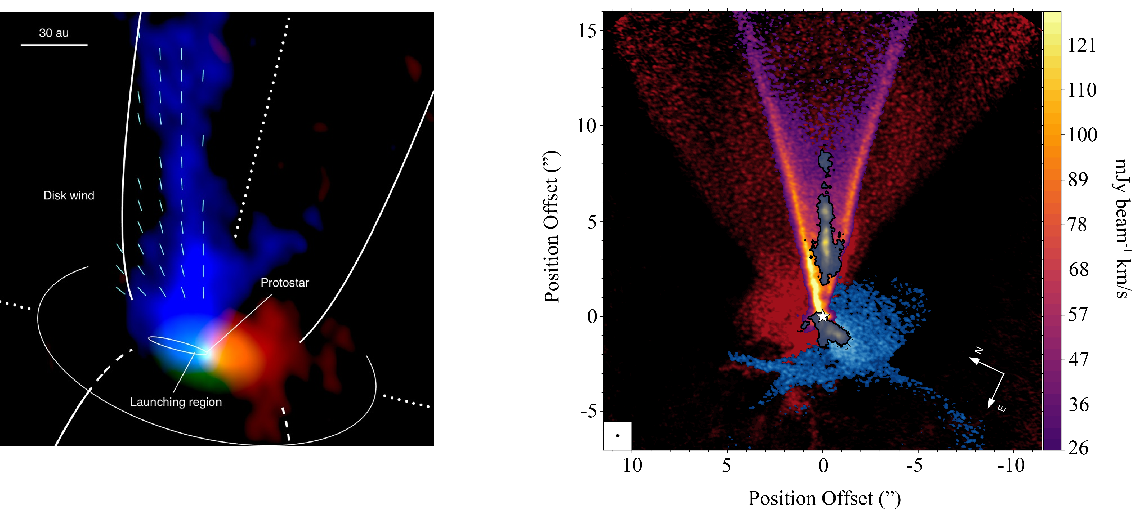
\includegraphics[width=\textwidth]{figures/molecularwinds.pdf}
		\caption[Molecular winds]{Left: \citet{bjerkeli2016}. Right: \citet{devalon2020, pascucci2023}}
	\end{center}
\end{figure}


 free-free emission is produced in the ionized medium where free electrons are slowed down, releasing photons at radio wavelengths with typical spectral index of 0.5. non-thermal, gyrosynchroton radiation  ($\alpha<-0.1$ at $>$4~cm) 
% bally2016: Visual and near-IR emission lines in the Balmer, Paschen, and Brackett series of hydrogen; forbidden transitions of [SII], [OI], [OII], [OIII], and [NII]; and the near emission lines of H2 and [FeII] trace the atomic and ionized components in outflows. Near-IR K-band emission in the rovibrational transition of H2 trace ∼10 to 100 km s−1 shocks propagating into molecular gas (MHOs).  During the past two decades, wide-field imaging at visual and near-IR wavelengths has shown that outflows can be very large. Chains of HH objects with angular sizes of degrees in nearby clouds such as Taurus, Chamaeleon, and Orion indicate that outflows can be many parsecs in extent, with a few exceeding 10 pc (Ogura 1995; Reipurth et al. 1997a; Bally et al. 2006b, 2012a). The radio continuum can trace jets near their sources and, in some outflows, acceleration of relativistic particles that produce synchrotron emission (Rodrı́guez-Kamenetzky et al. 2015). X-rays have been detected from a few outflows indicating fast shocks and mega-Kelvin plasmas (Pravdo et al. 2001, 2004; Pravdo & Tsuboi 2005).
%and an inner low-brightness ``cavity'' surrounding the jet beam.
% Dynamical times?.
% Masses.
% Hubble law?

% Ray2021: Since these are the values typically found not only in atomic but even in some molecular species (Codella et al., 2007), we can assume jets for the most part are advancing ballistically or at least they are not confined laterally. Note that this only refers to distances of several hundreds of au from the source where the magnetic field is expected to be too weak to play a role in the jet’s dynamics (Hartigan et al., 2007). Closer to the source, magnetic fields are expected to dominate the launching and focusing of the jet.

% ? Jet launching mechanisms: Stellar winds, X-winds, disk winds\citep{pascucci2023, konigl2000, tabone2020}. \citep[Collimation and propagation of stellar jets, PPIV]{eisloffel2000}, \citep[Disk winds, jets, and outflows, PPV]{pudritz2007}. \citep{ferreira2006} (here or in \ref{sec:star-disk-jet})?

% Ciertos modelos de flujos moleculars y modelos de jets son similares.
% Molecular winds
% A key new result provided by submm interferometers is
% the discovery of small-scale (≤ 2000 au) molecular flows
% around a growing number of low-mass Class I/0 sources
% that rotate in the same sense as the disk and are rooted
% within the disk at radii ≤ 10 − 100 au. (Class I: CB26,
% TMC1A, DGTauB; Class 0:HH212, HH211, NGC1333-
% IRAS4C; Launhardt et al. 2009; Bjerkeli et al. 2016; Za-
% pata et al. 2015; de Valon et al. 2020; Tabone et al. 2017;
% Lee et al. 2018a; Zhang et al. 2018).
% This geometry hints
% at material directly ejected from the disk surface. In addi-
% tion, in HH 212, the rotating flow is confined inside of the
% main swept-up outflow cavity walls delineated in CO and
% CS (Tabone et al. 2017), and inside the dense flattened ro-
% tating infalling envelope traced by HCO+ (Lee et al. 2021).
% Therefore, in the following, we will refer to these small-
% scale rotating flows as molecular “winds” to distinguish
% them from the classical bipolar molecular flows of swept-
% up ambient gas observed over much larger (parsec) scales
% around embedded sources (e.g., Arce et al. 2007; Frank
% et al. 2014).

% The interaction of a time-variable jet with an outer disk
% wind was predicted and first modeled in Tabone et al.
% (2018). The jet drives large bow shocks that sweep up a thin
% conical shell inside the disk wind, except at small heights
% where the disk wind has time to partly “refill” the cavity.

% Although we have interpreted the small scale (<500 au)
% nested atomic and molecular cones of outflowing gas that
% surround the jet as evidence for winds emerging from the
% disk over radii out to ∼ 50 au, an alternate interpretation
% merits discussion: whether they might instead trace the base
% of the entrainment of ambient material swept up by a fast
% wide angle X-wind (see § 3.2.4).

% We conclude that the MHD radial disk wind scenario
% is better able to reproduce all of the observed properties
% of slow rotating flows on scales < 500 au, while the sce-
% nario of entrainment by a fast wide-angle X-wind has sev-
% eral drawbacks.

\subsection{Jets}
Jet observational properties \citep{reipurth2001, frank2014, anglada2018, ray2021}.
Velocities and morphology.
Scales: From microjets to pc-scale jets (see HH131, tens of pc, $\sim$size of a GMC), depends on the evolutionary stage and tracer.
Jets can be probed using a very wide range of tracers.
Have been observed from the X-ray regime to the radio band, much of the effort on the optical and NIR bands. Most part is chacterized by line emission at least from the UV to the sub-millimeter. Different tracers are used for different regions and evolutionary phases.
Jets from the youngest sources (class 0/I) can have a molecular component in pure rotational lines, at the (sub)mm, mostly CO, SiO, SO, see Section of molecular winds %\ref{sec:molecularjets}
, and H$_2$ in the near-infrared.
Class I and II mostly detected in the optical and near-IR, (e.g. H$\alpha$, [FeII], [SII], [OI], [OII], [OIII], and [NII]), trace the atomic and ionized components (enumerate examples of lines).
At the ionized jet base, radio jets: Thermal, free-free emission (positive $\alpha$); non-thermal, gyrosynchroton radiation (negative $\alpha$) \citep{anglada2018}. Correlations cm luminosity with bolometric luminosity and with outflow force.
Rotation: Why is important and how is measured. Jet rotation tentatively detected in T-Tauri jets in the optical and NUV \citep{bacciotti2002,coffey2007}, quantify. Rotation also detected in molecular emission in HH212 \citep[the clearest example, I think, since the jet is nearly contained in the plane-of-sky][]{lee2017}. Detection in jet rotation is difficult, very high angular and spectral resolution are needed, some cases were later discarded \citep{coffey2012}. Measurements are based on shock tracers, asymmetric shock structure and jet precession can mimick rotation \citep{erkal2021}.

%

\subsubsection{Radio jets}

Necessary things to introduce Reipurth 50 \citep{anglada2018}

\subsubsection{Molecular jets and bullets}\label{sec:molecularjets}
% \subsection{Molecular jets and bullets}
% \section{Molecular jets}
% \subsection{High velocity molecular jets and molecular bullets}
% \section{Molecular component in jets}

Molecular jets, high-collimated molecular gas at EHV.
% Discovery EHV? \citep{lizano1988, koo1989}. In HH7-11, it was \citep{lizano1988}. See also \citet{masson1990}
Molecular bullets \citep{bachiller1990, bachiller1996}. Recent observations with high spatial and spectral resolution (mostly with ALMA), are providing revolutionary results \citep{lee2020}. 
% Properties.
Present a table with the known cases of high velocity molecular jets (Table \ref{tab:molecularjets}). 
Mostly present in Class 0 phase YSO.
% Protostellar jets in the Class 0 phase are mainly molecular \citep{lee2020}.
Recent surveys: \citet{podio2021} and \citet{dutta2023}. Tracers: mostly CO, SiO, and SO (others as H$_2$CO and CH$_3$OH \citep{tafalla2010}).
Chemical differentiation with the slower regimes and implications \citep{tafalla2010}.
% Observations of molecular cavities (large-scale molecular outflows; $\simeq 10~\kms$) surrounding the molecular jet (extremely high velocities; $\simeq 100~\kms$). 
Evolution of molecular component in jets.
% Be aware that there are two or three cases with high mass protostars: HH80-81 \citep{cheng2019}, IRAS 17233-36060 \citep{leurini2009}, and some intermediate as SMM1 \citep{hull2016}.
%, source from \citep{rodriguez2023} [Theese sources do not have EHV!, the sysvel it is very high].

% Thus, maybe it is necessary to comment something on high mass stars in the star formation section.
% Some of the knots show roughly equal spacings in between knots and bowshocks, indicating that the knots and bowshocks are produced by quasi-periodical variations in ejections. Since the knots and bow shocks are well detected in, e.g., SiO and H2, they trace strong shocks, as in the optical jets. Therefore, they can not merely trace quasi-periodical ejections of enhanced jet densities, which alone would not produce shocks. They must also be a quasi-periodical variation in ejection velocity, so that a shock can be formed as the fast jet material catches up with the slow jet material. In the body of the jet, the fast material catches up with the slower material, forming an internal shock (which consists of a forward shock, a backward shock, and an internal working surface in between). This internal shock is first seen as a knot. As it propagates down along the jet axis, because of sideways ejection in the shock, it expands laterally and grows to a wider knot and then a bow shock and then an internal shell of post-shock gas closing back to the central source (Lee et al. 2001).

Velocity gradient in the EHV knots: higher velocity upstream and lower velocity in the downstream side, suggesting lateral ejections. When the jet is close to be contained in the plane-of-the-sky, ``sawtooth pattern''. Examples: IRAS 04166+2706 \citep{santiago-garcia2009, tafalla2017}, L1448C \citep{hirano2010}, HH212 \citep{lee2015}. Interpretations: Internal working surfaces in the jet (IWS) vs. axial density enhancements in a spherical wind model: \citet{tafalla2017} vs \citet{wang2019}. Since the knots and bow shocks are well detected in shock tracers as SiO and H2, they are not merely axial density enhancements. Thus, this gradients are naturally explained by lateral ejections from IWS. The model is similar to the one explaining the jet-driven scenario for large-scale outflows: variations in ejection velocities makes the fast jet material catches up with the slow jet material, froming an internal shocks propagating along the jet and producing sideways ejections. But, where do the molecules come from?
Recent result with ALMA, along the recent observation of molecular winds explained in Section of molecular winds 
%\ref{sec:molecularwinds}:
Disk winds around molecular jets: HH212 \citep{tabone2017, lee2018_HH212, lee2021}, HH211 \citep{lee2018_HH211}.
% Maybe also DGtauB \citep{devalon2022}, see fig2 from \citet{pascucci2022}. But I think this inner jet is only detected in the optical and has no molecular component.
% NGC1333~IRAS4C \citep{zhang2018}.
%I think they do not observe the wind, but they say the slow molecular outflow can be driven with a wide-angle wind model \citep{ching2016}?.
This inspired \citet{tabone2018} model. 

Mention \citet{ray2023}.
% Tentative rotations: Origin of molecular gas in the jets: 
% \subsubsection{Jet-driven models}
% \paragraph{Jet-driven bow shock model}
% \citep{raga1990} (In addition to the leading working surface at the head of the jet, time variability in the jet's velocity can produce a series of internal working surfaces along the jet)
% \citep{masson1990}
% \citep{masson1993}
% \citep{ragacabrit1993}
% % \subsubsection{Lateral entrainment along a steady jet's boundary}
% % \subsubsection{Turbulent mixing via internal working surfaces}
% \subsubsection{Wind-driven models}
% 
% \citep[First paper of the self-similar, radially expanding shell driven by a wide-angle stellar wind]{shu1991}
% \citep[Review PPIV]{konigl2000}
% \citep{tabone2020}

\begin{figure}
	\begin{center}
		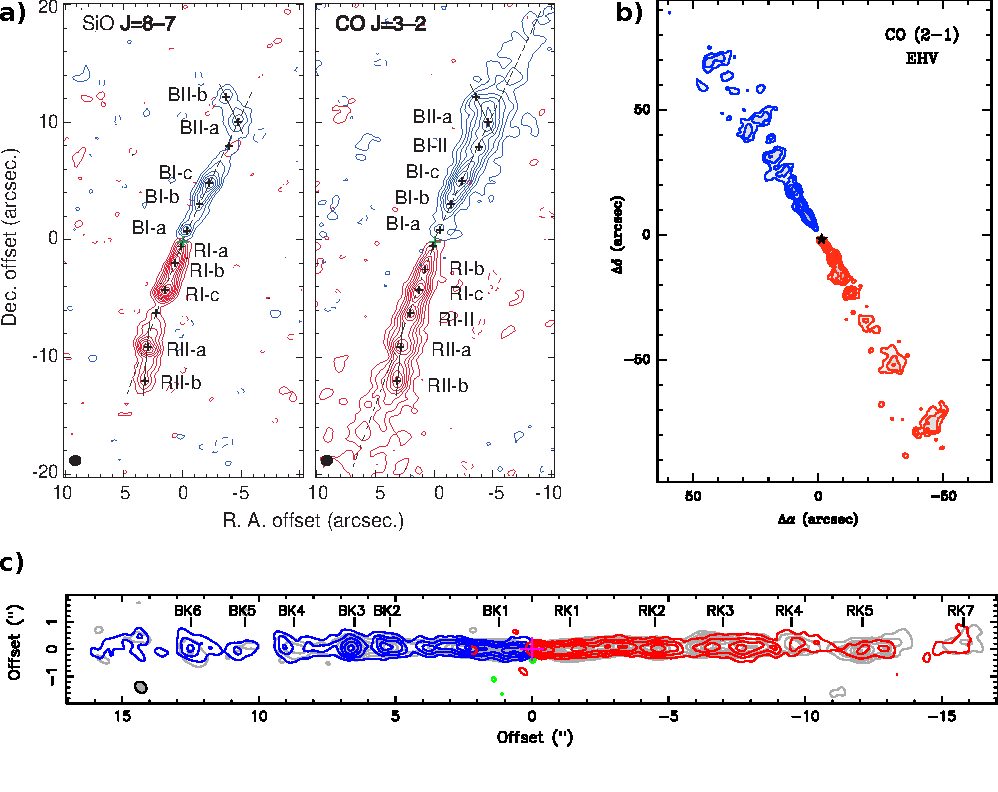
\includegraphics[width=\textwidth]{figures/molecularjets.pdf}
\caption[Molecular jets]{a) L1448C \citep{hirano2010}. b) IRAS04166 \citep{santiago-garcia2009}. c) HH211 \citep{lee2010, moraghan2016}}
	\end{center}
\end{figure}

\begin{deluxetable}{lccccccccc}
% \rotate
\tabletypesize{\footnotesize}
\tablewidth{0pt}
\tablecaption{\small Young stellar objects with molecular jets. \label{tab:molecularjets}}
%\tabletypesize{\scriptsize}
\tablehead{
\multicolumn{1}{l}{}       & \colhead{Class} & \colhead{Molecules} & \colhead{Distance} & \colhead{M$_*$}       & \colhead{$L_{\rm bol}$} & \colhead{v$_j$}    & \colhead{$\dot{M}_j$}           & \colhead{$\dot{M}_{\rm acc}$}   & \colhead{Refs.} \\ %[-0.9em]
\multicolumn{1}{l}{Source} & \colhead{}      & \colhead{}          & \colhead{(pc)}     & \colhead{(M$_\odot$)} & \colhead{(L$_\odot$)}   & \colhead{($\kms$)} & \colhead{(M$_\odot$ yr$^{-1}$)} & \colhead{(M$_\odot$ yr$^{-1}$)} & \colhead{}
} 
\startdata
L1448C          & \nodata & \nodata & \nodata & \nodata & \nodata & \nodata & \nodata & \nodata & \nodata \\
SVS~13          & \nodata & \nodata & \nodata & \nodata & \nodata & \nodata & \nodata & \nodata & \nodata \\
SVS~13B         & \nodata & \nodata & \nodata & \nodata & \nodata & \nodata & \nodata & \nodata & \nodata \\
L1157           & \nodata & \nodata & \nodata & \nodata & \nodata & \nodata & \nodata & \nodata & \nodata \\
HH211           & \nodata & \nodata & \nodata & \nodata & \nodata & \nodata & \nodata & \nodata & \nodata \\
HH212           & \nodata & \nodata & \nodata & \nodata & \nodata & \nodata & \nodata & \nodata & \nodata \\
HH111           & \nodata & \nodata & \nodata & \nodata & \nodata & \nodata & \nodata & \nodata & \nodata \\
Cep~E           & \nodata & \nodata & \nodata & \nodata & \nodata & \nodata & \nodata & \nodata & \nodata \\
IRAS~04166 :    & \nodata & \nodata & \nodata & \nodata & \nodata & \nodata & \nodata & \nodata & \nodata \\
IRAS4A2 & \nodata & \nodata & \nodata & \nodata & \nodata & \nodata & \nodata & \nodata & \nodata \\
IRAS~17233 & \nodata & \nodata & \nodata & \nodata & \nodata & \nodata & \nodata & \nodata & \nodata \\
C7              & \nodata & \nodata & \nodata & \nodata & \nodata & \nodata & \nodata & \nodata & \nodata \\
HH80-81         & \nodata & \nodata & \nodata & \nodata & \nodata & \nodata & \nodata & \nodata & \nodata \\
VLA 1624        & \nodata & \nodata & \nodata & \nodata & \nodata & \nodata & \nodata & \nodata & \nodata \\
SMM1-a          & \nodata & \nodata & \nodata & \nodata & \nodata & \nodata & \nodata & \nodata & \nodata \\
SMM1-b          & \nodata & \nodata & \nodata & \nodata & \nodata & \nodata & \nodata & \nodata & \nodata \\
Ser-emb8(N)    & \nodata & \nodata & \nodata & \nodata & \nodata & \nodata & \nodata & \nodata & \nodata \\
MMS5/OMC3     & \nodata & \nodata & \nodata & \nodata & \nodata & \nodata & \nodata & \nodata & \nodata \\
OMC2/FIR6b    & \nodata & \nodata & \nodata & \nodata & \nodata & \nodata & \nodata & \nodata & \nodata \\
B335            & \nodata & \nodata & \nodata & \nodata & \nodata & \nodata & \nodata & \nodata & \nodata \\
HOPS373?       & \nodata & \nodata & \nodata & \nodata & \nodata & \nodata & \nodata & \nodata & \nodata \\
\enddata
\\% [1em]
\tablecomments{Add some sources from \citep{podio2021} and \citep{dutta2023}. IRAS2A monopolar molecular jet? \citep{codella2014_IRAS2A}. Ser-emb 15 \citep{sato2023}.}
\tablerefs{
L1448C: \citet{bachiller1990}, \citet{hirano2010}, \citet{tafalla2010}, \citet{toledano-juarez2023}.
SVS~13: \citet{chen2016}, \citet{lefevre2017}, Blazquez-Calero et al. (submitted).
L1157: \citet{kwon2015}, \citet{james2020}.
HH211: \citet{gueth1999}, \citet{nisini2002}, \citet{hirano2006}, \citet{lee2009}, \citet{lee2010}, \citet{jhan2016}, \citet{moraghan2016}, \citet{jhan2021}. %\citet{ray2023}
HH212: \citet{codella2014_HH212}, \citet{lee2017}, \citet{lee2018_HH212}, \citet{lee2021}
HH 111: %\citet{cernicharo1996},
Cep~E: \citet{lefloch1996}, \citet{hatchell1999}, \citet{lefloch2015}, \citet{gomez-ruiz2015}, \citet{schutzer2022}.
I04166: \citet{tafalla2004}, \citet{santiago-garcia2009}, \citet{wang2014}, \citet{tafalla2017}, \citet{wang2019}.
NGC1333 IRAS4A2: \citet{choi2006}, \citet{choi2010}, \citet{choi2011}, \citet{ching2016}. % Do not mistake \citet{codella2014_IRAS2A} with IRAS4A2.
IRAS 17233-3606: \citet{leurini2009}.
C7: \citet{plunkett2015}.
\citet{hatchell1999}, \citet{lefloch2007}.
HH80-81:  \citet{qiu2009}, \citet{cheng2019}, \citet{qiu2019}.
VLA 1624: %\citet{andre90},
\citet{hara2021}.
SMM1-a: \citet{hull2016}, \citet{hull2017}, \citet{tychoniec2019}
SMM1-b: \citet{hull2016}, \citet{hull2017}, \citet{tychoniec2019}
Ser-emb 8(N): \citet{tychoniec2019}
% IRAS 03282+3035: \citet{bachiller1991}, \citet{tafalla1993}
% IRAS 2005+2720: \citet{bachiller1995}.
MMS 5/OMC-3: \citet{matsushita2019}.
OMC 2/FIR 6b: \citet{matsushita2021}.
B335: \citet{yen2010}, \citet{bjerkeli2019}.
HOPS 373: \citet{yoon2022}.
}
\end{deluxetable}

\section{Motivation of our work}

In this thesis \dots

\noindent
This thesis is structured as follows:

\chapter{Re50 radio jet}
\section{Introduction}
\section{Observations}
\section{Results}
\section{Analysis and discussion}
\section{Summary and conclusions}

\chapter{The SVS~13 system}
\section{The SVS~13 protobinary}

% SVS~13 is a YSO located in the NGC~1333 cloud, at a distance of $\sim 300$~pc \citep{ortiz-leon2018}. It is well known for being the proposed driving source of teh outstanding chane of HH objects HH~7-11. SVS~13 was discovered by \citet{strom1976} in the near-infrared, and at those time did not have a optically visible counterpart. \citet{eisloeffel1991} reported an outburst that occurred 1990$\pm$1, and the protostar have remained visible until then. 
% From VLA %3.6~cm 
% observations, \citet{anglada2000} revealed that it was a close (90~au in projection) binary system, with VLA~4A being the western component and VLA~4B the eastern one. It was later reported that only VLA~4B presents a stron 7~mm emission \citep{anglada2004}
% 
% SVS~13 is a young optically visible star \citep{eisloeffel1991} located in the NGC~1333 cloud, at a distance of $\sim 300$~pc \citep{ortiz-leon2018}. It is 
% 
% 
% Its components, VLA~4A and VLA 4B, being the B component located to the East \citep{anglada2000, anglada2004}, have a projected separation of $0\farcs3$ ($\sim 90$~au), and are surrounded by small protoplanetary disks \citep{2000ApJ...542L.123A, 2004ApJ...605L.137A}. VLA4 B is associated to the near-infrared variable source of SVS~13 \citep{2014ApJ...794..169H}. For this reason, to assign it an evolutionary stage is difficult, but it is often regarded as a young Class I or a Class 0/I transition source \citep{2000A&A...362L..33B, 2009ApJ...691.1729C}.  Also its variability does not seem to fit within a pure classification: the light curve in K-band photometry shares the long duration maximum with FU orionis type outbursts, while spectroscopically it resmbles an EXor star; and the small outburst amplitud resembles neither \citep{hodapp2014}.  
% 
Introduction to SVS~13. Young binary located in NGC1333. HH7-11 \citep{hartigan2019}. Palomar images. Outburst Eisloeffel. Protobinary discovery. 

\section{Two circumstellar disks and a circumbinary}
Two circumstellar disks and a circumbinary disk \citep{diaz-rodriguez2022} \citep{diaz-rodriguezphd}

\section{The SVS~13 outflow}
HH7-11, CARMA molecular outflow, H2 arcs and Fe jet, HST arcs, molecular bullets Bachiller and Chen. Lefevre. Radio jet.

\chapter{ALMA observations of SVS~13 outflow}

\section{Introduction}

Introduction to SVS~13. Young binary located in NGC1333. HH7-11 \citep{hartigan2019}. Large-scale molecular outflow. SVS~13 large scale outflow was between the first ones (the sixth), and was associated to the HHs \citep{snell1981}. Bullets. 
Two circumstellar disks and a circumbinary disk \citep{diaz-rodriguez2022} \citep{diaz-rodriguezphd}.


\section{Observations and data reduction}\label{sec:observations}

\begin{figure}[h!]
\begin{center}
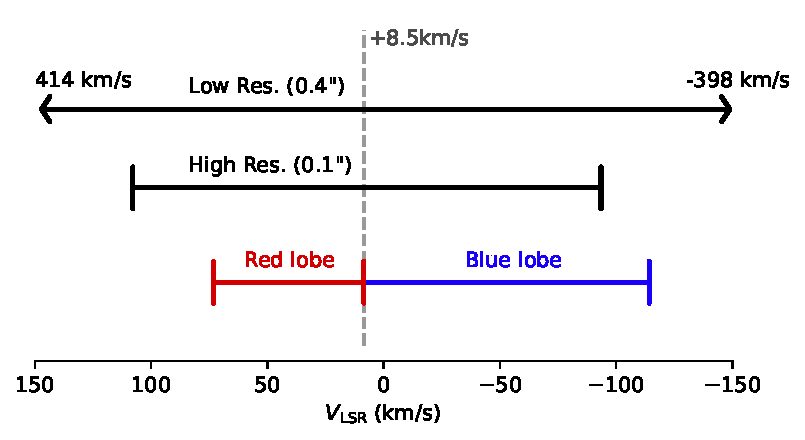
\includegraphics[width=1.0\textwidth]{figures/spectral_setup.pdf}\\
\caption[Spectral setup]{
	Graphical description of the spectral setup of the ALMA observations
\label{fig:spectralsetup}}
\end{center}
 \end{figure}



The CO($J$=3-2) ALMA observations were carried out in band 7 (0.9 mm), during Cycle 3 (program 2015.1.01229.S; PI: G. Anglada) and Cycle 4 (program 2016.1.101305.S; PI: G. Anglada). Here, we present a summary of the observations focused on the CO(3-2) data.


The Cycle 3 ALMA 12-m array observations were carried out during two runs on 2016 September 9 and 10, using 42 antennas with baselines in the range of 15-3225~m, providing an angular resolution of $\sim$$0\farcs1$ and a maximum recoverable scale of $\sim$$12''$ (strict upper limit, obtained from the shortest baseline) and of $\sim$$3''$ (good quality imaging, obtained from the $5^{\rm th}$ percentile shortest baseline). The channel width was 122~kHz, corresponding to 0.106~\kms\ at 345.795990~GHz, the assumed rest frequency of the CO($J$=3-2) transition. The total bandwidth was 234.375~MHz, covering an LSR velocity range from $-$93.32 to 109.47~\kms.

The Cycle 4 ALMA 12-m array data were obtained on 2016 November 24, using 43 antennas with baselines in the range of 15-704~m, providing an angular resolution of $\sim$0.4$\arcsec$ and a maximum recoverable scale of $\sim$$12''$ (from the shortest baseline) and of $\sim$$3''$ (from the $5^{\rm th}$ percentile baseline). The channel width was 244~kHz, corresponding to 0.211~\kms, and the total bandwidth was 937.500~MHz, covering an LSR velocity range from $-$398.34 to 414.25~\kms.

In both cycles, the calibrators J0237+2848, J0238+1636, and J0336+3218 were used for the 12-m array bandpass, absolute flux, and complex gain calibration, respectively.


Cycle 4 observations with the 7-m Atacama Compact Array (ACA) were carried out on 2016 November 15, and 2017 July 7 and 26, with an angular resolution of $\sim$4$\arcsec$ and a maximum recoverable scale of $\sim$$35''$. The channel width was 122~kHz (0.106~\kms) with a total bandwidth of $250$~MHz, covering an LSR velocity range from $-$100.00 to 116.64~\kms. The bandpass calibrator was J0510+1800 for the November 15 and July 7 observations, and J0522-3627 for the 26 July observations. The absolute flux calibrator was Ceres for the November 15 observations, and Uranus for the remaining observations. The complex gain calibrator was J0319+4130 for all the observations. 


The phase center of all the observations was set at RA(ICRS)=$03^\mathrm{h}29^\mathrm{m}03\fs75$, Dec(ICRS)=$31^\circ16\arcmin 04\farcs 00$, within $\sim$$0.3''$ of the position of VLA4B. The FWHM of the 12-m primary beam is 18$''$, and that of the 7-m array is 32$''$. The images presented in this paper have not been corrected by the primary beam response, except when indicated. 

The observations were pipeline calibrated using CASA versions 4.7.01 and 4.7.2, for Cycle 3 and 4, respectively. Additionally, the 12-m array Cycle 3 data (1.6~h on-source with $\sim 0.1\arcsec$ resolution) were phase self-calibrated. Self-calibration was unsuccessful for the Cycle 4 data (only 4.15~min on-source with $\sim 0.4''$ resolution). 


Because of the small primary beam of the ALMA 12-m array, only Bullet 1 has been imaged with these data. The larger size of the ACA primary beam allows us to detect Bullet 2 in CO($J$=3-2), but at low angular resolution (see Extended Data Fig.~9).


% \section{Two circumstellar disks and a circumbinary disk?}
% \citep{diaz-rodriguez2022} \citep{diaz-rodriguezphd}

\section{Results}

\subsection{Description of the molecular outflow}

\begin{figure}[h!]
\begin{center}
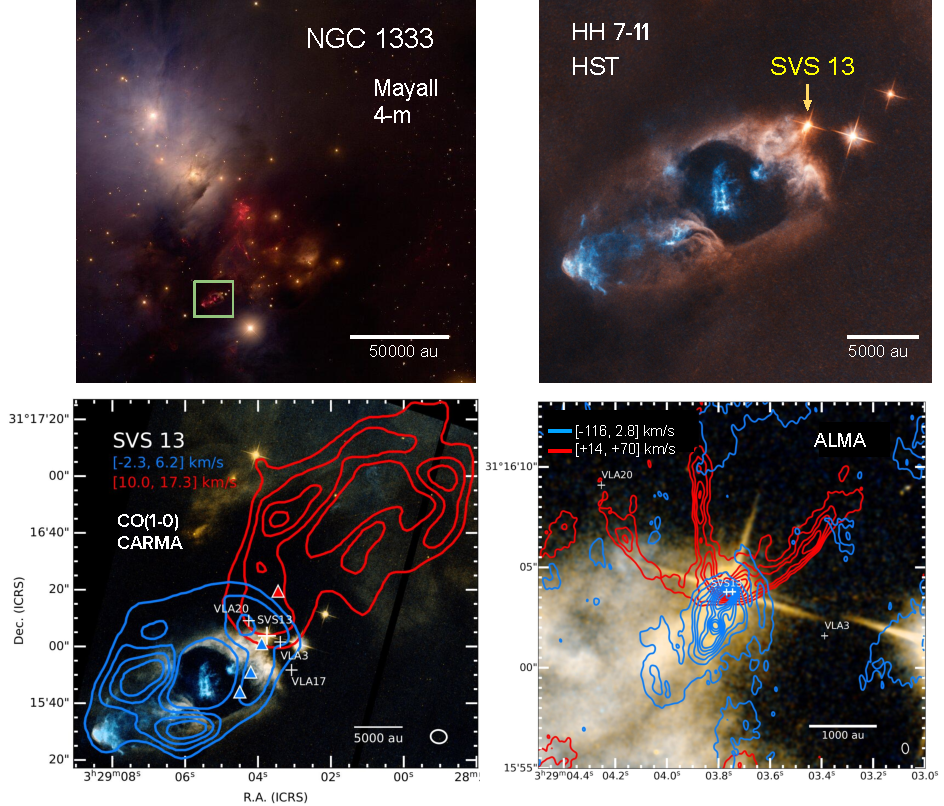
\includegraphics[width=1.0\textwidth]{figures/SVS13outflow.pdf}\\
\caption[SVS~13 outflow]{
	NGC1333, HH7-11, SVS~13 large-scale molecular outflow, ALMA view of the molecular outflow.
\label{fig:SVS13outflow}}
\end{center}
 \end{figure}



 Broad description of the outflow. Description of the blue and red lobes. Outflow cavities. EHV emission. Nebulosities?. Molecular bullet 1 and 2 with ACA. Rich substructure in bullet 1 with ALMA.

% \section{Kinematic substructure of the extremely high velocity gas}
% \section{Kinematic substructure of Bullet 1}
% \subsection{Morphological and kinematical substructure of the molecular jet}

\begin{figure}[p!]
\begin{center}
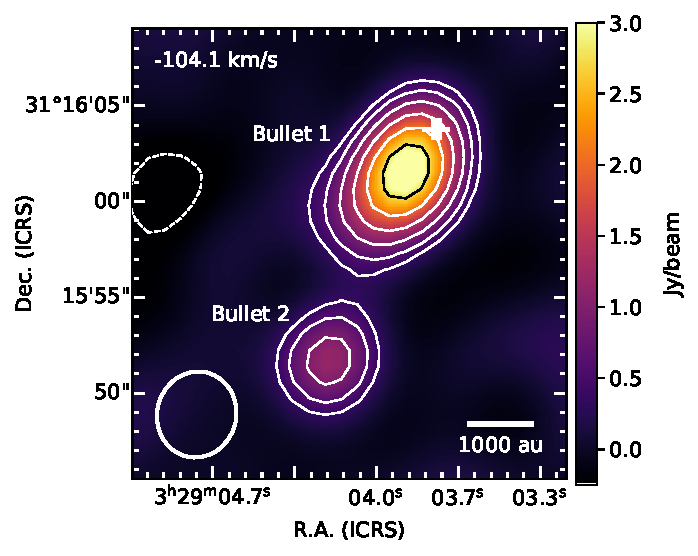
\includegraphics[width=\textwidth]{figures/bullet2aca.pdf} \\
\caption[Extended Data Fig.\ 9: Detection of Bullet 2 with ACA]{{\bf Extended Data Fig.\ 9: Detection of Bullet 2 with ACA.}
Image of the CO($J$=3-2) line emission of the blueshifted bullets 1 and 2 in SVS~13, obtained with the 7-m ACA array, at an LOS velocity of $-$104 km s$^{-1}$ relative to VLA~4B (v$_{\rm LSR}=$ +9.3~\kms)\cite{diaz-rodriguez2022}, where the emission of Bullet 2 peaks. The synthesized beam is $4\farcs51\times 4\farcs13$ (PA=$-13.90^\circ$), and the channel width is 0.44 \kms. Contour levels are -3, 3, 5, 8, 12, 17, 23, and 30 times 0.12 mJy~beam$^{-1}$, the rms of the map. The position of the SVS~13 binary is indicated with white plus signs. The image has not been corrected for the primary beam response. Bullet 2 appears unresolved in the ACA image, with a flux density is 1.9 Jy, after correction for the primary beam response. This second bullet is not detected with the ALMA 12-m array because of a lack of sensitivity at the distances where it is located, due to the smaller size of the 12-m array primary beam. The second bullet was previously detected only at longer wavelengths \cite{bachiller2000,chen2016,lefevre2017}. 
\label{fig:bullet2aca}
}
\end{center}
\end{figure}


\subsection{Substructure of the molecular jet}


\begin{figure}[p!]
\begin{center}
 %\includegraphics[width=1.0\textwidth]{figures/fig3.pdf}
 %\includegraphics[width=1.0\textwidth]{figures/moments_all.jpg}
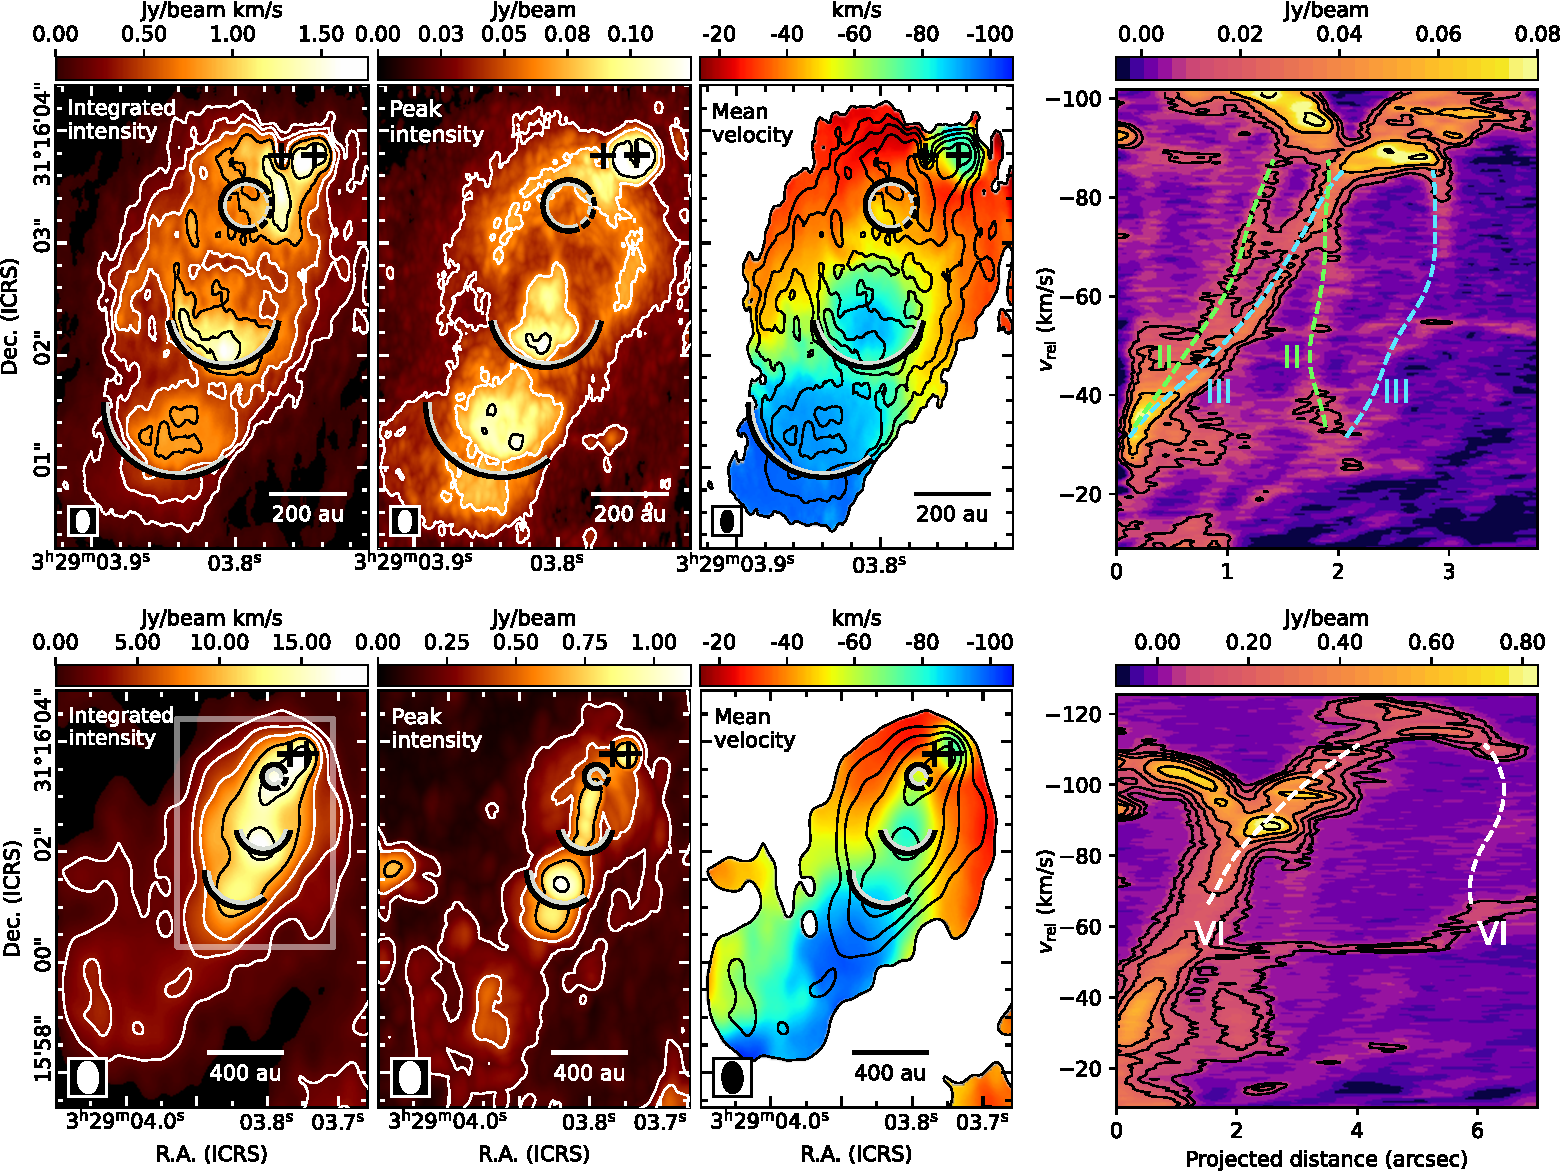
\includegraphics[width=\textwidth]{figures/moments.pdf}
\end{center}
 \end{figure}
%\clearpage
%\addtocounter{figure}{-1}
\begin{figure}[p!]
\begin{center}
 %\includegraphics[width=1.0\textwidth]{figures/fig3.pdf}
 %\includegraphics[width=1.0\textwidth]{figures/moments_all.jpg}
\caption[Figure 1 name]{
{\bf Observed CO($J$=3-2) images and position-velocity diagrams of the blueshifted Bullet 1 in SVS~13.}
{Panels in the top row have been obtained from the high-angular resolution ALMA CO($J$=3-2) data (beam = $0\farcs173 \times 0\farcs091$, PA = $-2.2^\circ$) covering the velocity range from $-$9.3 to $-$102.7~\kms. Panels in the bottom row have been obtained from lower angular resolution ALMA data (beam = $0\farcs527 \times 0\farcs333$, PA = $2.7^\circ$) that cover a wider velocity range, from $-$9.3 to $-$126.4~\kms. {\bf First column:} Images of the velocity-integrated intensity (zeroth-order moment of the spectral cube). Contour levels are 3, 6, 10, 16 and 25 times $0.05$ Jy~beam~$^{-1}$ \kms\ (top) and $0.61$ Jy~beam$^{-1}$~\kms\ (bottom). {\bf Second column:} Images of the peak intensity of the spectral cubes. Contour levels are 3, 6, 10, and 16 times $0.011$ Jy~beam$^{-1}$ (top) and $0.066$ Jy~beam$^{-1}$ (bottom).  {\bf Third column:} Images of the mean velocity field (first-order moment, or intensity-weighted average velocity), in color scale, overlaid on the integrated intensity (in contours).  {\bf Fourth column:} Position-velocity diagrams (width = $0.1''$ and $0.4''$ for top and bottom panels, respectively) along the longitudinal axis of the bullet ($\mathrm{PA}=160^\circ$), and origin in VLA~4B, with the emission of the families of rings II, III, and VI (defined in Fig.~\ref{fig:ellipses}) indicated with green and cyan (top row) and white (bottom row) dashed lines, respectively. Contour levels are 5, 10, 20, 35, 60 and 90 times 
 %the rms (0.0025 Jy~beam$^{-1}$ and 0.010 Jy~beam$^{-1}$ respectively for the top and bottom panels).
 0.0025 Jy~beam$^{-1}$ (top) and 0.010 Jy~beam$^{-1}$ (bottom).
The positions of the two protostars of the SVS~13 binary, VLA~4A (west) and VLA~4B (east), near the top right corner of the images, are indicated by plus signs. 
All velocities are LOS velocities relative to that of VLA~4B ($V_{\rm LSR}$ = +9.3 \kms). The images have been corrected by the decrease in sensitivity due to the primary beam response. For the high-resolution data (top images) a clipping of 14 mJy beam$^{-1}$ (4-$\sigma$ before primary beam correction) has been applied to the individual channel maps (with the native channel width of 0.106~\kms) before constructing the moments. 
The H$_2$ arcuate features are plotted as arcs using double, black and white, lines for better visibility; their positions have been obtained from the infrared images, adopting the Gaia coordinates for the star ($\sim 0.07\arcsec$ south-east from the radio position of VLA 4B), and correcting for the estimated proper motions of the arcs relative to the star.
Synthesized beams are plotted as ellipses at the bottom left corner of the images.
 \label{fig:mom}}}%Figure 1
\end{center}
 \end{figure}






{\color{blue}
Moments. Correspondance of the maxima with the arcs of Hodapp. Channel maps. Identification of the observed line emissionas CO.
}

  The velocity centroid map (third column in Fig.~\ref{fig:mom}) shows a clear apparent acceleration with distance from SVS~13, confirming previous lower resolution results. The velocity field is roughly symmetric with respect to the jet axis. This is in contrast with early claims for large transverse velocity gradients which probably resulted from an insufficient angular resolution and/or centroid calculation over very specific velocity ranges.
 % 
   A more revealing and striking view of the kinematics is obtained by looking at individual line channels in the CO($J$=3-2) image cube (see Fig.~\ref{fig:channels}, Extended Data Fig.\ 1, Supplementary Figs.\ 1 and 2, and Supplementary Videos 1 and 2). The channel images (specially the data of $\sim$$0.1''$ = 30 au resolution) show several sequences of rings whose positions and sizes change smoothly as a function of the line-of-sight (LOS) velocity. The rings are narrow, until they abruptly transform into a bright filled circle that we call the ``head''. We call each of these sequences of rings (and its head) a ``family''. The rings are detected at LOS velocities from approximately $-$9 to $-$125~\kms\ relative to the cloud, have radii in the range $0\farcs2$ to $2\farcs5$ (60 to 750 au) and extend southeast up to $\sim$$5''$ ($\sim$1500 au), in projection, from SVS~13. In general, the brightest part of a ring is that closest in projection to SVS~13 and, in some cases, the rings appear incomplete, as arcs.
 % 
  Assuming that the heads of the families are moving approximately along the symmetry axis, at an inclination angle $i=25^\circ$ (except for Rings I, for which we assume $i=22^\circ$) (see Methods), we can estimate their dynamical times from the ratio of their deprojected positions and mean velocities. We obtain dynamical times of $25\pm5$, $56\pm6$, $91\pm9$, $100\pm9$, and $134\pm15$~yr for families I-IV and VI, respectively (see bottom right panels of Fig.~\ref{fig:ellipses}). For family V, the head is not identified in our data and we obtain an upper limit of 102~yr from the positions and velocities of the rings. The typical separation in dynamical time between consecutive families is a few tens of years, suggesting a relationship with episodic mass ejection events separated this timescale. Interestingly, the epoch of the most recent ejection (family I, associated with a change in the orientation of the outflow) is 1992$\pm$5, 
  consistent with the epoch of the strong optical/infrared outburst of the visible component of SVS~13 (VLA~4B), which occurred in 1990$\pm1$, suggesting an association between these phenomena. To our knowledge, this is the first time that such a close association between an optical/infrared outburst and an EHV molecular bullet has been demonstrated.
 % 
 % 
  To illustrate the direction changes in the SVS~13 outflow, we plot in the bottom right panels of Fig.~\ref{fig:ellipses} the PA relative to VLA~4B, measured at the head of each family, as a function of the estimated dynamical time.
 % We note a quick jump in PA, from $\sim$160$^\circ$ to $\sim$140$^\circ$ in only 30 yr, in the most recent ejection (the one associated with family I and the optical/infrared outburst). This is in contrast to the previous stability of the PA at $\sim$160$^\circ$ over longer periods of $\sim$80 yr (between families I to VI and H$_2$ arcs 2-3, and between Bullets 2 and 3). This unusual pattern of PA changes suggests either twin jets from a yet unresolved close binary in VLA~4B or abrupt disk reorientations during some outbursts. This complex issue will be further discussed in a dedicated future paper.

 Families of rings.

Ellipse fitting. %\label{sec:ellfit}

The ellipse fitting to the rings in the channel maps has been carried out using an interactive program written in Python. This program finds the geometrical parameters (center coordinates, semimajor-axis, ellipticity, and PA) that maximize the mean intensity that falls within an elliptical annulus (we chose a width of a few pixels, $\sim$1/3 of the beam size). The program takes as initial guess the geometrical parameters of an ellipse that visually fits a targeted ring, calls the function ``minimize'' from the Python's package {\sc SciPy}, and returns the best-fit parameters. The fitting method L-BFGS-B was chosen, which allows bound-constrained minimizations. It is crucial to constrain the parameter-space to ensure that the fitting is performed to the targeted ring of a given family. In this manner, we avoid that additional emission affects the fit, whether the additional emission comes from a ring of a different family or from other kind of structure. 

 %We note that, when two rings of different families intersect in a given channel map, the inner region common to both rings often appears enclosed within the arcs (one of each ring) that connect the two intersection points of the rings (see the middle row of panels in Fig. 2????); these connected arcs simulate a (false) third ring, which must be excluded from the fit.
We note that, when two rings of different families intersect in a given channel map, the inner region common to both rings often appears enclosed within the arcs (one from each ring) that connect the intersection points (see the middle row of panels in Fig.~\ref{fig:channels}); these connected arcs simulate a (fake) third small ring, which must be excluded from the fit.
 %We note that, when two rings of different families overlap in a given channel map, the inner region common to both rings often appears enclosed within the two arcs (one of each ring) that connect the two points of intersection of the rings (see central row of panels in Fig. 2???); this simulates a third (fake) ring, which must be excluded from the fit.
 %We note that, when two rings of different families overlap in a given channel map, the arcs (one from each ring) bounded by the two points of intersection surround the inner region common to both rings, simulating a third (fake) ring (see central row of panels in Fig. 2???), which must be excluded from the fit.
%We note that, when two rings associated with different families intersect in a channel map, a third smaller ring arises, which should be excluded from the fitting.
 %(see, for example, the channel with velocity $-35.64$~\kms\ of Figure~\ref{fig:channel_selection}).
This means that the classification of rings into families has to be performed previously to the fitting, once it is clear which are the true rings that should be fitted.
 %and which are interpreted as the results of an intersection of rings from different families.
To better ensure the correct identification of rings in families, we perform the fitting on a channel by channel basis, using as initial parameters the solution of the previous channel fit. This usually gives good solutions, since the rings of a given family vary smoothly with velocity. We note that the elliptical fits of the heads of the families, which appear as filled emission, are visual estimates.

In Supplementary Figs.~1 and 2 we present the whole set of channel maps, with the elliptical fits superimposed on the rings (see also Supplementary Video 3, where we show how the elliptical fits change with the channel maps).


% \clearpage
\begin{figure}[p!]
\begin{center}
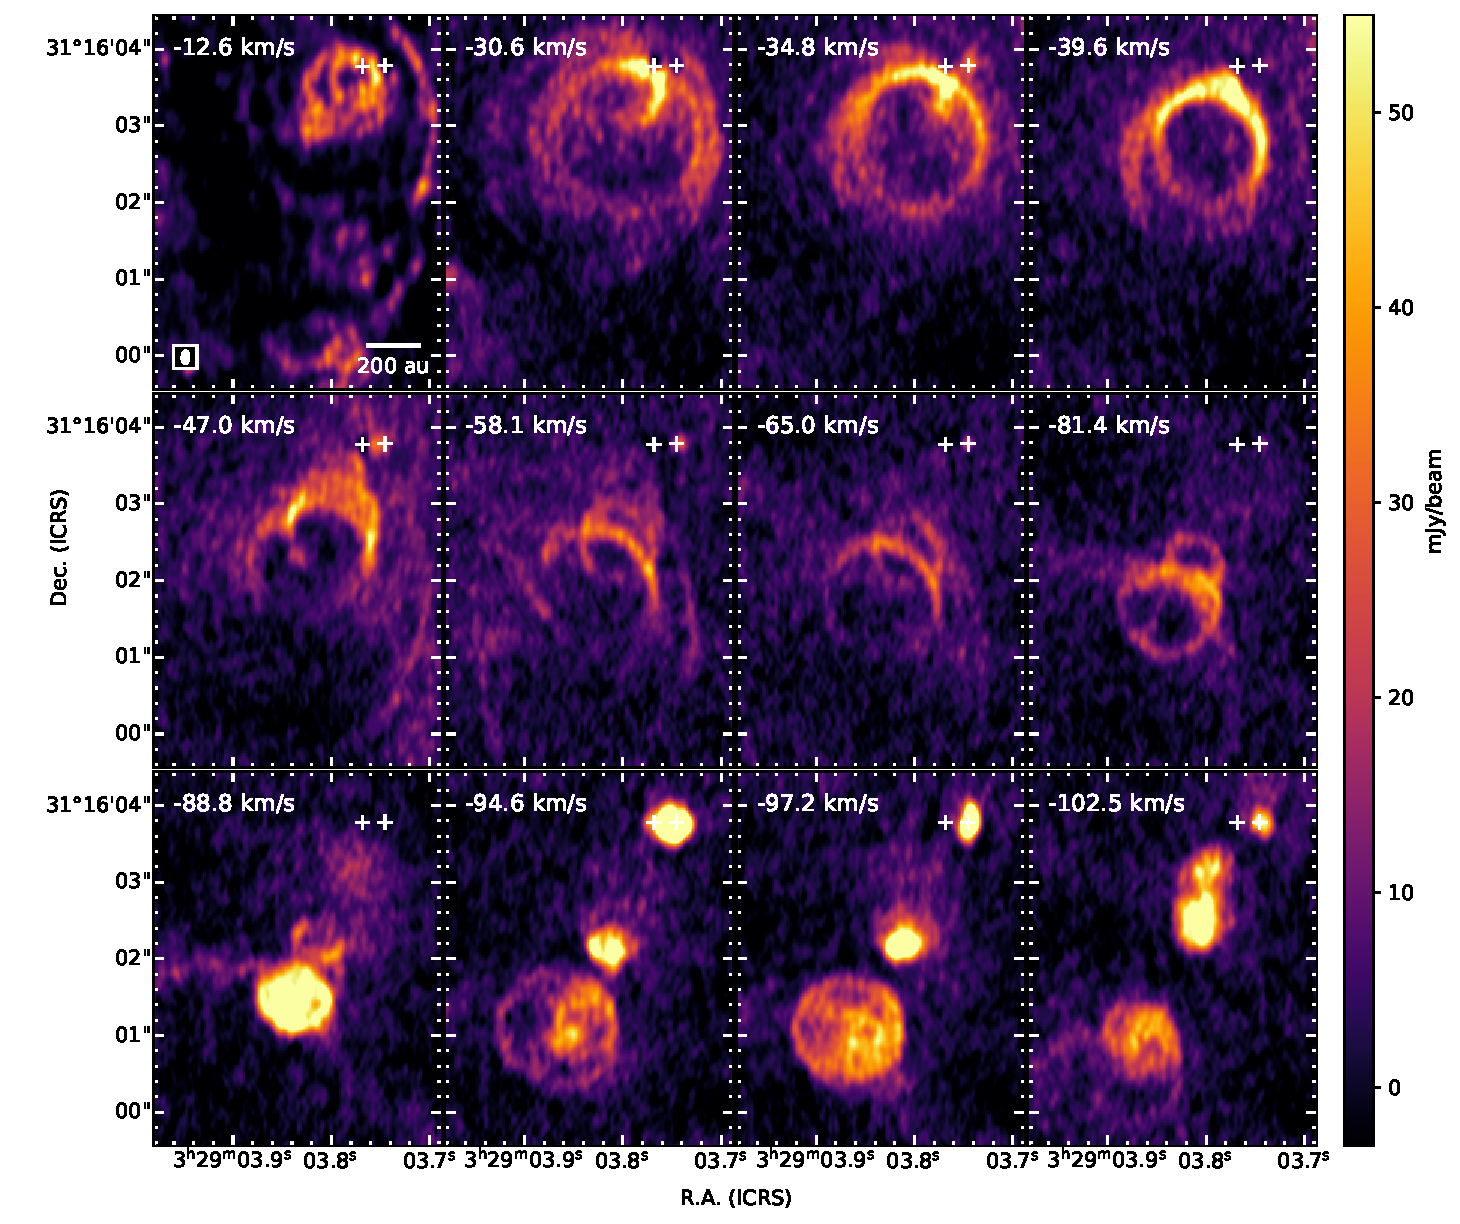
\includegraphics[width=1.0\textwidth]{figures/channels_hr.pdf}\\
\caption[Selection of high resolution channel maps]{
Observed CO($J$=3-2) spectral channel images at high angular resolution. A sample of high angular resolution channel maps of the CO($J$=3-2) emission observed by ALMA, which illustrate the ringed kinematic structure of the bullet. The synthesized beam is $0\farcs173 \times 0\farcs091$ (PA = $-2.2^\circ$), and is plotted as an ellipse in the bottom left corner of the first image. The full set of observed channel maps is shown in Supplementary Fig.~1 and Supplementary Video~1.
The positions of the two protostars of the SVS~13 binary
 are indicated by plus signs. The LOS velocity relative to VLA~4B is shown in the top left corner of each image. The width of each of the channels shown in the figure is 0.53~\kms, which corresponds to the average of five native channels. The rms of the images is 2.6 mJy beam$^{-1}$. Images have not been corrected by the primary beam response.
Lower angular resolution channel maps, covering a wider range of velocities, are shown in Extended Data Fig.~1, Supplementary Fig.~2 and Supplementary Video~2. 
\label{fig:channels}}%Figure 2
\end{center}
 \end{figure}



\begin{figure}[p!] 
\begin{center}
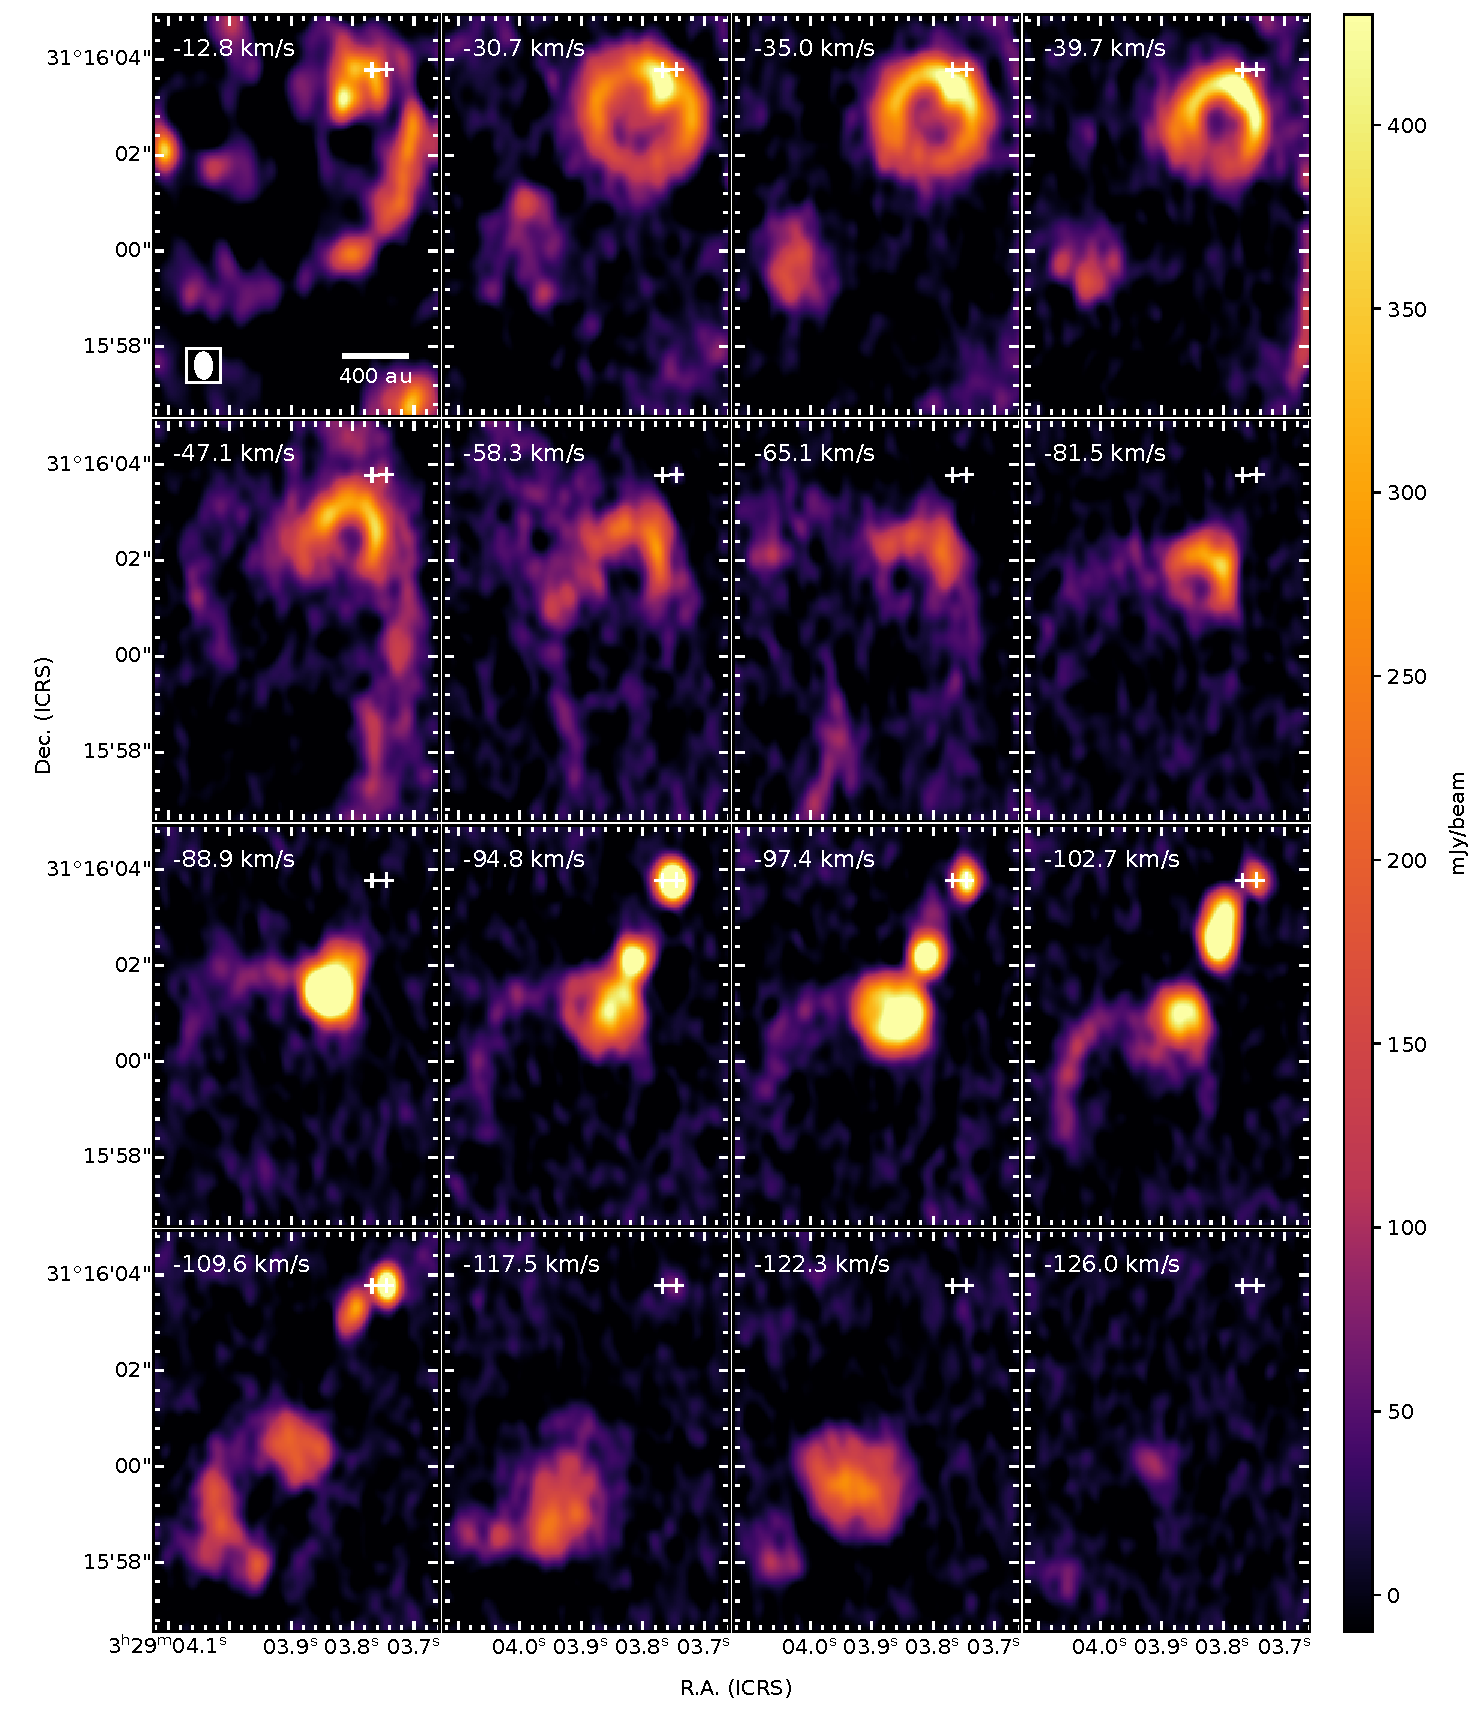
\includegraphics[width=0.90\textwidth]{figures/channels_lr.pdf}\\
\caption[Selection of high resolution channel maps]{
Observed CO spectral channel images of Bullet 1 at low angular resolution. A sample of spectral channel images of the CO($J$=3-2) emission observed by ALMA with a synthesized beam of $0\farcs527 \times 0\farcs333$ (PA = 2.7$^\circ$). The obtained data cover a range of velocities wider than the high angular resolution data shown in Fig.~\ref{fig:channels}. The positions of the two protostars of the SVS~13 binary \citep{anglada2000} are indicated by plus signs. The LOS velocity, relative to the velocity of VLA~4B \citep[$V_{\rm LSR}$ = +9.3 \kms;][]{diaz-rodriguez2022}, is shown in the top left corner of each image. The width of each of the spectral channels is 0.53 \kms. The rms of the images is 10 mJy beam$^{-1}$. Images have not been corrected by the primary beam response. The synthesized beam is plotted as an ellipse in the bottom left corner of the first image.
 \label{fig:lowres}}
 \end{center}
\end{figure}




\subsection{Families of rings}

\begin{figure*}[p!] 
\begin{center}
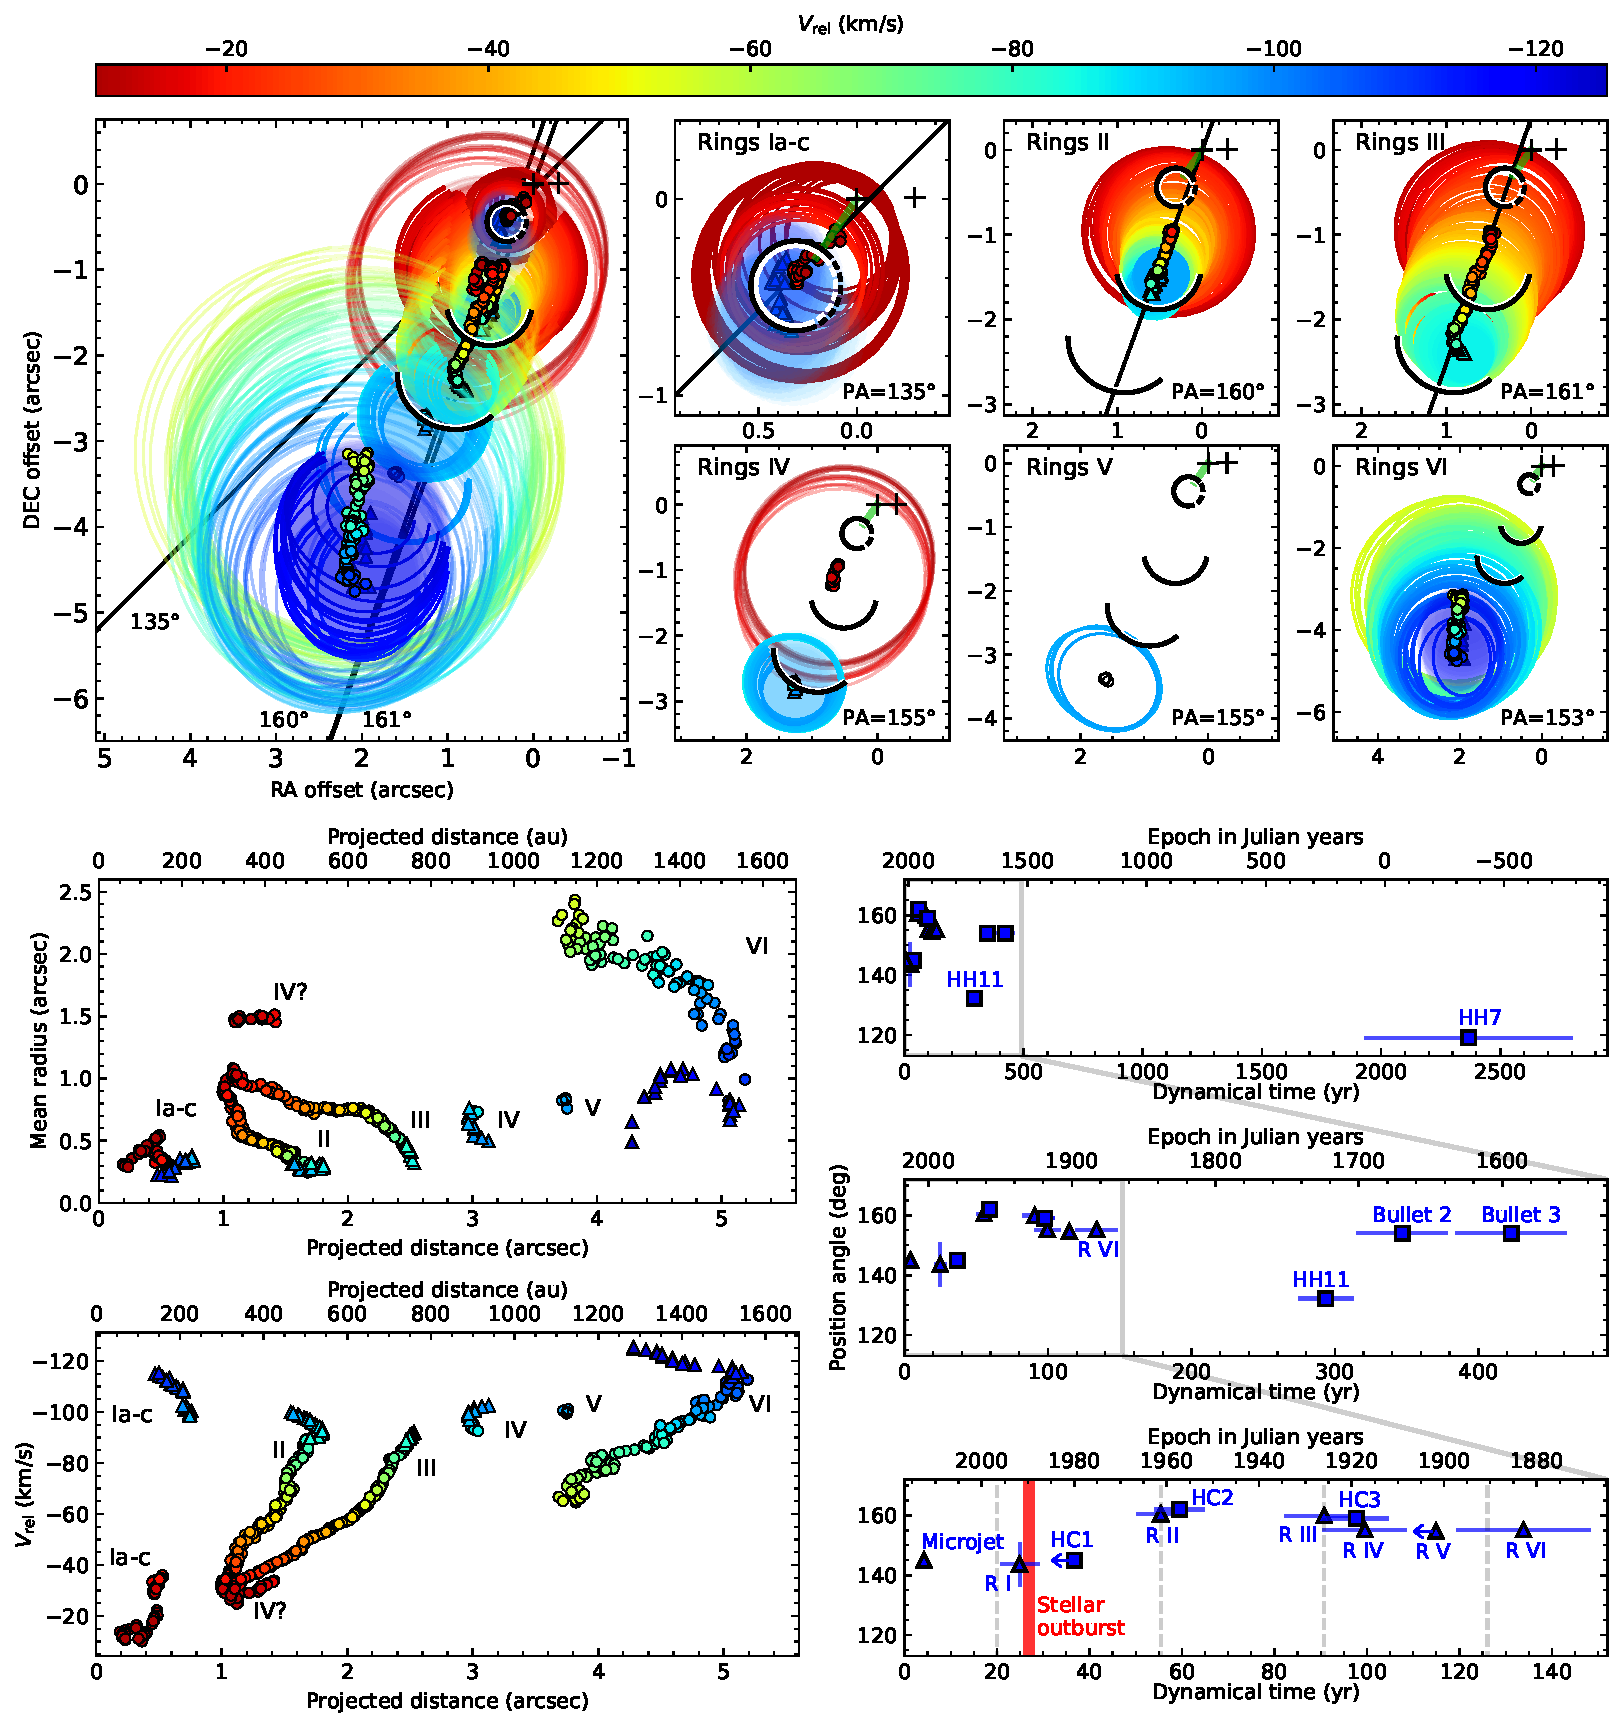
\includegraphics[width=1\textwidth]{figures/ellipsefits.pdf}
%\caption{~
%\label{fig:ellipses}%}%Figure 3
\end{center}
\end{figure*}

\begin{figure}[p!]
\clearpage
\noindent
\caption[Figure 3 name]{{\bf Decomposition of the ringed emission through elliptical fits.} 
{\bf Top left panel:} Color-coded plot of elliptical fits to the observed CO($J$=3-2) spectral channel images (see Methods for fitting procedure). Rings are represented by the ellipses that best-fit their emission, and filled emission regions are represented by shaded areas. 
Some ellipses have been drawn with increased transparency to improve the visualization. 
Color dots and triangles indicate the centers of the rings and of the regions of filled emission, respectively. The color represents the LOS velocity relative to VLA~4B. We note a trend of the rings to group in sequences that we call ``families''. In each family, the absolute value of the velocity of the rings increases and their size decreases with distance to the stars (indicated as black plus signs), ending in a filled region of emission (the ``head''). Several ``families'' of rings (labeled I to VI) are identified. The centers of the rings in each family appear rather well aligned, and linear regression fits to these positions for families I, II, and III are plotted as black
 %(dashed?)
 {\bf Top right panels:} Separate plots of each of the identified families of rings.
 The green segment in the
 %OJO!!!!plot of family I represents 
 {\bf Bottom left panels:} Plots of the mean radius (mean of the semimajor and semiminor axes of the ellipses) and the LOS velocity of the fitted rings, as a function of the distance (projected on the plane of the sky) of their centers to VLA~4B. The plots illustrate the general trends (except for the heads) for the radius to decrease with distance, and for the velocity to linearly increase with distance (a ``Hubble-Lema\^itre type'' law). The different families of rings are easily identified in the plots.
 %(PARA LOS RINGS I QUIZAS SE NECESITE VLA4A??? OJO: ES SIMPLEMENTE LA DISTANCIA DEL CENTRO A VLA4B, CADA PUNTO CON SU PA, O LA DISTANCIA MEDIDA A LO LARGO DE UN CIERTO PA, EL MISMO PARA TODAS?)
%(defined as the position that we expect corresponds to the more distant point; in practice, the position with the brightest emission in the channel images of filled-in emission, intermediate to the points that show the largest projected distance and the highest velocity).
 {\bf Bottom right panels:} PA as a function of the dynamical time for the heads of the families of rings (plotted as triangles and labeled R I to R VI; see Methods for details on the calculations), as well as for other features associated with the SVS~13 outflow, such as HH objects (plotted as squares and labeled HH7, HH11), [FeII] jet (triangle labeled as Microjet), and H$_2$ arcs (squares labeled as HC1, HC2, HC3). We assumed inclination angles from $22^\circ$ to $25^\circ$ (see Methods). 
 Epoch is given in Julian years, with epoch 2000 corresponding to the standard definition of Julian epoch J2000.0. Dynamical times are relative to the date of our high-angular resolution ALMA observations (epoch 2016.69).
\label{fig:ellipses}
 }
\end{figure}



\section{Analysis and discussion}

\subsection[Identification of the observed line emission as CO at EHV]{Identification of the observed line emission as CO at extremely high velocities.}
% 
\begin{figure}[p!] 
\begin{center}
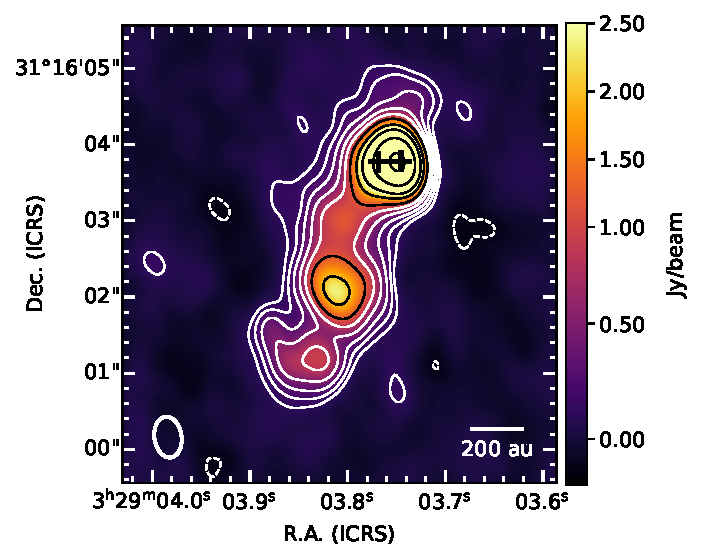
\includegraphics[width=\textwidth]{figures/SO.pdf}\\
\caption[Observed SO image of Bullet 1]{{\bf Observed SO image of Bullet 1.}
Image of the velocity-integrated intensity of the SO(8$_8$-7$_7$) line observed with the ALMA 12-m array using a low spectral resolution spectral window dedicated to continuum observation, with a channel spacing of 13.6~\kms. The emission has been integrated in the LOS velocity range from $-$9.8 to $-$118.6~\kms\ relative to the velocity of VLA 4B ($+$9.3~\kms). The positions of the two protostars of the SVS~13 binary \citep{anglada2000} are indicated by plus signs. The synthesized beam, shown in the bottom left corner, is $0\farcs54 \times 0\farcs36$ (PA = $8.37^\circ$). Contours are $-$3, 3, 5, 8, 13, 20, 30, 50, 80, 140, 260 times 0.04 Jy~beam$^{-1}~\kms$. The image has not been corrected by the primary beam response.
}
\end{center}
\end{figure}


 It is known that there is line emission associated with the SVS~13 disks corresponding to transitions of other molecular species, with different rest frequencies. For several of these transitions the difference in frequency with respect to the CO($J$=3-2) transition is similar to the Doppler shift corresponding to the range of velocities observed in the bullet. Therefore, in principle, it could occur that the emission that we attribute to EHV blueshifted CO in the bullet is indeed emission from other molecular transitions with higher rest frequencies arising from material moving at much lower velocities. We argue that this is not the case. Since CO is the most abundant detectable molecule, if the emission observed in some channels corresponds to other molecules, then we would expect to detect a CO ``replica'' of this emission in the velocity channels corresponding to the difference in frequency with respect to CO, which is not observed.
% 
 In addition, we identified SO($8_8$-$7_7$) emission in the bullet from a spectral window dedicated to continuum observations, with a low spectral resolution of 27.2~\kms. Considering the rest frequency of this transition, 344.310612~GHz, the emission reaches velocities about $-$120~\kms\ (relative to the LSR velocity of VLA~4B), the same as the CO in the bullet. In Figure Extended Data Fig.\ 2, we show the integrated SO emission in the bullet. With a spatial resolution of $0\farcs54 \times 0\farcs36$, we can distinguish the main morphological substructure we found in the CO channel maps. Thus, we confirm that the main substructure observed in the bullet is traced by different molecular transitions, and that the substructure reported in the CO does not arise from the overlapping of different molecular lines in the same channel maps.
 Moreover, the main kinematical features of the bullet we have observed in CO(3-2) were already present, with the same velocities, in (lower resolution) CO(2-1) data, as well as in other molecular transitions, such as SiO(5-4) and SO($6_5$-$5_4$) lines. This coincidence in velocity is obviously highly unlikely if it were just the result of contamination from other species.


\subsection{Inclination angle}

From the high-angular resolution H$_2$ S(1) results\citep{hodapp2014} we can obtain a rough estimate of the inclination angle of the flow with respect to the LOS. For the farthermost H$_2$ arc (HC3), a proper motion of $\sim$30~\masyr\ ($\sim$43~\kms) relative to VLA~4B was measured\citep{hodapp2014}. This arc is positionally associated with the head of family III, that has a LOS velocity of $-$90~\kms\ relative to the velocity of VLA~4B ($V_{\rm LSR}$ = +9.3~\kms)\citep{diaz-rodriguez2022}. Thus, combining
the proper motion of this H$_2$ arc and the LOS velocity of the head, we obtain an inclination angle $i=25^\circ\pm2^\circ$. However, a proper motion for the second H$_2$ arc (HC2) could not be measured by \citet{hodapp2014}, so we derive its dynamical time assuming the same proper motion as HC3. Combining proper motion and LOS velocities, an inclination angle $i=22^\circ\pm3^\circ$ for the H$_2$ bubble (HC1) and the [FeII] jet was inferred~\citep{hodapp2014}. Since HC1 is positionally associated with the head of family I, we assume the same inclination angle of $22^\circ\pm3^\circ$ for this family. Moreover, inclination angles of $i=24^\circ\pm2^\circ$ for the Herbig-Haro object HH~11 and $i=25^\circ\pm5^\circ$ for HH~7C (a substructure of HH~7) were reported \citep{hartigan2019}. Thus, in order to estimate the dynamical times of the outflow features of SVS~13 (see bottom right panels in Fig.~\ref{fig:ellipses}), we have adopted the inclination angles determined 
 %for the objects listed
above.
 %, and an inclination angle of $25\pm2^\circ$ for those objects whose inclination angles are unknown. 
We note that the range of inclination angles mentioned above is compatible with our independent estimate of $i\simeq20^\circ$ obtained from our bowshock modeling (see ``Bowshock model'' section below in these Methods).

% We note that this inclination angle is similar to the one reported by \citet{hodapp2014} for the H$_2$ bubble closest to SVS13, about $22^\circ$ if a distance to the source of 300~pc is assumed.

% The position of the head of a family has been measured as the approximate location of the maximum emission in images of the peak intensity of the spectrum. 

% \subsection{Dynamical times of the heads and coincidence with a optical/infrared outburst}

\subsection{Dynamical times of the heads of the ring families}


We have obtained the dynamical times of the heads of the families of rings (see bottom right panel in Fig.~\ref{fig:ellipses}), assuming they have traveled with constant velocity in a straight direction along the jet axis, so
\begin{equation}\label{eq:thead}
	%t_\mathrm{dyn, {\rm head}}=x'_{\rm head}/(v_{z',\mathrm{head}}\tan i), \\
	t_{\rm head}=\frac{x'_{\rm head}}{v'_{\rm head}\tan i},
\end{equation}
where $x'_{\rm head}$ is the projected distance (on the plane of the sky) from the source to the head, $v'_{\rm head}$ is its LOS velocity relative to VLA 4B, and $i$ is the inclination angle of the flow with respect to the LOS (we use $i=22^\circ\pm2^\circ$ for Rings I and $i=25^\circ\pm2^\circ$ for the rest of the families, see ``On the inclination angle'' section in Methods). Both $x'_{\rm head}$ and $v'_{\rm head}$ are obtained by locating the maximum emission of each family of rings. For this, we first obtain several
 %(from 3 to 6)
 estimates of $x'_{\rm head}$ by locating the positions of the local maxima of emission near the jet axis in the peak intensity images (see second column of Fig~\ref{fig:mom}). Toward each of these positions we obtain spectra within a box with size of the order of the synthesized beam, and take $v'_{\rm head}$ as the LOS velocity of the emission peak. We then estimate the dynamical time of the head, $t_{\rm head}$, as the mean value of the dynamical times calculated using every measured pair of $x'_{\rm head}$ and $v'_{\rm head}$ values. The standard deviation of the dynamical times obtained in this way for a given head is of a few years (as indicated in the error bars of the bottom right panel of Fig.~\ref{fig:ellipses}). 

Using this procedure, we obtain dynamical times $t_{\rm head}$ = 25$\pm$5, 56$\pm$6, 91$\pm$9, 100$\pm$9, $<$102, and 134$\pm$15~yr, for ring families I to VI, respectively. We note that we could not find a clear maximum associated with the rings V head, which is expected to be located somewhere between the positions of rings IV and rings VI, but in a velocity range only available in the lower resolution images. Hence, we give only an upper limit for the dynamical time of rings V, obtained by substituting $x'_{\rm head}$ and $v'_{\rm head}$ in equation (\ref{eq:thead}) by the central position and 
 %relative
 the LOS velocity, respectively, of the ring observed in the highest velocity channel map of our high-angular resolution data.

%Therefore, we give only an upper limit for the dynamical time of the rings V, obtained by substituting in equation 5 x' and v' by the central position and relative LOS velocity, respectively, of the ring observed in the highest velocity channel map of our high angular resolution data.

% How we did it with rings I: Low resolution and high resolution.
% The kinematical times of the heads are interpreted differently For the rest of the rings, model dependent.
% Brief description of nebulosities? Rest of the objects

\subsection{Association of a molecular bullet with an optical/infrared outburst}

\subsection{Excitation temperature}

An estimate of the excitation temperature can be obtained from the observation of two rotational molecular transitions, $J$$\rightarrow$$J$$-$1 and $J'$$\rightarrow$$J'$$-$1. From Boltzmann's equation, and using equations (\ref{eq:tau1}) and (\ref{eq:dNJ}) to obtain the ratio of populations between the $J$ and $J'$ levels, we get:
\begin{equation}
 \frac{J'} {J} \, 
 \frac{e^{h\nu_{J',J'-1}/k_B T_\mathrm{ex}}-1} {e^{h\nu_{J,J-1}/k_B T_\mathrm{ex}}-1} \, 
 \frac{\ln{\left\{1- \frac{I_\nu(J\rightarrow J-1,\, v_{z'})}
{f_b \left[B_\nu(\nu_{J,J-1},\, T_\mathrm{ex}) - B_\nu(\nu_{J,J-1},\, T_{\rm bg})\right]} \right\}}}
%%{f_{J,J-1} \left[B_{J,J-1} (T_\mathrm{ex})-B_{J,J-1} (T_{\rm bg})\right]} \right\}}}
 {\ln{\left\{1- \frac{I_\nu(J'\rightarrow J'-1,\, v_{z'})}
{f'_b \left[B_\nu(\nu_{J',J'-1}, \, T_\mathrm{ex})-B_\nu(\nu_{J',J'-1}, \, T_{\rm bg})\right]} \right\}}}
%%{f_{J',J'-1} \left[B_{J',J'-1} (T_\mathrm{ex}) - B_{J',J'-1} (T_{\rm bg}) \right]} \right\}}}
 = e^{-(E_J-E_{J'})/k_B T_\mathrm{ex}},
\label{eq:Jratio3}
\end{equation}
where $\nu_{J,J-1}$ and $\nu_{J',J'-1}$ are the frequencies, $I_\nu(J\rightarrow J-1,\, v_{z'})$ and $I_\nu(J'\rightarrow J'-1,\, v_{z'})$ the intensities, and $E_J$ and $E_{J'}$ the upper energy levels of the two transitions, $B_\nu(\nu,\, T)$ is the Planck function at frequency $\nu$ and temperature $T$, and $f_b$ and $f'_b$ the beam-filling factors at the native angular resolution of the $J$$\rightarrow$$J$$-$1 and $J'$$\rightarrow$$J'$$-$1 observations, respectively.

Assuming the solid angle of the source is the same in both transitions, equation (\ref{eq:Jratio3}) can be written in terms of the intensity of one of the transitions (e.g., the $J$$\rightarrow$$J$$-$1 transition) and the ratio $R_{J/J'} \equiv I'_\nu($$J$$\rightarrow$$J$$-$$1,v_{z'})/I_\nu($$J'$$\rightarrow$$J'$$-$$1,v_{z'}) = (f'_b/f_b)\, I_\nu($$J$$\rightarrow$$J$$-$$1,v_{z'})/I_\nu($$J'$$\rightarrow$$J'$$-$$1,v_{z'})$, where $I'_\nu($$J$$\rightarrow$$J$$-$$1,v_{z'})$ is the intensity of the $J$$\rightarrow$$J$$-$$1$ transition when convolved to the $J'$$\rightarrow$$J'$$-$$1$ beam, resulting:
 %%assuming that the two transitions have the same filling factor when convolved to the same angular resolution, so their ratio is independent of the filling factor.resulting:
%I_\nu({J\rightarrow J-1},v_{z'})/I_\nu({J'\rightarrow J'-1},v_{z'})$ {\color{red} ($R_{J,J-1/J',J'-1}$)}  of the observed intensities of the two transitions (after convolution to the same beam):
\begin{equation}
 \frac{J'} {J} \, 
 \frac{e^{h\nu_{J',J'-1}/k_B T_\mathrm{ex}}-1} {e^{h\nu_{J,J-1}/k_B T_\mathrm{ex}}-1} \, 
 \frac{\ln{\left\{1- \frac{I_\nu(J\rightarrow J-1,\, v_{z'})}
{f_b \left[B_\nu(\nu_{J,J-1},\, T_\mathrm{ex})-B_\nu(\nu_{J,J-1},\, T_{\rm bg})\right]} \right\}}}
 {\ln{\left\{1- \frac{I_\nu(J\rightarrow J-1,\, v_{z'})}
{f_b R_{J/J'} \left[B_\nu(\nu_{J',J'-1}, \, T_\mathrm{ex})-B_\nu(\nu_{J',J'-1}, \, T_{\rm bg})\right]} \right\}}}
 %%B_{J',J'-1} (T_\mathrm{ex}) - B_{J',J'-1} (T_{\rm bg}) \right]} \right\}}}
 %%= e^{-(E_J-E_{J'})/k_B T_\mathrm{ex}}.
= e^{-h \nu_{J,J-1}/k_B T_\mathrm{ex}}.
\label{eq:Jratio4}
\end{equation}
 %where it has been assumed that the two transitions have the same filling factor when convolved to the same angular resolution, so their ratio is independent of the filling factor.
 In this way, only the filling factor of the (unconvolved) $J$$\rightarrow$$J$$-$1 transition, $f_b$, is needed. This approach is particularly useful when this transition is observed at very high angular resolution, so $f_b \simeq 1$. This equation can be solved numerically to obtain $T_\mathrm{ex}$.

For the particular case of the $J$=3$\rightarrow$2 and $J'$=2$\rightarrow$1 transitions we have:
\begin{equation}
 \frac{2} {3} \, 
 \frac{e^{h\nu_{21}/k_B T_\mathrm{ex}}-1} {e^{h\nu_{32}/k_B T_\mathrm{ex}}-1} \, 
 \frac{
\ln{\left\{1- \frac{I_\nu(3\rightarrow2, \, v_{z'})}{f_{32} 
\left[B_\nu(\nu_{32}, \, T_\mathrm{ex}) - B_\nu(\nu_{32}, \, T_{\rm bg})\right]} \right\}}}
{\ln{\left\{1- \frac{I_\nu(3\rightarrow2, \, v_{z'})}{f_{32}
 %{\ln{\left\{1- \frac{I_{32} (v_{z'})}{f_{32} 
R_{3/2} 
\left[B_\nu(\nu_{21}, \, T_\mathrm{ex}) - B_\nu(\nu_{21}, \, T_{\rm bg})\right]} \right\}}}
 %\left[B_{32} (T_\mathrm{ex}) - B_{32} (T_{\rm bg}) \right]} \right\}}}
 = e^{-h \nu_{32}/k_B T_\mathrm{ex}}.
\label{eq:Jratio5}
\end{equation}

CO(2$\rightarrow$1) line observations of the SVS~13 bullets, with a synthesized beam of $2\farcs 8 \times 2\farcs 6$, where carried out with the SMA \citep{chen2016}.
%Ref.~\citen{chen2016} carried out SMA observations of the SVS 13 bullets in the CO(2$\rightarrow$1) line with a synthesized beam of $2\farcs 8 \times 2\farcs 6$. 
 %, and an estimated $\sim$15\% uncertainty in the absolute flux calibration.
From the contour levels in the channel maps presented in \citet{chen2016}, we estimated the CO(2$\rightarrow$1) intensity at different positions and LOS velocities. After convolution of our CO(3$\rightarrow$2) data to match the SMA beam, we estimated the intensity ratio $R_{3/2}$ at these positions and velocities. Then, solving equation (\ref{eq:Jratio5}) we obtained $T_\mathrm{ex}$ using the $R_{3/2}$ ratios and the measured CO(3$\rightarrow$2) intensities toward the same positions in our high-angular resolution ALMA observations, with a native resolution of $0.173''\times0.091''$, for which we assume a beam-filling factor $f_b\simeq1$. We obtained typical values of the ratio $R_{3/2} \ga 4$, and CO(3$\rightarrow$2) intensities in our high-angular resolution ALMA observations of $I_\nu$(3$\rightarrow$2) $\simeq$ 1 Jy arcsec$^{-1}$, resulting in excitation temperatures $T_\mathrm{ex} \ga 100$ K. We note that, unfortunately, for the parameter space corresponding to our data, the inferred $T_\mathrm{ex}$ is very sensitive to uncertainties in the intensity ratio $R_{3/2}$, especially if overestimated (e.g., an overestimate of 15\% in $R_{3/2}$ yields an overestimate of $T_\mathrm{ex}$ by a factor of 2.4).
 %Unfortunately, these are only rough estimates because they are derived from only two transitions, and because of the inherent large uncertainties in the CO(2-1) measurements obtained from contour-maps, that add to the absolute calibration uncertainty (15\%???) and large difference in the native angular resolution of the two datasets.
We note that these temperatures are significantly higher than the value of $T_\mathrm{ex}$ = 25~K previously obtained from much lower resolution ($20''$-$30''$) data \citep{masson1990}. This value was likely underestimated since our CO(3$\rightarrow$2) images show intensity peaks of 80 mJy beam$^{-1}$, corresponding to brightness temperatures of $\sim$60~K. Since the CO(3$\rightarrow$2) emission is not necessarily optically thick and/or does not completely fill the beam, this sets a lower limit of $\sim$60 K to the excitation temperature, in agreement with the value inferred from the ratio of CO(3$\rightarrow$2)/CO(2$\rightarrow$1) intensities. Therefore, we adopt $T_\mathrm{ex}$ = 100~K in our calculations.

% \subsection{Association of an EHV molecular bullet and a optical/infrared outburst}


\subsection{Column densities}

The molecular column density can be obtained from the observation of a molecular transition following simple procedures. From the radiative transfer equation, the line intensity towards a given position in the sky, and for a given LOS velocity, $I_\nu(x',y',v_{z'})$, is given by, 
\begin{equation}
	I_\nu (v_{z'}) = \left[B_\nu(T_\mathrm{ex}) - B_\nu(T_{\rm bg})\right] \left[1-e^{-\tau_\nu(v_{z'})}\right],
\label{eq:i1}
\end{equation}
where $B_\nu(T_\mathrm{ex})$ is the source function, assumed to be constant along the LOS, $B_\nu(T_{\rm bg})$ is the background intensity, and $\tau_\nu(v_{z'})$ is the LOS integrated optical depth as a function of the LOS velocity. For simplicity in the nomenclature, the explicit dependence on the position $(x',y')$ has been omitted in this and the following equations. 

From equation~(\ref{eq:i1}) we obtain:
\begin{equation}
\tau_v (v_{z'}) = - \ln{\left[1- \frac{I_\nu (v_{z'})}{B_\nu(T_\mathrm{ex}) - B_\nu(T_{\rm bg})}\right]}.
\label{eq:tau1}
\end{equation}

The optical depth of a transition between the rotational levels $J$$\rightarrow$$J$$-$1 is related to the column density of molecules in the $J$ level, as:
\begin{equation}
 %\int \tau_v (v_{z'})\, dv_{z'} = \frac{c^3}{8\pi\nu^3_{J,J-1}} A_{J,J-1} N_J(v_{z'})\left(e^{h\nu_{J,J-1}/k_B T_\mathrm{ex}}-1\right),
 \frac{d N_J(v_{z'})}{dv_{z'}} = \frac{8\pi\nu^3_{J,J-1}}{c^3 A_{J,J-1}} \left(e^{h\nu_{J,J-1}/k_B T_\mathrm{ex}}-1\right)^{-1} \tau_v (v_{z'}), 
 %\tau_v (v_{z'}) = \frac{c^3 A_{J,J-1}}{8\pi\nu^3_{J,J-1}} \frac{d N_J(v_{z'})}{dv_{z'}} \left(e^{h\nu_{J,J-1}/k_B T_\mathrm{ex}}-1\right),
\label{eq:dNJ}
\end{equation}
where $c$ is the speed of light, $h$ and $k_B$ are the Planck's and Boltzmann's constants, $A_{J,J-1} = (64/3) \pi^4  c^{-3} h^{-1} J\, (2J+1)^{-1} \mu_{\rm mol}^2 \nu^3_{J,J-1}$
%$A_{J,J-1} = {64\pi^4 J \mu_{\rm mol}^2 \nu^3_{J,J-1}} [{3 c^3 h (2J+1)}]^{-1}$}
is the Einstein spontaneous emission coefficient, $\mu_{\rm mol}$ is the dipole moment of the molecule$, \nu_{J,J-1}$ is the frequency of the transition, $d N_J(v_{z'})$ is the column density of molecules in the upper level $J$ per LOS velocity bin $d v_{z'}$, and $\tau_v (v_{z'})$ is given by equation~(\ref{eq:tau1}).

To obtain the total column density of the molecular species considered, we have to add the populations of all the rotational levels, $N_\mathrm{mol}(v_{z'})=\sum^\infty_{\mathrm{j=0}}N_j(v_{z'})$, that in LTE is given by:
\begin{equation}
	N_\mathrm{mol}(v_{z'}) = \frac{N_J(v_{z'})}{2J+1}\, e^{(J+1)h\nu_{J,J-1}/2k_B T_\mathrm{ex}}\, Q(T_\mathrm{ex}),
\label{eq:nmol1}
\end{equation}
where $Q(T_\mathrm{ex})=\sum^\infty_{j=0}\left(2j +1\right) e^{-(j+1) h \nu_{j,j-1}/2k_B T_\mathrm{ex}}$ is the partition function. Therefore, using equations
 %(\ref{eq:tau1}),
 (\ref{eq:dNJ}) and (\ref{eq:nmol1}), we obtain: 
\begin{equation}
  d N_\mathrm{mol}(v_{z'}) = 
\frac{3 h Q(T_\mathrm{ex})}{8 \pi^3 J \mu_{\rm mol}^2}\,
\frac{e^{(J+1)h\nu_{J,J-1}/2k_B T_\mathrm{ex}}}{e^{h\nu_{J,J-1}/k_B T_\mathrm{ex}}-1}\,
\tau_v (v_{z'}) \, dv_{z'}, 
 % -\frac{3 h Q(T_\mathrm{ex})}{8 \pi^3 J \mu_{\rm mol}^2}\, 
 %\frac{e^{(J+1)h\nu_{J,J-1}/2k_B T_\mathrm{ex}}}{e^{h\nu_{J,J-1}/k_B T_\mathrm{ex}}-1}\, 
 %\ln{\left[1- \frac{I_\nu (v_{z'})}{B_\nu(T_\mathrm{ex}) - B_\nu(T_{\rm bg})}\right]}\, dv_{z'}. 
\label{eq:nmol2}
\end{equation}
 %where $\mu_{\rm mol}$ is the dipole moment of the molecule.
where $\tau_v (v_{z'})$ is given by equation~(\ref{eq:tau1}). 
 In practice, the observations are made with a finite angular resolution, so the measured intensities and, therefore, the derived column densities are indeed beam-averaged quantities. 
Note that beam dilution, because of a small beam filling factor, cannot be distinguished from a small optical depth.
 %This is not a problem if the emission is truly optically thin, since the value of the beam-averaged column density will be correct.
If the emission is truly optically thin a possible beam dilution does not affect the derived beam-averaged column density, but beam dilution would result in an underestimate of the column density if the emission is optically thick, since the opacity will be underestimated. In our analysis, we assume that the beam filling factor is $\sim$1 in the $0.1''$ resolution observations, which we think is a good approximation except perhaps in the lower part of the rings where the emission can have a large optical depth and a small beam filling factor (see below).

%{\color{red} We observe $I_\nu (\theta_b, v_{z'})$ to obtain the beam-averaged $N_\mathrm{mol}(\theta_b, v_{z'})$, where $\theta_b$ indicates the beam size.}

If the emission is optically thin, we are in Rayleigh-Jeans regime, the background is negligible ($T_\mathrm{ex} \gg T_\mathrm{bg}$), and the partition function is approximated as $Q(T_\mathrm{ex})\simeq 2 k_B J T_\mathrm{ex}/h \nu_{J,J-1}$, equation~(\ref{eq:nmol2}) simplifies as:
\begin{equation}
 d N_\mathrm{mol}(v_{z'}) \simeq \frac{3 c^2 k_B T_\mathrm{ex}}{8 \pi^3 h \nu_{J,J-1}^4 \mu_{\rm mol}^2}\, 
 I_\nu(v_{z'})\, e^{(J+1)h\nu_{J,J-1}/2k_B T_\mathrm{ex}}\, dv_{z'}.
\label{eq:nmolthin}
\end{equation}
Although in our observations the emission is mostly optically thin, we will use in our calculations the complete equation~(\ref{eq:nmol2}). 

Thus, from the CO ($J$=3$\rightarrow$2) observations, and using equation~(\ref{eq:nmol2}), we can obtain the beam-averaged CO column density, $N_{\rm CO}(x',y',v_{\rm ch},\Delta v_{\rm ch})$, associated with a given pixel with position $(x',y')$, in a channel map with central LOS velocity $v_{\rm ch}=-v_{z'}$, and channel width $\Delta v_{\rm ch}=|\Delta v_{z'}|$ as:
 %and centered on $v_{\rm ch}=-v_{z'}$, $N_{\rm mol}(x',y',v_{\rm ch},\Delta v_{\rm ch})$, from equation~(\ref{eq:nmol2}). In particular for the CO ($J$=3$\rightarrow$2) transition, and assuming $f_b=1$??? for the high angular resolution data, we have:
\begin{equation}
N_{\rm CO}(x',y',v_{\rm ch},\Delta v_{\rm ch}) = - \frac{h Q(T_\mathrm{ex})}{8 \pi^3 \mu_{\rm CO}^2}\, 
\frac{e^{2 h\nu_{32}/k_B T_\mathrm{ex}}}{e^{h\nu_{32}/k_B T_\mathrm{ex}}-1}\, \ln{\left[1- \frac{I_\nu({\rm CO}(3\mbox{-}2); x',y',v_{\rm ch})}{B_\nu(T_\mathrm{ex}) - B_\nu(T_{\rm bg})}\right]}\, \Delta v_{\rm ch}, 
\label{eq:NCO1}
\end{equation}
where $\mu_{\rm CO}$ is the dipole moment of the CO molecule, and $I_\nu({\rm CO}(3\mbox{-}2); x',y',v_{\rm ch})$ is the observed intensity of the CO ($J$=3$\rightarrow$2) transition toward the position considered. 

\subsection{Masses}

 %Assuming optically thin CO emission and a kinetic temperature of 90~K (see above), 
We can estimate the mass associated to each pixel $(x',y')$ in a given channel image of velocity $v_{\rm ch}$ as:
\begin{equation}
 \Delta m(x',y',v_{\rm ch}) = \mu_\mathrm{H_2} m_\mathrm{H} X_\mathrm{CO}^{-1} D^2 N_\mathrm{CO}(x',y',v_{\rm ch}) \Delta x' \Delta y', 
\label{eq:dm}
\end{equation}
where $X_\mathrm{CO}$ is the CO abundance relative to molecular hydrogen, assumed to be $8.5 \times 10^{-5}$ \citep{frerking1982}, $\mu_\mathrm{H_2}$=2.8 is the mean molecular mass per hydrogen molecule, and takes into account helium and metals that are heavier but less abundant than H$_2$ \citep{kauffmann2008}, $m_\mathrm{H}$ is the mass of the hydrogen atom, $D$ is the distance to the source,  
 %and (43), 
and $\Delta x'$ and $\Delta y'$ are the angular dimensions of a pixel in the image. $N_\mathrm{CO}(x',y',v_{\rm ch})$ is the column density of CO molecules that can be obtained from equation (\ref{eq:NCO1}) using $T_\mathrm{ex}$ = 100 K, as inferred in the above section. The mass of a given family is obtained by adding the masses of the pixels identified as belonging to that family (in case of intersection of rings in a pixel, the mass is split between the corresponding families).

Using equation (\ref{eq:dm}) we derived the masses of the ring families, obtaining {\color{red} 6.7$\times 10^{-5}$, 2.4$\times 10^{-4}$, 3.1$\times 10^{-4}$, 9.5$\times 10^{-5}$, and 4.0$\times 10^{-4}~M_\odot$}, for families I, II, III, IV, and VI, respectively. For family V, only a lower limit of {\color{red} 5.0$\times 10^{-7}~M_\odot$} is given, corresponding to the mass of the rings that could be identified in the high resolution data. The head, that should appear at higher velocities, only available in the low resolution data, could not be identified in these data. We present these values of the mass, along with other properties of features associated with the SVS~13 outflow in Supplementary Information Table 1.

% \subsection{\bf Mass accretion rate}
% Assuming that the bolometric luminosity, $L_\mathrm{bol}$, is mostly due to accretion, the mass-accretion rate can be calculated as
% \begin{equation}
% 	\dot{M}_\mathrm{acc} \simeq \frac{R_*L_\mathrm{acc}}{GM_*}, 
% \end{equation}
% where we adopt a mass of the VLA 4B protostar $M_*=0.6~M_\odot$ \citep{diaz-rodriguez2022}, a radius $R_*$ $\simeq$ 3-5~$R_\odot$ \citep{palla1993}, and an accretion luminosity $L_\mathrm{acc}\simeq L_\mathrm{bol}\simeq 50~L_\odot$ \citep{enoch2009}, resulting a mass accretion rate $\dot{M}_\mathrm{acc} = 0.8$-$1.3 \times 10^{-5}~M_\odot~\mathrm{yr}^{-1}$.



\section{Summary and conclusions}

\begin{deluxetable}{lccccccccc}
%{\centering\normalsize }
% \begin{center}
% \begin{minipage}{.99\textwidth}
% \normalsize
% % {\bf Supplementary Table 1. Compilation of properties of outflow features associated with SVS~13.}
% \end{minipage}
% \end{center}
%\tabletypesize{\footnotesize}
\tabletypesize{\scriptsize}
\tablewidth{0pt}
\tablecaption{Compilation of properties of outflow features associated with SVS~13.}
%\tabletypesize{\scriptsize}
\tablehead{
\multicolumn{1}{l}{} & \colhead{Distance} & \colhead{Position} & \colhead{LOS} & \colhead{Proper} & \colhead{Inclination} & \colhead{Dynamical} & \colhead{Ejection} & \colhead{} &  \\ %[-0.9em]
\colhead{} & \colhead{to VLA~4B\tablenotemark{a}} & \colhead{angle\tablenotemark{b}} & \colhead{
 %$v_\mathrm{rel}
velocity\tablenotemark{c}}  & \colhead{motion\tablenotemark{d}} & \colhead{angle\tablenotemark{e}} & \colhead{
 %$t_{\rm dyn}$
time\tablenotemark{f}}   & \colhead{epoch\tablenotemark{g}}   & \colhead{Mass\tablenotemark{h}}  & \colhead{} \\ %[-0.5em]
\multicolumn{1}{l}{Object}  & \colhead{(arcsec)} & \colhead{(deg)}  & \colhead{(km~s$^{-1}$)} & \colhead{(km s$^{-1}$)}  & \colhead{(deg)} & \colhead{(yr)} & \colhead{(Julian yr)} & \colhead{($M_\odot$)} & \colhead{Refs.}
} 
\startdata
%Object                       & x'                             & PA            & v_z'          & pm                        & i         & t_kin        & Epoch          & Mass                & Ref
Fe[II] jet           & $\sim$ 0.2\tablenotemark{i}    & 145           & $-$145 $\pm$5 & \nodata                   & 22$\pm$3 & 4.2           & 2007.8         & \nodata                & 1      \\
{[OI]+[SII]} jet     & $\sim$ 0.3                     & 145           & \nodata       & \nodata                   & \nodata  & \nodata       & \nodata        & \nodata                & 2      \\
H$_2$ arc 1 (bubble) & 0.654\tablenotemark{j}         & 145           & \nodata       & 19                        & 22$\pm$3 & $<$ 32        & $>$ 1980       & \nodata                & 1      \\
Rings I              & 0.94$\pm$0.08\tablenotemark{k} & 144 $\pm$8    & $-$104.7      & \nodata                   & \nodata  & 25$\pm$5      & 1992$\pm$5     & 6.7$\times10^{-5}$     & 3      \\
H$_2$ arc 2          & $\sim$ 1.5                     & 162           & \nodata       & \nodata                   & \nodata  & \nodata       & $\sim$ 1950    & \nodata                & 1      \\
Rings II             & 1.76$\pm$0.03\tablenotemark{k} & 160.5$\pm$0.7 & $-$96.7       & \nodata                   & 25$\pm$2 & 56$\pm$6      & 1961$\pm$6     & 2.4$\times10^{-4}$     & 3      \\
I-band cavity 1      & 1.9$\pm$0.1                    & 162$\pm$2     & \nodata       & \nodata                   & \nodata  & \nodata       & \nodata        & \nodata                & 2      \\
Rings III            & 2.68$\pm$0.06\tablenotemark{k} & 160.0$\pm$1.1 & $-$89.9       & \nodata                   & 25$\pm$2 & 91$\pm$9      & 1926$\pm$9     & 3.1$\times10^{-4}$     & 3      \\
I-band cavity 2      & 2.8$\pm$0.1                    & 156 $\pm$ 2   & \nodata       & \nodata                   & \nodata  & \nodata       & \nodata        & \nodata                & 2      \\
H$_2$ arc 3          & 2.87                           & 159           & \nodata       & 44                        & \nodata  & 93$\pm$7      & 1919$\pm$7     & \nodata                & 1      \\
Rings IV             & 3.19$\pm$0.01\tablenotemark{k} & 155.2$\pm$0.4 & $-$97.9       & \nodata                   & 25$\pm$2 & 100$\pm$9     & 1917$\pm$9     & 9.5$\times10^{-5}$     & 3      \\
Rings V              & $>$ 3.69\tablenotemark{l}      & 154.7$\pm$0.5 & $<-$110.6     & \nodata                   & 25$\pm$2 & $<$ 102       & $>$ 1915       & $>$ 5.0$\times10^{-7}$ & 3      \\
CO clump 1           & 4.3                            & 122.9         & $-$15         & \nodata                   & 25$\pm$2 & 860$\pm$80    & 1160$\pm$80    & 1.0$\times10^{-5}$     & 4      \\
SiO knot             & 4.8                            & 140           & $-$36         & \nodata                   & \nodata  & \nodata       & \nodata        & \nodata                & 5      \\
CO clump 2           & 4.8                            & 144.2         & $-$33         & \nodata                   & 25$\pm$2 & 440$\pm$40    & 1580$\pm$40    & 8.1$\times10^{-5}$     & 4      \\
Rings VI             & 5.19$\pm$0.3\tablenotemark{k}  & 155.3$\pm$1.4 & $-$117.2      & \nodata                   & 25$\pm$2 & 134$\pm$15    & 1883$\pm$15    & 4.0$\times10^{-4}$     & 3      \\
CO clump 3           & 7                              & 150.2         & $-$72         & \nodata                   & 25$\pm$2 & 330$\pm$30    & 1690$\pm$30    & 4.3$\times10^{-5}$     & 4      \\
Bullet 1             & 0.9-7                          & 122.9-160.5   & $-$125        & \nodata                   & 19-27    & 20-940        & 1987-1080      & 1.2$\times10^{-3}$     & 3      \\
Bullet 2             & 13.5                           & 154           & $-$141        & \nodata                   & \nodata  & 350$\pm$30    & 1670$\pm$30    & 3.8$\times10^{-4}$     & 6, 7   \\
Red bullet           & 16                             & 14            & $+$128        & \nodata                   & \nodata  & 360$\pm$80    & 1660$\pm$80    & 3.1$\times10^{-4}$     & 6, 7   \\
HH 11                & 17.7                           & 132.2         & $-$200        & 91$\pm$6                  & 24$\pm$2 & 285$\pm$20    & 1733           & \nodata                & 2      \\
Bullet 3             & 22                             & 154           & $-$162        & \nodata                   & \nodata  & 420$\pm$40    & 1590$\pm$40    & \nodata                & 6, 7   \\
HH 10                & 28.5                           & 133.3         & $-$77         & $<$ 6                     & \nodata  & \nodata       & \nodata        & \nodata                & 2, 8   \\
HH 9                 & 36                             & 107.7         & $-$110        & $\sim 0$                  & \nodata  & \nodata       & \nodata        & \nodata                & 2, 9   \\
HH 8                 & 43                             & 130.0         & $-$70         & $<$ 6                     & \nodata  & \nodata       & \nodata        & \nodata                & 2, 8   \\
HH 7                 & 68                             & 119.9         & $-$80         & 38$\pm$7\tablenotemark{m} & 25$\pm$5 & 2360$\pm$440  & $-$342$\pm$440 & \nodata                & 2, 8   \\
CO outflow blue lobe & 122                            & 120           & $\sim-$30     & \nodata                   & \nodata  & $\sim$ 10$^4$ & $\sim-10^4$    & $\sim$ 1               & 10, 11 \\
CO outflow red lobe  & 163                            & $-$40         & $\sim+$16     & \nodata                   & \nodata  & $\sim$ 10$^4$ & $\sim-10^4$    & $\sim$ 2               & 10, 11 \\
\enddata
\\[9em]
\tablecomments{Parameters have been scaled to the assumed distance to the region of $300$~pc \citep{ortiz-leon2018}.}
%\tabletypesize{\scriptsize}
\tablenotetext{a}{ Projected distance on the plane of the sky from VLA~4B to the object.}\vspace{-0.75em}
\tablenotetext{b}{ Position angle of the direction defined by the position of the object and VLA~4B.}\vspace{-0.75em}
\tablenotetext{c}{ Highest observed line-of-sight velocity relative to VLA~4B, for which a LSR velocity of $+9.3~\kms$ \citep{diaz-rodriguez2022} has been assumed.}\vspace{-0.75em}
\tablenotetext{d}{ Plane-of-the-sky velocity derived from multiepoch observations.}\vspace{-0.75em}
\tablenotetext{e}{ Angle with respect to the line of sight. An inclination angle of $25\pm2^\circ$ has been assumed when its value is unknown.}\vspace{-0.74em}
\tablenotetext{f}{ Estimated from the deprojected speed and distance.}\vspace{-0.75em}
\tablenotetext{g}{ Epoch of the ejection, estimated from the dynamical time and the epoch of observation. 
 %(estimated by subtracting the dynamical time from the epoch of observation??? estimated as the difference between the epoch of observation and the dynamical time???).
}\vspace{-0.75em}
\tablenotetext{h}{ Estimated total mass of the object.}\vspace{-0.75em}
\tablenotetext{i}{ Distance from VLA~4B to the end of the brightest part of the jet. The jet is detected up to a distance of $\sim$$0.36\arcsec$.}\vspace{-0.75em}
\tablenotetext{j}{ Distance from VLA~4B to the apex of the bubble in 2012.} 
\vspace{-0.75em}
\tablenotetext{k}{ Distance from VLA~4B to the the head of the family of rings.}
\vspace{-0.75em}
\tablenotetext{l}{ Upper limit, corresponding to the more distant ring because the head has not been detected.}
\vspace{-0.75em}
\tablenotetext{m}{ Corresponds to HH~7C.}\vspace{-0.75em}
\tablerefs{(1) \citet{hodapp2014}; (2) \citet{hartigan2019}; (3) this work; (4) Bl\'azquez-Calero et al., in preparation; (5) \citet{lefevre2017}; (6) \citet{bachiller2000}; (7) \citet{chen2016}; (8) \citet{solf1987}; (9) \citet{movsessian2000}; (10) \citet{snell1981}; (11) \citet{plunkett2013}.}
\end{deluxetable}





\chapter{Modelization of SVS~13 molecular jet}

\section{Introduction}

Introduction to the modelization.






\section{Analytical ballistic paraboloid model}\label{sec:paraboloid}

\begin{figure*}[p!] 
 %{\centering
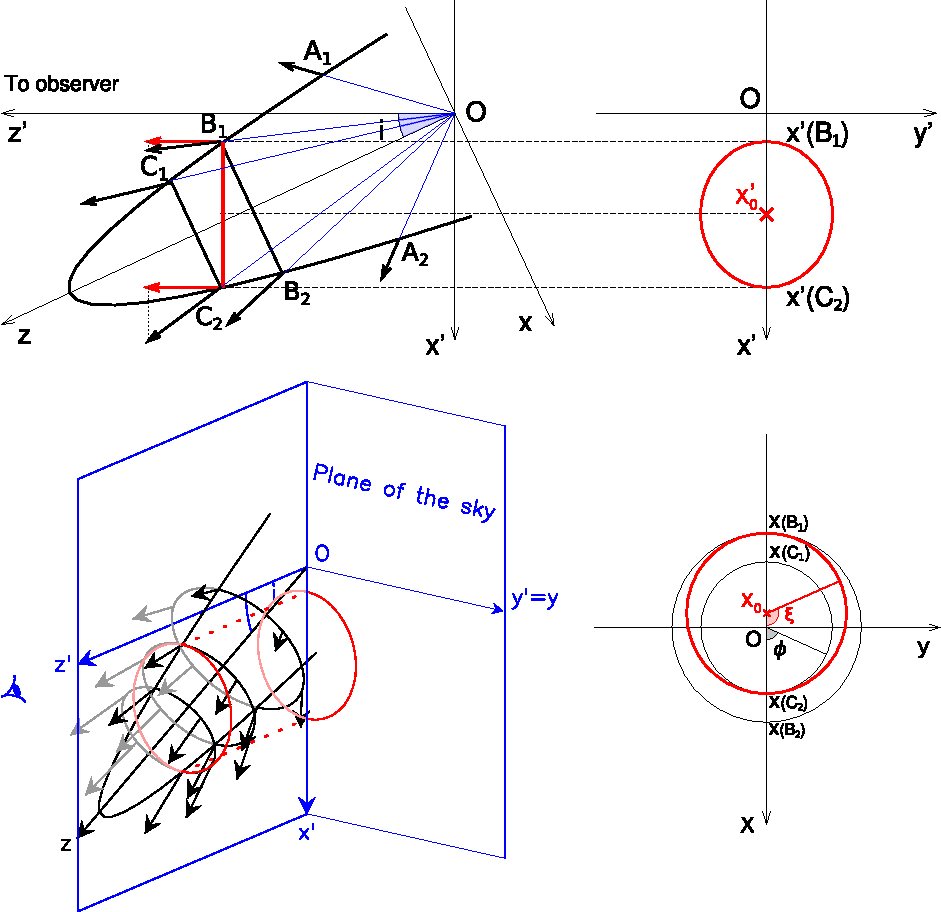
\includegraphics[width=\textwidth]{figures/geometry_ballistic.pdf}\\
 \label{fig:scheme}
\end{figure*}
\begin{figure}[p!]
{\bf Extended Data Fig.\ 3: Geometry of the ballistic model.} Geometrical scheme of a shell of ejected material and of the reference coordinate systems. The Cartesian coordinate system associated with the shell is $(x,y,z)$, where $z$ is its symmetry axis. The coordinate system of the observer is $(x',y',z')$, where the $z'$-axis is the LOS, oriented at an inclination angle $i$ from the $z$-axis, and the axes $y$ and $y'$ are coincident. The $x'y'$-plane is the plane of the sky. The origin of coordinates for both systems is the position of the star. Thus, the two coordinate systems are related by a rotation of angle $i$ around the $y$(=$y'$)-axis. 
{\bf Top left:} Side view, where the coplanar axes $x$, $x'$, $z$, and $z'$-axes are contained in the plane of the page, while the $y$(=$y'$)-axis is perpendicular to it, coming out of the page. Because of the axial symmetry, the points with the same $z$ have the same speed, which increases with $z$. The velocity vectors are represented by black arrows, where the pairs of points A$_1$-A$_2$, B$_1$-B$_2$, and C$_1$-C$_2$ have the same speed (proportional to the arrow length). The plot illustrates the case of a paraboloidal shell. Due to projection and velocity gradient effects, points with different speeds can have the same LOS velocity component (e.g., points B$_1$ and C$_2$, whose LOS velocity components are shown as red arrows). The set of points of the shell with a given LOS velocity component define an iso-LOS velocity curve (the one containing points B$_1$ and C$_2$ is shown in red). In the case of a paraboloidal shell formed by material ejected radially and simultaneously, the iso-LOS velocity curves are ellipses parallel to the plane of the sky (see Methods).
 {\bf Top right:} Projection (shown in red) of the iso-LOS velocity curve onto the plane of the sky ($x'y'$-plane). The projections of points B$_1$ and C$_2$ are labeled as $x'$(B$_1$) and $x'$(B$_2$). The point $x'_0$ is the center of the observed ring and corresponds to the projection of the center of the iso-LOS curve. In this plot, both the iso-LOS curve and its projection are ellipses. Note that the center of the iso-LOS curve does not fall on the symmetry axis of the shell (the $z$-axis) but slightly above it.
 %, so $x'_0$ does not correspond 
 %, which is an ellipse in the figure. Note that the symmetry axis of the shell 
 %Note that this point does not correspond to the projection of the intersection of the symmetry axis of the shell (the $z$-axis) with the plane containing the iso-LOS velocity curve.???
 {\bf Bottom left:} Three-dimensional scheme of the ejected shell. The intersection of the shell with the $x'z'$ plane is shown as a black curve. Several cross-sections of the shell and their velocity vectors are plotted as black/gray ellipses and arrows, according to the positions of the points relative to the $x'z'$-plane (black for points with $y'$$>$0 and gray for $y'$$<$0). An iso-LOS velocity curve and its projection onto the plane of the sky are shown in red.  
 {\bf Bottom right:} Projection of transverse sections of the shell onto the $xy$-plane, at two different heights (black circles), corresponding to the points B$_1$, B$_2$ and C$_1$, C$_2$ defined in the top left panel. The red curve is the projection onto the $xy$-plane of the iso-LOS velocity curve (a circle in the case of the aforementioned paraboloidal model, with center at ($x_0,0$); see Methods). The angle $\phi$ is the azimuthal angle in the shell coordinate system, with its origin in the star, while $\xi$ is the angle measured from $x$, also contained in the $xy$-plane, but centered on $x_0$.
\end{figure}



A simple, purely geometrical model was developed to interpret the shape, size, and position of the rings observed in the velocity channel maps of the shells ejected by the young stellar object SVS~13.
The model assumes two hypothesis: 
i) all the material in a given shell is ejected from the star (or from very near to it) at the same time, and moves ballistically in a purely radial direction,
with a constant velocity equal to the velocity of ejection; and ii) the shape of the shell can be approximated by a paraboloid of revolution, symmetric about the flow axis.

\subsection{Model parameters}

We are considering the shell reference frame, with its origin at the position of the YSO, the $z$ axis along the shell axis, the $y$ axis perpendicular to $z$ and on the plane of the sky, and the $x$ axis perpendicular to both $z$ and $y$. The shell axis has an inclination $i$ with respect to the LOS. The observer reference frame has the same origin, with the $z'$ axis along the LOS, toward the observer, the $x'$ axis along the projection of the shell axis on the plane of the sky, and the $y'$ axis coinciding with the $y$ axis, so that the plane $x'y'$ is the plane of the sky (see Extended Data Fig.~3). Thus, the two coordinate systems are related by a rotation of angle $i$ around the $y$(=$y'$)-axis, and the transformation between the two sets of coordinates is
\begin{equation}\label{eq:coord}
\left\{\begin{array}{rcl}
x' &=& x \cos i + z \sin i, \\
y' &=& y, \\
z' &=& z \cos i - x \sin i.
\end{array}\right.
\end{equation}
The equation of the paraboloid can be written as
\begin{equation}\label{eq:parabola}
x^2+y^2= a^2 z_\mathrm{apex} (z_\mathrm{apex}-z),
\end{equation}
for $0\le z \le z_\mathrm{apex}$, where $z_\mathrm{apex}$ is the location of the apex of the paraboloid, and $a$ is a dimensionless parameter such that the radius of the paraboloid at $z=0$ is $a\, z_\mathrm{apex}$. %$a$ times $z_\mathrm{apex}$. 
The degree of collimation of the ejection increases with decreasing values of $a$.
The shape of the shell depends on two parameters, the distance of the paraboloid apex from the YSO, $z_\mathrm{apex}$, and the collimation parameter, $a$.
A third parameter of the model is the time elapsed from the ejection, or dynamical time of the shell, $t_\mathrm{dyn}$, which gives the relationship between velocities and distances from the YSO.
In particular, the maximum ejection velocity, along the axis of the shell, $v_\mathrm{apex}$, is given by
\begin{equation}
	v_\mathrm{apex}= \frac{z_\mathrm{apex}}{t_\mathrm{dyn}}.
\end{equation}

\subsection{Channel maps}

The velocity of a channel map, $v_\mathrm{ch}$, is the LOS velocity relative to the YSO as measured by the observer, and is defined positive when the motion is away from the observer (redshifted). However, the system of coordinates used has the $z'$ axis directed toward the observer and, thus, positive $v_{z'}$ velocities are directed toward the observer (blueshited). Therefore, there is a change of sign between $v_\mathrm{ch}$ and $v_{z'}$:
 %The system of coordinates used has the $z'$ axis directed toward the observer. Thus, a velocity toward the observer (blueshifted) is defined positive, while the velocity of a channel map, $v_\mathrm{ch}$, is the LOS velocity relative to the YSO as measured by the observer, and has the opposite sign. Therefore 
%%Thus, positive $v_{z'}$ velocities are blueshifted, that is, negative LOS velocities with respect to the YSO measured by the observer, $v_\mathrm{ch}$, so that
% {\bf
% 	We define $v_\mathrm{ch}$ as the velocity associated to a channel map (relative to the systemic velocity, where $v_\mathrm{ch}>0$ if redshifted and $v_\mathrm{ch}<0$ if blueshifted). All points of a ring observed in a channel map with velocity $v_\mathrm{ch}$ correspond to points that belong to a LOS isovelocity curve with $v_{z'}(z,\phi)$=-$v_\mathrm{ch}$. Equation (14) becomes:
% }
\begin{equation}
v_\mathrm{ch}= -v_{z'}= -\frac{z'}{t_\mathrm{dyn}}.
\end{equation}

The observed image of the emission of the shell in a spectral channel with LOS velocity $v_\mathrm{ch}= -v_{z'}$ will be an elliptical ring, corresponding to the projection onto the plane of the sky of the intersection of the shell with the iso-LOS velocity plane $z'= -v_\mathrm{ch}\,t_\mathrm{dyn}$. Since the iso-LOS velocity plane is parallel to the plane of the sky, the ellipse remains unchanged in this projection. 
 %The image (in a channel map???) of the emission of the shell at a given LOS velocity $v_\mathrm{ch}= -v_{z'}$ will be an elliptical ring, corresponding to the intersection of the shell with the iso-LOS velocity plane $z'= -v_\mathrm{ch}\,t_\mathrm{kin}$, which is parallel to the plane of the sky. 
The size of the elliptical rings decreases with increasing $v_{z'}$, and becomes zero for $v_{\rm tip}$, the maximum value of $v_{z'}$, near (but not coinciding with) the apex of the shell.
The centroid of the rings is located along the $x'$ axis, at a distance $x_0'$ from the origin, increasing with increasing $v_{z'}$ (see Extended Data Fig.~3).
In the following we will derive the shape, size, and position of these elliptical rings.

By using equation (\ref{eq:coord}), the iso-LOS velocity plane $z'= -v_\mathrm{ch}\,t_\mathrm{dyn}$ transforms in
\begin{equation}
z= x \tan i -\frac{v_\mathrm{ch}\,t_\mathrm{dyn}}{\cos i}.\label{eq:z}
\end{equation}
By substitution in the paraboloid equation, we obtain
\begin{equation}
(x-x_0)^2+y^2= r_c^2, \label{eq:xycirc}
\end{equation}
%{\color{red} which is the equation of a circumference of center $(x_0,0)$ and radius $r_e$ in the shell reference frame},
with
\begin{eqnarray}
	x_0 &=& -\frac{a^2 z_\mathrm{apex}}{2}\tan i, \label{eq:x0}\\
	r_c^2 &=& a^2 z_\mathrm{apex}\left[\frac{v_\mathrm{ch}\,t_\mathrm{dyn}}{\cos i}+z_\mathrm{apex}\left(1+\frac{a^2}{4}\tan^2 i\right)\right].\label{eq:r}
\end{eqnarray}
Equations (\ref{eq:z}) and (\ref{eq:xycirc}) are the equations of the iso-LOS velocity curve in the shell reference frame. Note that equation (\ref{eq:xycirc}), which gives the projection onto the $xy$ plane of this curve, is a circumference of center ($x_0$, 0) and radius $r_c$.
The parametric equations of the 3D coordinates of the intersection of the paraboloid and the iso-LOS plane can be obtained by using $x=x_0+r_c\cos\xi$, $y=r_c\sin\xi$ (where $0\le \xi< 2\pi$ is the polar angle in the $xy$ plane with respect to the $x$-axis), and equation~(\ref{eq:parabola}), resulting:  
\begin{equation}\label{eq:xyproj}
\left\{\begin{array}{r@{\ }c@{\ }l}
x &=& x_0+r_c\cos \xi, \\
y &=&     r_c\sin \xi, \\
%z &=& z_\mathrm{ap}-\displaystyle\frac{x_0^2+r^2}{a^2 z_\mathrm{ap}}-\frac{2 x_0}{a^2 z_\mathrm{ap}} r \cos \varphi,
z &=& z_\mathrm{apex} -\displaystyle\frac{x^2+y^2}{a^2 z_\mathrm{apex}}=
z_\mathrm{apex}-\displaystyle\frac{x_0^2+r_c^2}{a^2 z_\mathrm{apex}}+r_c\tan i \cos \xi.
\end{array}\right.
\end{equation}

By using equation (\ref{eq:coord}), the above equations can be transformed to the observer reference frame, obtaining their projection on the plane of the sky:
\begin{equation}\label{eq:ring}
\left\{\begin{array}{r@{\ }c@{\ }l}
x' &=& x'_0+f r_c\cos\xi,\\
y' &=& r_c\sin \xi,       
\end{array}\right.
\end{equation}
where $r_c$ is given by equation (\ref{eq:r}) and
\begin{eqnarray}\label{eq:x'0}
	x'_0 &=& -v_\mathrm{ch}\,t_\mathrm{dyn} \tan i-\frac{a^2 z_\mathrm{apex}}{2}\frac{\tan i}{\cos i}, \\
	f &=& \frac{1}{\cos i}>1.
\end{eqnarray}
Equations (\ref{eq:ring}) are the parametric equations of an ellipse centered on $(x'_0, 0)$, with
a semi-axis in the $x'$ direction $f r_c$,
a semi-axis in the $y'$ direction $r_c$,
and a longitudinal to transverse axial ratio $f=1/\cos i$, which is a measure of the elongation factor of the ellipse.
 %, or flattening, $f=1/\cos i$.
Since $f>1$, the ellipse is elongated along the $x'$ direction.

The maximum absolute value of the LOS velocity occurs at the tip of the shell, the point closest to the observer, near the apex. 
At this position the ring has zero size, $r_c= 0$, with a channel velocity 
\begin{equation}\label{eq:z0}
	v_\mathrm{tip}= -\frac{z_\mathrm{apex}\,\cos i}{t_\mathrm{dyn}}\left(1+\frac{a^2}{4}\tan^2 i\right).
\end{equation}
In terms of $v_\mathrm{tip}$, the semi-minor axis of the elliptical ring can be given as
\begin{equation}\label{eq:ry'}
	r_c^2= a^2 z_\mathrm{apex}\left(\frac{v_\mathrm{ch}-v_\mathrm{tip}}{\cos i}\,t_\mathrm{dyn}\right).
\end{equation}


\subsection{Derivation of shell parameters from the observation}

Let us assume that we measure, for several channel maps at different velocities $v_\mathrm{ch}$,
the position of the center of the rings, $x'_0$, 
and their semi-minor axis, $r_c$.
As can be seen from equations (\ref{eq:x'0}) and (\ref{eq:ry'}), there are linear relationships of $x'_0$ and $r_c^2$ with $v_\mathrm{ch}$,
\begin{eqnarray}     %\label{eq:xv}
	x'_0  &=& p_x\, v_\mathrm{ch}+q_x,\label{eq:x0'_2} \\
r_c^2 &=& p_r\, v_\mathrm{ch}+q_r,\label{eq:re2_2}
\end{eqnarray}
where the coefficients are
\begin{eqnarray}
p_x &=& -t_\mathrm{dyn} \tan i,\label{eq:px_2} \\
q_x &=& -b\,\frac{\tan i}{2\cos i},\label{eq:qx_2} \\
p_r &=& \phantom{-} b\,\frac{t_\mathrm{dyn}}{\cos i},\label{eq:pr_2}\\
q_r &=& -b\,\frac{t_\mathrm{dyn}}{\cos i}v_\mathrm{tip},
\end{eqnarray}
and, for simplicity, we used $b\equiv a^2\,z_\mathrm{apex}$.
For a given inclination, there are four parameters ($p_x$, $p_r$, $q_x$, and $q_r$), but the independent parameters that define the shape and kinematics of the shell are three, $t_\mathrm{dyn}$, $v_\mathrm{tip}$, and $b$ (equivalent to $t_{\rm dyn}$, $z_\mathrm{apex}$, and $a$).

A simple way of fitting the three independent parameters is to note that the independent term $q_x$ is much smaller than the others.
Its physical interpretation is the position of the center of the rings extrapolated to $v_\mathrm{ch}=0$, and should be near zero.
Thus, an iterative procedure, can be performed, beginning with $q_x=0$.
At each step, the fits $x'_0-q_x= p_x\, v_\mathrm{ch}$ (with $q_x$ fixed) and $r_c^2= p_r\, v_\mathrm{ch}+q_r$ (equations (\ref{eq:x0'_2}) and (\ref{eq:re2_2})) are calculated, 
and $q_x$ is recalculated (using equations (\ref{eq:px_2})-(\ref{eq:pr_2})) as $q_x= (p_r/2p_x)\tan^2 i$.
The process converges easily to values of $p_x$, $p_r$, and $q_r$ consistent with $q_x$.
Once the best fit values of $p_x$, $p_r$, and $q_r$ are obtained, the shell parameters are derived (equations (\ref{eq:x'0}) and (\ref{eq:ry'})) as
\begin{eqnarray}
t_\mathrm{dyn} &=& -\frac{p_x}{\tan i}, \\
v_\mathrm{tip} &=& -\frac{q_r}{p_r}, \\
b          &=& -\frac{p_r}{p_x}\,\sin i.
\end{eqnarray}
The rest of parameters of the shell are derived (equation (\ref{eq:z0})) as
\begin{eqnarray}
	z_\mathrm{apex} &=& -\frac{v_\mathrm{tip} t_\mathrm{dyn}}{\cos i} -\frac{b}{4} \tan^2 i= 
-\frac{p_x q_r}{p_r \sin i} +\frac{p_r}{4 p_x} \sin i \tan^2 i, \\
a   &=& \sqrt{\frac{b}{z_\mathrm{apex}}}, \\
v_\mathrm{apex} &=& \frac{z_\mathrm{apex}}{t_\mathrm{dyn}}. 
\end{eqnarray}



\begin{figure}[p!]
\begin{center}
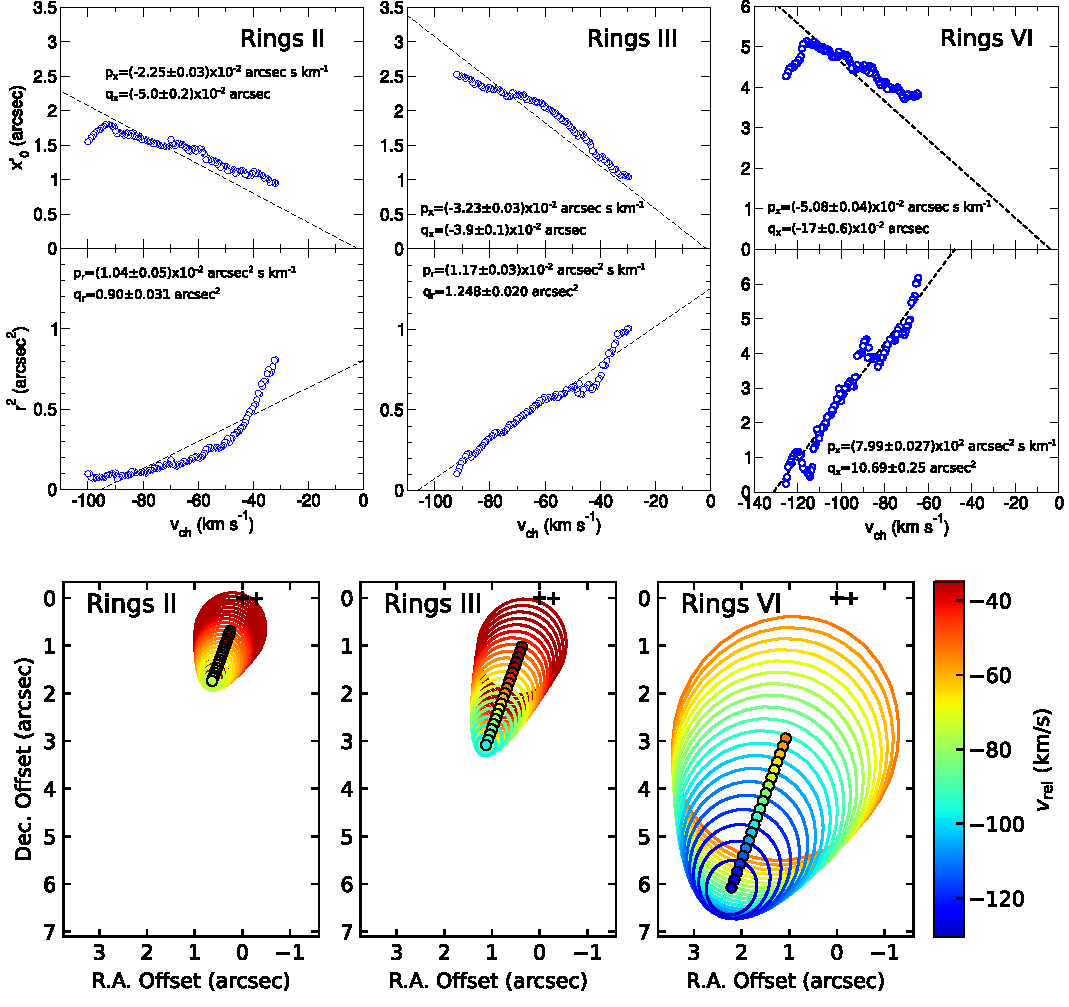
\includegraphics[width=\textwidth]{figures/paraboloid_fits.pdf} 
\caption[Results of the paraboloidal shell model fitting.]{{\bf Results of the paraboloidal shell model fitting.} Plots of the results of the fitting of a geometrical model consisting of a paraboloidal shell of material ejected simultaneously from the source, moving radially at constant velocitiy (see Methods). An inclination angle $i$ = 25$^\circ$ is adopted (see Methods). {\bf Top:} Position of the center, $x'_0$, and radius squared, $r^2$, of the rings as a function of the velocity relative to the source of the channel map, $v_\mathrm{ch}$, for families of rings II, III, and VI. {\bf Bottom:} Projection of the (elliptical) iso-LOS velocity curves onto the plane of the sky, for different color-coded LOS velocities (relative to the source), corresponding to the best-fit model parameters.
 %for families of rings II, III, and VI.
 We obtain deprojected velocities at the apex $v_\mathrm{apex}$ = 95.3$\pm$5.8, 116.9$\pm$4.0, 146.3$\pm$6.2~\kms; dynamical times $t_\mathrm{dyn}$ = 68.5$\pm$0.8, 98.4$\pm$0.8, and 155.2$\pm$1.1~yr; and values of the parameter that controls the degree of collimation (see equation (\ref{eq:parabola})) $a$ = 0.206$\pm$0.008, 0.138$\pm$0.003, and 0.204$\pm$0.006, for families of rings II, III, and VI, respectively.}
\label{fig:parafit}
\end{center}
\end{figure}


\subsection{Application to SVS~13}

Top panels of Extended Data Fig.~4 show the plots of the positions of the center of the rings, $x'_0$, and square of radii, $r_c^2$, versus the LOS velocity relative to the source, $v_\mathrm{ch}$, for the families of Rings II, III, and VI.
The rings are almost circular, implying that the inclination is small.
For the inclination angle adopted, $i= 25^\circ$, the axial ratio expected is $f=1/\cos{i}=1.10$, compatible with the values measured for the rings. 
%of major to minor axes measured for the rings.
It is remarkable that, in general, the position of the rings and the square of their radii depend roughly linearly on the channel velocity, as predicted by the model.
The plot also shows the consistent linear fits to the data, which fit pretty well the observations.
The fit parameters obtained ($p_x$, $p_r$, $q_x$, and $q_r$) are shown in the top panels of Extended Data Fig.~4. 
%The values in practical units are calculated for a distance of 300 pc.
The parameters of the paraboloid shell for each family have been obtained from the fit parameters in the way explained above, and are listed in the caption of Extended Data Fig.~4. We obtain deprojected velocities at the apex, $v_\mathrm{apex}$ = 95.3$\pm$5.8, 116.9$\pm$4.0, and 146.3$\pm$6.2 \kms, and dynamical times of the shell, $t_\mathrm{dyn}$ = 68.5$\pm$0.8, 98.4$\pm$0.8, and 155.2$\pm$1.1 yr, for Rings II, III, and VI, respectively.



\section{Ballistic deprojection}

%\subsection{\bf Analytical deprojection of {\color{blue} of rings created by a radially expanding, ballistic shell of arbitrary axisymmetric shape}\label{sec:deprojection}

%\subsection{\bf Deprojection of rings created by a radially expanding, ballistic shell of arbitrary axisymmetric shape}\label{sec:deprojection}

% \subsection*{\bf Generalized??? ballistic model and deprojection}

% \emph{OJO: Cada vez que se referencie la seccion de Robert, poner as mentioned in the previous section, o ``Name of the Robert's section'' section}

% Poner ``Name'' in Methods

%Here we describe a procedure to obtain the 3D morphology and kinematics of an axisymmetric shell of arbitrary shape using the sizes, positions and LOS velocities of the corresponding family of rings. 

%Here we describe a procedure to obtain the 3D morphology and kinematics of an arbitrarily shaped axisymmetric shell using the sizes, positions and LOS velocities of the corresponding ring family. 

Here we describe a procedure to obtain the 3D morphology and kinematics of an arbitrarily shaped axisymmetric ballistic shell from the observed sizes, positions and LOS velocities of the respective ring family. 

%Here we describe a procedure to obtain the 3D morphology and kinematics (shape and velocities) of an axisymmetric shell of arbitrary shape, resulting from the ballistic ejection of material (i.e., expanding radially from the origin with constant velocity),  traced by a given family of rings.

%Here we describe a procedure to obtain the 3D shape and velocities of a ballistic {\color{blue} and radially expanding axisymmetric} shell traced by a given family of rings. A ring observed in a channel map of LOS velocity $v_{\rm ch}$ is the projection of the corresponding iso-LOS velocity curve onto the plane of the sky. Our aim is to infer the deprojected shell morphology and kinematics using measurements of the sizes, positions and LOS velocities of the observed rings. 

Let us consider a one-sided, relatively collimated, ejection of particles distributed in a thin shell observed at an inclination angle $i$ (see Extended Data Fig.~3). We assume that the shell of ejected material is axisymmetric, but with an arbitrary smooth shape. We further assume that all the material has been ejected radially from the proximity of the protostar, over a range of time and velocity, and that each particle moves ballistically with a constant velocity. Therefore, the position and velocity vectors of each particle in the shell are proportional, where the proportionality factor is the time elapsed since its ejection, $t_\mathrm{dyn}$. We adopt the same shell and observer reference frames than in the ``Paraboloid-shell model'' section (see Extended Data Fig.~3), so the transformation between the two frames is given by equations (\ref{eq:coord}), where $x'y'$ is the plane of the sky, the $z'$ axis is along the LOS, and $z$ along 
 %$i$ is the inclination angle of
 the shell axis.

Because the shell is geometrically thin and with axial symmetry, all the points with a given value of $z$ are located at the same distance, $r$, from the $z$-axis. Other geometrical and kinematical properties of the shell can also be written as a function only of $z$. Therefore, for the deprojection, it is convenient to relate the Cartesian coordinates ($x',y',z'$) of the points of the shell in the observer reference frame and their Cylindrical coordinates ($r,\phi,z$) in the shell reference frame, where $\phi = \arctan\left(y/x\right)$ is the azimuthal angle with origin in the $x$-axis. From equations (\ref{eq:coord}), and taking into account that $x=r\cos\phi$ and $y=r\sin\phi$, 
we obtain:
\begin{eqnarray}
\label{eq:xpcoord}
x' &=& x\cos{i} + z\sin{i} = r\cos{\phi}\cos{i} + z\sin{i},\\
\label{eq:ypcoord}
y' &=& y = r\sin{\phi},\\
z' &=& z\cos i - x\sin i= z\cos i - r\cos\phi\sin i.
\end{eqnarray}
% and the channel map velocity
% \begin{equation}
% v_\mathrm{ch} = -v_{z'} = v\left(\sin{\theta}\cos{\phi}\sin{i} -\cos{\theta}\cos{i}\right).
% \end{equation}
Note that, in practice, the only directly measurable lengths are the coordinates $x'$ and $y'$, in the plane of the sky, but not $z'$, along the LOS.

We can also use equations (\ref{eq:coord}) to relate the Cartesian components of the velocity in the reference frames of the observer and the shell. Furthermore, given that the velocity and the position vector for any point of the shell have the same direction (and, therefore, they transform in the same way), we can write:
\begin{eqnarray}
	v_{x'} &=& v_x\cos i + v_z\sin i = v\sin\theta\cos\phi\cos i + v\cos\theta\sin i,\\
	v_{y'} &=& v_{y} = v\sin\theta\sin\phi,\\
\label{eq:vzpcoord}
	v_{z'} &=& v_z\cos i - v_x\sin i = v\cos\theta\cos i - v\sin\theta\cos\phi\sin i, 
\end{eqnarray}
where $v$ is the speed, and $\theta=\arctan\left(r/z\right)$ and $\phi$ (defined above) are the polar and azimuthal angles, respectively, of the position vector in the shell reference frame (see Extended Data Fig.~3). Note that the only measurable velocity in our spectral line observations is $v_{z'}$, the velocity projected onto the LOS $z'$ (i.e, $v_{z'}$=$-v_{\rm ch}$, where $v_{\rm ch}$ is the velocity of the channel map). Nevertheless, a second epoch of observation could potentially provide measurements of $v_{x'}$ and $v_{y'}$ through proper motions in the plane of the sky.

%Note that the only measurable velocity in our spectral line observations is the velocity projected onto the LOS $z'$, $v_{z'}=-v_{\rm ch}$, where $v_{\rm ch}$ is the central velocity of the channel map. 

Therefore, equations (\ref{eq:xpcoord}), (\ref{eq:ypcoord}), and (\ref{eq:vzpcoord}) relate the measurable parameters in the channel maps and the parameters of the shell. For a given value of $z$, these equations are simplified when $\phi=\pi/2$ (the same result is obtained taken $\phi=3\pi/2$, because of symmetry), resulting:
\begin{eqnarray}
\label{eq:zdprj}
z &=& \frac{x'_{\pi/2}}{\sin{i}},\\
\label{eq:Rdprj}
r &=& y'_{\pi/2},\\
\label{eq:vdprj}
v &=& \frac{v_{z'}\,\sqrt{r^2+z^2}}{z\cos i},
%%v &=& - v_\mathrm{ch}\,\sqrt{R^2+z^2}/\left(z\cos{i}\right),
%v_\mathrm{ch} &=& -v_{z'} \simeq -v \cos{\theta}\cos{i},
\end{eqnarray}
where $x'_{\pi/2}$ and $y'_{\pi/2}$ are the Cartesian coordinates in the observer reference frame of the point of the shell with $\phi=\pi/2$ and projected velocity $v_{z'}$.

%LOS velocity $v_{z'}=-v_{\rm ch}$, where $v_{\rm ch}$ is the central velocity of the channel map.

 %and projected velocity $v_{z'}$.
 %vch=-vz' is the central velocity of the channel map considered.
 For a given value of $z$, the point $(x'_{\pi/2}, y'_{\pi/2})$ is the one with the largest value of $y'$, which coincides with the radius, $r$, of the cross-section of the shell at $z$, as this transverse distance remains unaffected by the projections. However, it should be noted that an observed channel map is the image of the points of the shell that have the same projected LOS velocity $v_{z'}=-v_{\rm ch}$, where $v_{\rm ch}$ is the central velocity of the channel map, and these points correspond to a range of values of $v$ and $z$ in the 3D shell. Since the radius of the shell changes with $z$ (in general, increases as $z$ decreases), the point in a channel map with the largest value of $y'$, in general does not correspond exactly to $\phi=\pi/2$ and $z=x'_{\pi/2} / \sin{i}$. 

%Because we are assuming that the shell of ejected particles is a surface of revolution around the $z$-axis, the projection onto the plane of the sky of the LOS isovelocity curves will be symmetric with respect to the $x'$-axis (the projection of the $z$-axis onto the plane of the sky). In general, these projected curves, as observed in the velocity channel maps, can be approximated as elliptical rings, with their centers, and either their major or minor axis, located on the $x'$-axis. The $x'$-coordinate of the center of the observed rings, $x_{\rm center}'$ (which can be obtained by fitting ellipses to the observed channel map images), is taken as the $x'$-coordinate of the center of the corresponding (true) ring in the shell, which is given by $x'(z, 90^\circ)$. This is a good approximation provided the shape of the observed rings is roughly symmetric with respect to an axis perpendicular to the $x'$-axis and intersecting it at $x_{\rm center}'$ or, equivalently, if in the three-dimensional space the centers of the LOS isovelocity curves approximately fall on the $z$-axis. Then, using equations (3) and (16), we can write:

 Therefore, in general, the observations only provide approximate coordinates of the point with $\phi=\pi/2$, and equations (\ref{eq:zdprj}) and (\ref{eq:Rdprj}) are only used approximately. In general, the agreement will be better the smaller the variation of the shell radius with $z$, i.e., it would be a good approximation for a well-collimated shell. For the paraboloid-shell with a single ejection time discussed before (see `Paraboloid-shell model' section) the curves of equal LOS velocity are ellipses contained in planes parallel to the plane of the sky. However, the centers of these ellipses do not fall exactly onto the $z$ axis (see Extended data Fig.~3) but, at a position $(x'_0, 0)$ with $x'_0 < z \sin i$. For the paraboloidal shell case, $x'_0$ can be calculated (equation (\ref{eq:x'0})) and it can be shown that the shift is $\ll r/2$, except for points very close to the apex ($z_{\rm apex}-z\la r$). In the general case discussed here, the shell is axisymmetric but the ejection of the whole shell does not necessarily occur simultaneously, thus the iso-LOS velocity curves are not necessarily contained in planes perpendicular to the LOS axis $z'$, and the projections of the iso-LOS velocity curves onto the $x'y'$-plane (the plane of the sky) are symmetric with respect to the $x'$-axis, but not necessarily elliptical. Nevertheless, our observations show that the observed rings in the channel maps can be fitted pretty well as ellipses, and we use the fitted positions of the centers of the ellipses, $x'_0$, their transverse semi axes, $r_{y'}$, and the velocity of the observed channel maps, $-v_{\rm ch}$, as our estimates for $x'_{\pi/2}$, $y'_{\pi/2}$, and $v_{z'}$ in equations (\ref{eq:zdprj}), (\ref{eq:Rdprj}), and (\ref{eq:vdprj}). We expect the degree of accuracy to be similar to the paraboloid case, and therefore that the deprojection is accurate, except very close to the head of the shell. Therefore, by fitting ellipses to the observed rings in the channel maps the deprojected structure of the shell, $r(z)$ and $v(z)$, can be obtained and tabulated as a function of $z$. We can also obtain the polar angle of the points in the shell reference system as:
\begin{equation}\label{theta(z)}
\theta(z) = \arctan\left(\frac{r}{z}\right).
\end{equation}
Finally, since the particles are assumed to move in straight lines and with constant velocity, we can obtain the dynamical time as: 
\begin{equation}\label{eq:tkin}
	t_\mathrm{dyn}(z)=\frac{\sqrt{r^2+z^2}}{v},
\end{equation}
where $r(z)$ and $v(z)$, can be taken from the tabulated values that are obtained using equations (\ref{eq:Rdprj}) and (\ref{eq:vdprj}). Since all points with a given value of $z$ have the same values of $r$ and $v$, all will also have the same dynamical time.
%{\color{red} Thus, by measuring $x'_0$??? and $r_{y'}$??? (center and transverse axis of the ellipses fitted to the rings???) of the rings of a given family in every channel map with velocity $v_\mathrm{ch}$, we would obtain how $R$ and $v$ vary with $z$, and thus, the approximate deprojected shape and kinematics of the shell.???
%}

% Thus, 
% \begin{eqnarray}
% \label{eq:zdprj}
% z &\simeq& x'_0 / \sin{i},\\
% \label{eq:Rdprj}
%  R &\simeq& r_{y'},\\
% \label{eq:vdprj}
% v &\simeq& - v_\mathrm{ch}\,\sqrt{R^2+z^2}/\left(z\cos{i}\right).
% %v_\mathrm{ch} &=& -v_{z'} \simeq -v \cos{\theta}\cos{i},
% \end{eqnarray}
%By measuring $x'_0$ and $r_{y'}$ of the rings of a family in every channel map with velocity $v_\mathrm{ch}$, we would obtain how $R$ and $v$ vary with $z$, and thus, an approximated deprojected shape and kinematics of the shell.


In order to relate the derived properties of the ejected shell with the observed emission, additionally to the global shell structure, we will derive the $z$-coordinate corresponding to every pixel of the observed rings. In this way, we will be able to relate the intensity of the observed CO(3-2) emission in the channel maps with the 3D kinematical and geometrical properties (e.g., $v(z)$, $r(z)$, $t_{\rm dyn}(z)$) of the location in the shell where this emission was originated. From equation (\ref{eq:vzpcoord}), assuming $i\neq0$, the azimuthal angle $\phi$ and $z$ are related by the following equation:
 \begin{equation}\label{eq:cosphi}
 \cos\phi = \frac{1}{\tan\theta\tan i} + \frac{v_\mathrm{ch}}{v\sin\theta\sin i}.
 %\cos\phi(z, v_\mathrm{ch}) = \frac{1}{\tan\theta(z)\tan i} - \frac{v_\mathrm{iso}}{v(z)\sin\theta(z)\sin i}.
\end{equation}
 %assuming $i\neq0$. 
 %In case $i=0$, $\phi$ could take any value given a $z$, being $z$ determined by $v_\mathrm{iso} = v(z)\cos\theta(z)$; but if $i\neq0$, then $\phi$ and $z$ are coupled given a $v_\mathrm{iso}$. 
Substituting equation (\ref{eq:cosphi}) into equation (\ref{eq:xpcoord}), we obtain:
 %a relationship between $x'$ and $z$ for points belonging to a given LOS isovelocity curve with $v_{z'}$=$v_\mathrm{ch}$:
\begin{equation}
x' = r \left(\frac{1}{\tan\theta\tan i}+\frac{v_\mathrm{ch}}{v\sin\theta\sin i} \right)\cos i + z \sin i.
\end{equation}
 %$$x' = \sqrt{R^2+z^2} \left[\sin\theta\left(\frac{1}{\tan\theta\tan i}+\frac{v_\mathrm{ch}}{v\sin\theta\sin i} \right)\cos i + \cos\theta\sin i\right]???. 
And, after some algebra, we get
\begin{equation}
	x'= \frac{z}{\sin i} + \frac{v_\mathrm{ch} \sqrt{r^2+z^2}}{v \tan i},
\end{equation}
or, as a function of the dynamical time,
\begin{equation}\label{eq:xpdprj}
	x'=\frac{z}{\sin i } + t_\mathrm{dyn}\,\frac{v_\mathrm{ch}}{\tan i \,}.
\end{equation}


%%This can also be written as
%%\begin{equation}
%%	x'(z, v_\mathrm{iso})=\frac{z}{\sin i }\left(1 - \frac{v_\mathrm{iso}\cos^2
%%	i}{v_{z'}(z,90^\circ)}\right),
%%\end{equation}
%%or
%%\begin{equation}
%%	x'(z, v_\mathrm{iso})=\frac{x'(z,90^\circ)}{\sin^2 i }\left(1 -
%%	\frac{v_\mathrm{iso}\cos^2 i}{v_{z'}(z,90^\circ)}\right).
%%\end{equation}

Given a value of $x'$ measured in a ring image observed in a channel map with LOS velocity $v_{\rm z'}=-v_{\rm ch}$, we can use the tabulated function $t_{\rm dyn}(z)$ to obtain the values of $z$ and $t_{\rm dyn}$ that satisfies equation (\ref{eq:xpdprj}). Once the value of $z$ is obtained, all the properties of this point of the shell can be obtained from the tabulated values derived from the global deprojection of the shell.

 %As expected, any point of the shell with different $x'$ in a spectral channel map of velocity $v_\mathrm{ch}$ have different projections onto the $z$-axis. Note that, given a spectral channel map with velocity $v_\mathrm{ch}$, in order to determine the dynamical time at any point of the isovelocity curve, we only need to estimate which is its projection onto the $z$-axis. Any of these last four equations allow us to get what $z$ is associated to every $x'$ of the points of the isovelocity curve from a given a spectral channel map; that is, $z(x', v_\mathrm{ch})$.  It is possible to obtain $z(x', v_\mathrm{ch})$ numerically from any of the last four equations, since we have, for example, $t_\mathrm{dyn}(z)$, or $r(z)$ and $v(z)$, from the results of the deprojection. Once we obtain what $z$ is associated to every $x'$ of the isovelocity curve, we can obtain the dynamical time $t_\mathrm{dyn}(z(x',v_\mathrm{ch}))$; that is, the dynamical time of the points with $x'$ that belong to the isovelocity curve with projected velocity $v_\mathrm{ch}$. Thus, if we mask the observed rings with elliptical annulii, and rotate these spectral channel maps considering the position angle of the jet in such a way that origin would be located at the north, the mass associated to a row of pixels will have the same dynamical time, since they have the same $x'$ and consequently the same $z$. 

%We note that this deprojection is valid for a geometrically thin axisymmetric shell, and is useful to deproject the emission which is located near the source, where $\theta (z)$ is significant, so every position vector
%{\boldmath$r$}($z$) 
 %of the shell points forms an angle with the LOS significantly different from $i$ (the inclination angle of the axis of symmetry $z$). For emission far enough from the source or emission that is assumed to lie close to the $z$-axis, so $\theta(z)\simeq 0$, then the deprojection can be performed simply by using the inclination angle $i$ for all the points,

We note that the deprojection procedure described above is valid for a geometrically thin axisymmetric shell, and is useful for deprojecting the emission over most of the shell extent. For points far enough from the source or that lie very close to the $z$-axis (e.g., near the head of the shell), so $\theta(z)\simeq 0$, the deprojection can be performed simply in terms of the inclination angle $i$ (see also the section on dynamical times of the heads in Methods),
\begin{equation}
	v_{\rm head}(z) \simeq -\frac{v_\mathrm{ch}}{\cos i}, 
\end{equation}
and then,
\begin{equation}
	z \simeq \frac{x'_{\rm head}}{\sin i}.
\end{equation}
In this way, the emission near the head, which spreads over filled circles and cannot be treated as geometrically thin rings, can be approximately deprojected using these equations.

\begin{figure}[p!]
\begin{center}
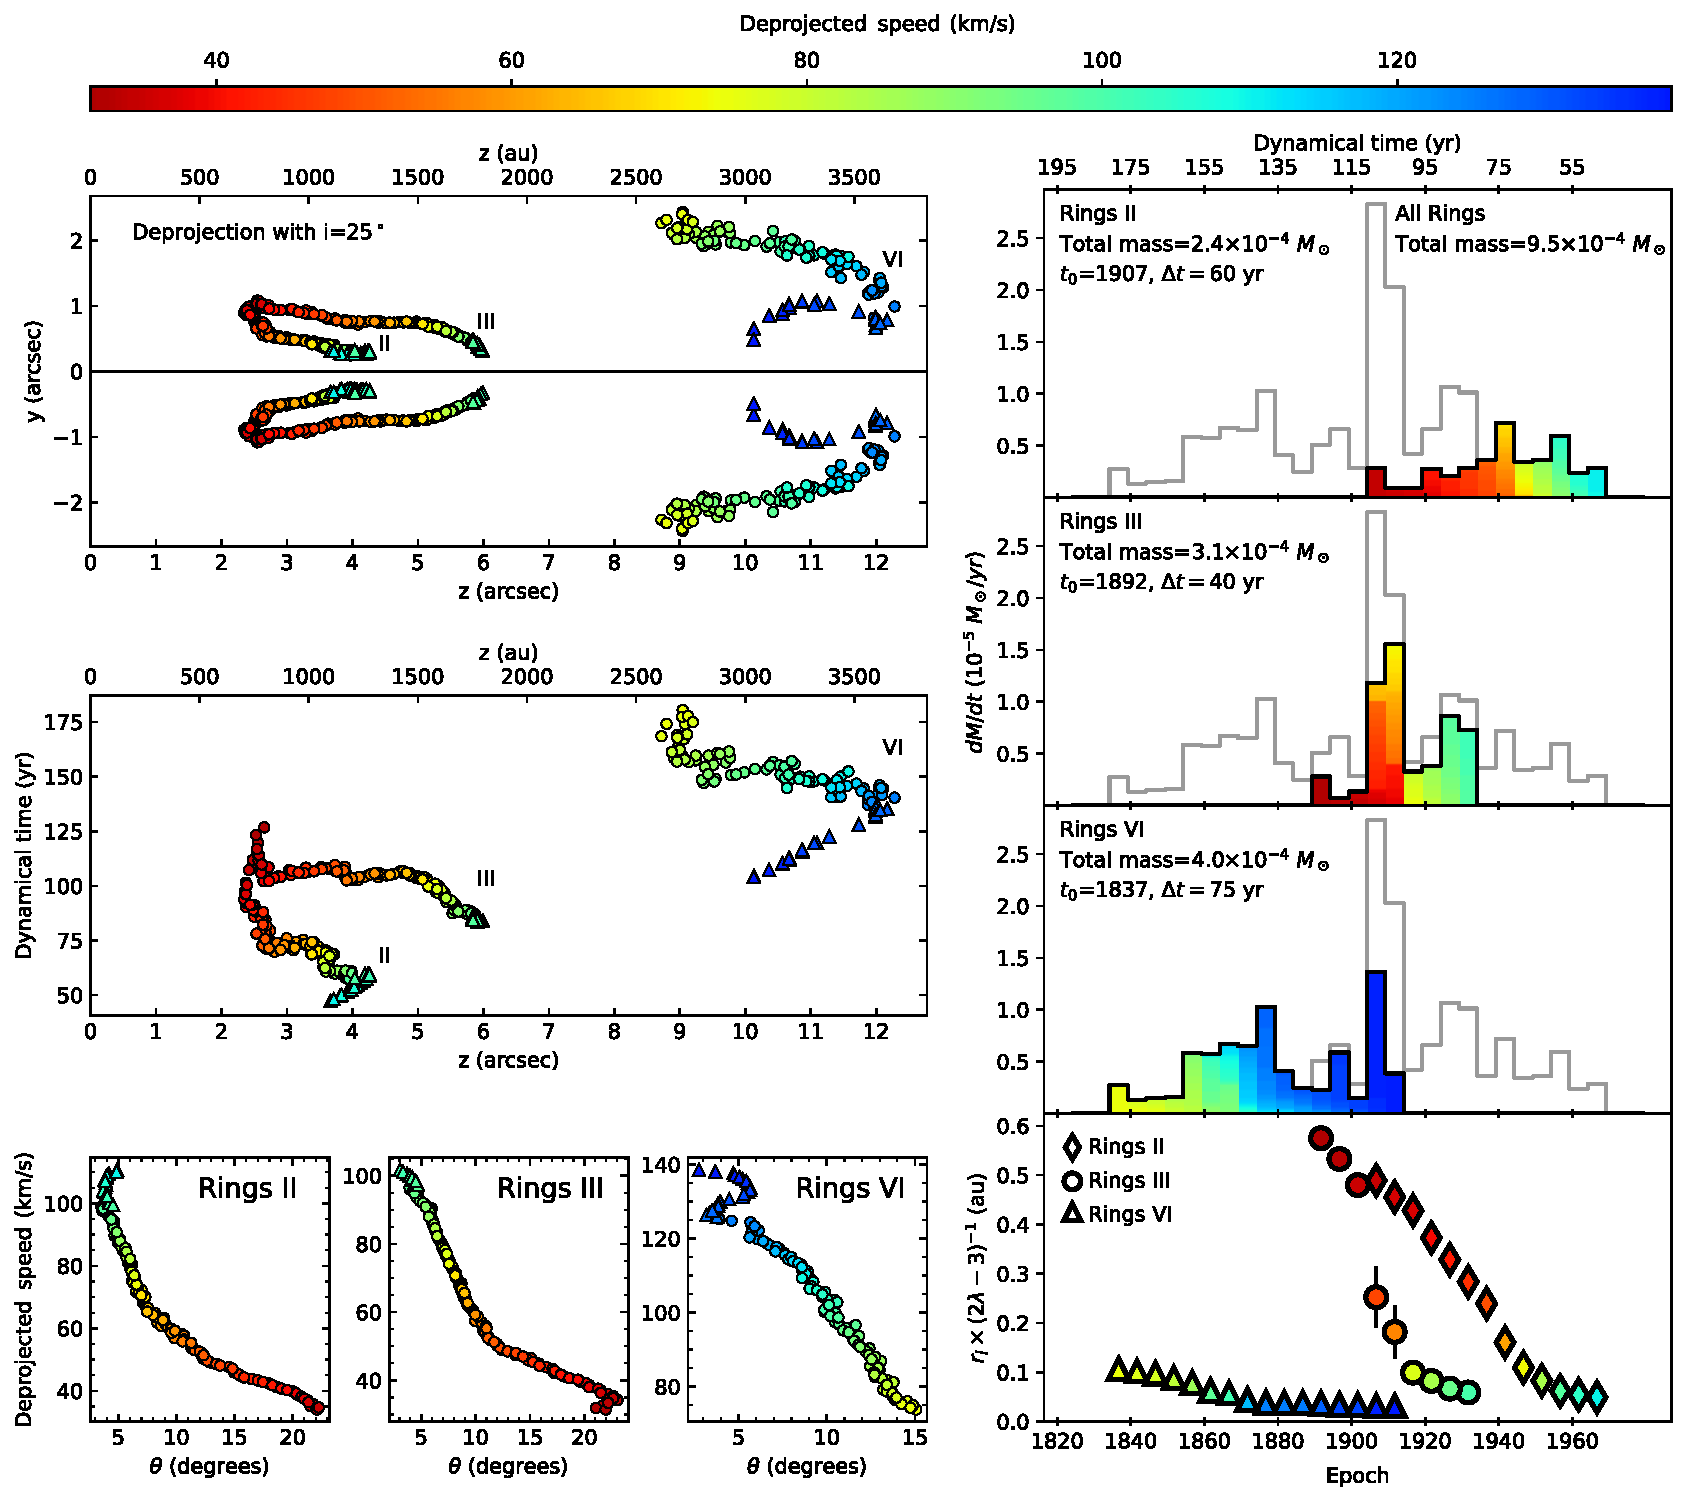
\includegraphics[width=0.91\textwidth]{figures/ballistic_deprojection.pdf}\\
\caption[Results of the ballistic deprojection of the observations]{{\bf Results of the ballistic deprojection of the observations.} Plots resulting from the morphological and kinematical deprojection of the observed families of rings II, III, and VI, assuming an inclination angle $i=25^\circ$ (see Methods). In all panels, the color represents the deprojected velocity. In the left panels color dots indicate the centers of the rings and triangles the regions of filled emission (heads). {\bf Top left panel}: Deprojected morphology of the shells, showing the cylindrical radius, $y$, as a function of distance to the origin along the symmetry axis, $z$. {\bf Middle left panel}: Dynamical time as a function of $z$. {\bf Bottom left panels}: Deprojected velocity as a function of the polar angle $\theta$, defined as the angle of the position vector with respect to the symmetry axis of the shell. {\bf Right panels}: Mass loss history of SVS~13 from epoch 1830 to 1970 in Julian years, with epoch 2000 corresponding to the standard definition of Julian epoch J2000.0. The first three panels (from top to bottom) show the mass-loss rate separated in three ejection events, with a similar pattern of increasing mean speed with time, that are associated with three of the observed families of rings. Data are binned in 5 yr intervals. The color scale indicates the velocity range of the material included in each bin. The bottom right panel shows the estimated launch radius, in the context of a magneto-centrifugal disk wind, as a function of time for every event (see Methods).
}
\label{fig:tkin}
\end{center}
\end{figure}



\subsection{Mass loss rate in the ballistic model.} 

In the framework of the ballistic model (Extended Data Fig.~3) we assume that the observed emission corresponds to material directly ejected from the disk or the close environment of the star. We assume that the ejected material is distributed in a thin shell with axial symmetry around the outflow axis $z$. 
The direction of the velocity is radial from the origin. Therefore, the points with the same magnitude of the velocity, $v$, have the same polar angle, $\theta$, and they are located at the same distance from the origin, $z/\cos\theta$. Thus, they are distributed as circles perpendicular to the outflow direction. These circles would have the same dynamical time. However, these circles of common total velocity do not directly correspond to the elliptical rings observed in images of velocity channels, which correspond to points with the same projected velocity along the LOS ($v_{z'}$). A ring with the same projected velocity is actually composed of points with different total velocities. Above we developed a procedure to deproject the ring images in the observed channel maps.
%Therefore, the points with the same value of $z$ form a thin circular ring. All the points of a given ring are located at the same distance, $r$, from the origin and have the same modulus of the velocity, $v$, and hence the same kinematic time. The direction of the velocity is radial from the origin and therefore all the points in a ring have the same value of the polar angle, $\theta$, with respect to the symmetry axis, with $\theta$ apparently decreasing with $z$. Because of the radial motion and the inclination of the symmetry axis with respect to the LOS, a given ring corresponding to a given value of $z$ will appear split on different channel images according to the different values of the projected $v_{z'}$ velocity of each point. Conversely, the points that are observed as forming a given (elliptical) ring in a channel image belong to different (circular) rings in the ejected shell, and above we developed a procedure to deproject the ring images in the observed channel maps.
Equation (\ref{eq:xpdprj}) relates the $x'$ coordinate of a point in the ring image in a given channel map (with $v_{z'}=-v_{\rm ch}$) with its corresponding $z$-coordinate and dynamical time in the ejecta, while equation (\ref{eq:dm}) provides an estimate of the mass corresponding to every pixel in the image. So, in principle, we can obtain a mass and a dynamical time for every pixel in the observed images. Because of the finite angular resolution, the rings in the observed images will have a finite width, with emission extending over several pixels. Since we are assuming that the shell is geometrically thin, these rings are narrow and, in practice, we built an annular mask around the observed ring images and will add the masses of all the pixels in the selected region that have the same value of $x'$, and assign to all of them the same dynamical time using equation (\ref{eq:dm}). In this way, after scanning all the observed velocity channels, and splitting in dynamical time bins, we can obtain the mass loss history as the accumulated mass in each bin as a function of dynamical time, as shown in Extended Data Fig.\ 5. In these plots, the color code of the temporal bins indicates the mass-weighted mean velocity of the particles within that bin. We note that, in the high angular resolution data, it is possible that the mass of the highest velocity rings is incomplete, since the emission of some parts could have LOS velocities falling outside the observed bandwidth.

% Extended Data Fig.\ 3old shows how the inferred mass loss rates change with the assumed inclination angle.

%We assume that the every sequence ringed emission traces axisymmetric shell-like structures composed by material ejected directly from the disk. In order to deproject this structure, we assume that the gas particles of the shells follows a linear motion with constant velocity.  At each polar angle $\theta$, ($\theta=0^\circ$ correspond to the polar direction, equal to the outflow axis), the gas at ${\bf r}(\theta)$ is associated to a velocity ${\bf v}(\theta) = {\bf r}(\theta)/t_\mathrm{dyn}$, where $t_\mathrm{dyn}$ is the dynamical time. Assuming VLA 4B as the origin of the ejection, an inclination angle of $25^\circ$ the jet axis with the LOS. Hodapp \& Chini 2014 estimated an average projected angular velocity of $20$~\masyr\ ($28.4$~\kms\ at $300$~pc) for the H$_2$~S(1) bubble feature HC1.  They also suggest a linear projected proper motion of $31$~\masyr\ ($\simeq~44$~\kms) for the farthermost H$_2$ S(1) arc (HC3).  According to the PV diagram, the velocity along the LOS of the bow-shock front is $\sim-80$~\kms, so we would get an inclination angle of $\sim 26^\circ$ (considering a systemic velocity of $+8.5$~\kms). If arc HC3 is instead related to Rings IV instead of the end of Rings III, then we should consider $\sim-90$~\kms, which yields $\sim 24^\circ$. We note that the inclination angle differ from \citet{lefevre2017}, since they assumed that the distance to SVS~13 is $235$~pc. This is the only ejection we can estimate the inclination angle making use of the results from \citet{hodapp2014}.  Previous studies also agree with a low inclination angle along the LOS of the overall outflow: combining the radial velocity and proper motion of the bubble center \citep{hodapp2014} infer $18\pm~3^\circ$, \citet{takami2006} gives $20-40^\circ$ for the SVS~13 outflow, and for more distant knots $35-45^\circ$ \citep{davis2001}. \citet{hodapp2014} estimated an average projected angular velocity. Additionally, we assume that is a good aproximation that the center of the rings lie on the jet axis, we have been able to deproject the morphology and kinematical structure and derive the dynamical time for any pixel in the spectral cube. The details on the deprojection are given in Supplementary Information Section 2. Once we obtain a dynamical time for every pixel, we can obtain the mass loss history, shown in Fig.~3. The velocities of the temporal bins are the mass weighted velocity of the particles that falls within that bin.

% Say that masses do not depend a lot on the temperature.



\section{Bowshock model}\label{sec:model}

\begin{figure}[p!]
\begin{center}
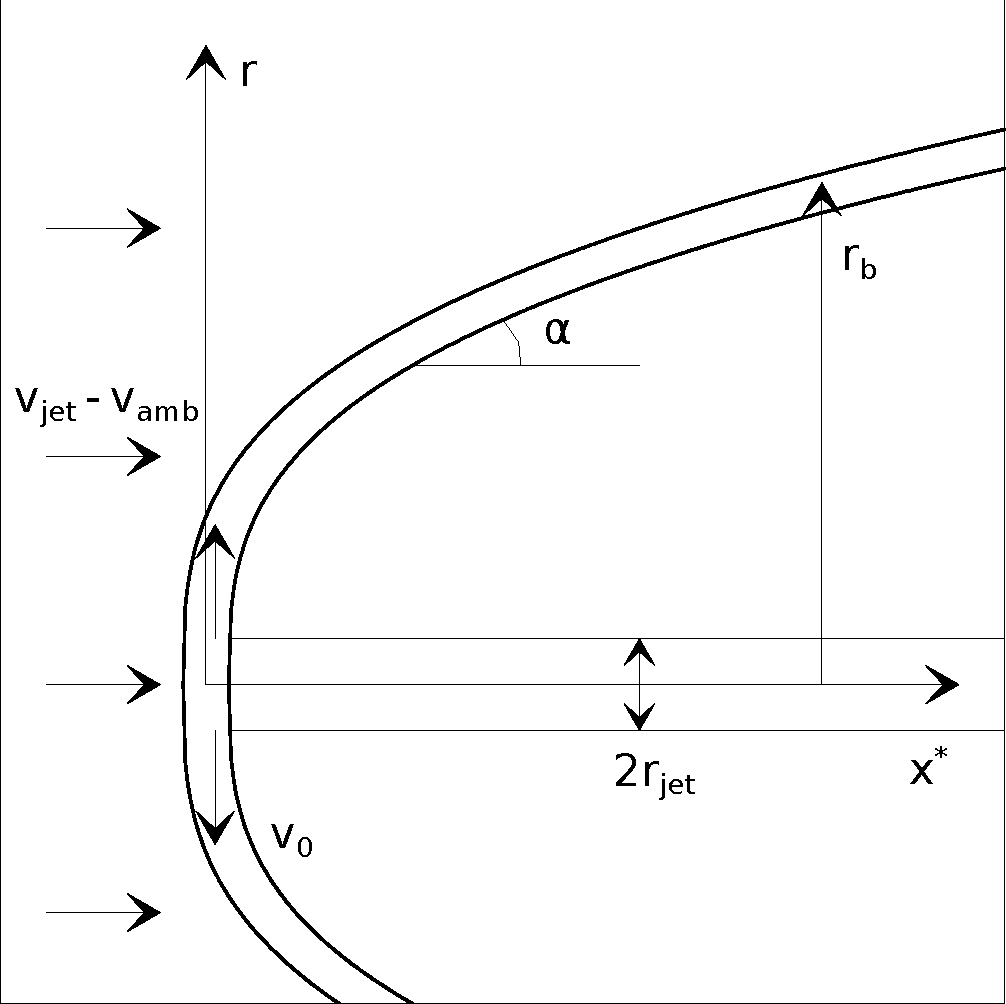
\includegraphics[width=0.75\textwidth]{figures/bowshock_scheme.pdf}\\
%\includegraphics[width=\textwidth]{bschem.pdf}
\caption[Schematic diagram of the thin shell bowshock model]{{\bf Extended Data Fig.\ 7: Schematic diagram of the thin shell bowshock model.} The bowshock is seen in a reference system moving at the velocity $v_{\rm jet}$ of the working surface. The cylindrical jet beam (of diameter $2\,r_{\rm jet}$) stops in the working surface, as it interacts with the impinging ambient gas (moving to the right at a velocity $v_{\rm jet}-v_{\rm amb}$). We show a cylindrical coordinate system $(x^*,r)$, where $r$ is the cylindrical radius and $x^*$ the distance measured from the head of the working surface towards the outflow source. The working surface ejects material sideways at a velocity $v_0$ (which is approximately equal to the post-cooling region sound speed of $\sim 10$~km~s$^{-1}$). This sideways ejection interacts with the impinging ambient gas, forming a thin shell bowshock that has a well defined locus $r_b(x^*)$, and locally has a slope $\tan\alpha=dr_b/dx^*$.
\label{a1}
}
\end{center}
\end{figure}

%The flow structure seen in a reference frame ($\^x, r$) moving with the working surface is shown in Extended Data Fig.~7. The bowshock propagates in the $z$-axis direction, which is related with the $\^x$-axis as $\^x=z_j-z$, where $z_j$ the distance of the working surface from the source.



The shape of the bowshock wings is determined by the interaction of the material ejected sideways by the working surface (with a velocity $v_0$ and mass rate ${\dot m_0}$) with the streaming ambient material (which impinges on the jet head with a density $\rho_{\rm amb}$ and velocity $v_{\rm jet}-v_{\rm amb}$, 
 %see Fig.~\ref{a1}).
see Extended Data Fig.~7). We assume that the jet material (ejected sideways by the working surface) and the entrained ambient material form a stationary, well mixed thin shell. This shell has a locus $r_b(x^*)$ 
 %(see Fig.~\ref{a1})
(see Extended Data Fig.~7) that results from the mass and $(x^*,r)$-momentum conservation equations:
\begin{eqnarray}
%\begin{equation}
	{\dot m} & = & {\dot m}_0+\pi r_b^2 \rho_{\rm amb}(v_{\rm jet}-v_{\rm amb})=2\pi r_b \sigma v_t\,, \label{mcon} \\ 
%\end{equation}
%\begin{equation}
	{\dot \Pi}_{x^*} & = & \pi r_b^2\rho_{\rm amb}(v_{\rm jet}-v_{\rm amb})^2={\dot m} v_{x^*}\,, \label{xcon} \\
%\end{equation}
%\begin{equation}
  {\dot \Pi}_r & = & {\dot m_0}v_0={\dot m}v_r\,,
  \label{rcon}
%\end{equation}
\end{eqnarray}
where ${\dot m}$, ${\dot \Pi}_{x^*}$ and ${\dot \Pi}_r$ are the mass, $x^*$-momentum and $r$-momentum rates flowing along the thin shell up to a given value of $x^*$, and $v_t$, $v_{x^*}$ and $v_r$ are the components of the velocity of the well mixed material within the shell along the shell surface, and along the $x^*$- and $r$-axes, respectively. Finally, $\sigma$ (see the last term of equation (\ref{mcon})) is the surface density of the thin shell.

\begin{eqnarray}
	v_{x^*} & = &\frac{\pi r_b^2\rho_{\rm amb}(v_{\rm jet}-v_{\rm amb})^2}{\dot m_0+\pi\rho_{\rm amb}(v_{\rm jet}-v_{\rm amb})r_b^2}\,, \label{vx} \\ 
 %\end{equation}
 %\begin{equation}
	v_r & = & \frac{{\dot m}_0v_0}{\dot m_0+\pi\rho_{\rm amb}(v_{\rm jet}-v_{\rm amb})r_b^2}\,.
  \label{vr}
\end{eqnarray}
One then combines these two equations to obtain the differential equation:
\begin{equation}
	\frac{dr_b}{dx^*}=\tan \alpha=\frac{v_r}{v_{x^*}}=\frac{{\dot m}_0v_0}
	{\pi r_b^2\rho_{\rm amb}(v_{\rm jet}-v_{\rm amb})^2}\,,
    \label{drb}
\end{equation}
where $\alpha$ is the angle between the jet axis and the local tangent to the bow surface. Equation (\ref{drb}) can be directly integrated to obtain the shape of the bowshock wings:
 % which can be directly integrated to obtain the shape of the bowshock wings:
\begin{equation}
	r_b(x^*)=\left(L_0^2\, x^*\right)^{1/3},
  \label{rb}
\end{equation}
with
\begin{equation}
	L_0\equiv \sqrt{\frac{3{\dot m}_0 v_0}{\pi\rho_{\rm amb}(v_{\rm jet}-v_{\rm amb})^2}}\,.
  \label{l0}
\end{equation}


The free parameters of the model are: (i) the size scale $L_0$ of the bowshock (see equation (\ref{l0})), (ii) $v_{\rm jet}$ and $v_{\rm amb}$ (the velocities of the jet head and of the medium into which it is travelling), (iii) $v_0$ (the velocity at which the jet material is ejected sideways by the internal working surface)%or the dimensionless parameter $\gamma$ (see equation (\ref{gam}))
, and (iv) the inclination angle $i$
 %orientation angle 
of the outflow direction with respect to the LOS.

Each family of rings is assumed to trace a bowshock whose parameters are obtained as those of the model that best matches the properties of the elliptical fits to the observed rings in the channel maps, in terms of mean ring radius and relative LOS velocity as a function of projected distance to the source on the plane of the sky, $x'$. For the best defined families of rings, we obtain $L_0=0.38\arcsec$, $v_0=20~\kms$, $v_{\rm jet}=110~\kms$ (Rings II); $L_0=0.50\arcsec$, $v_0=17~\kms$, $v_{\rm jet}=109~\kms$ (Rings III); and $L_0=1.80\arcsec$, $v_0=25~\kms$, $v_{\rm jet}=133~\kms$ (Rings VI). In all cases, $i=20^\circ$ and $v_{\rm amb} \simeq 0~\kms$ (see Fig.~\ref{fig:modeleli} and Extended Data Table 1).



\begin{figure*}[p!]
\begin{center}
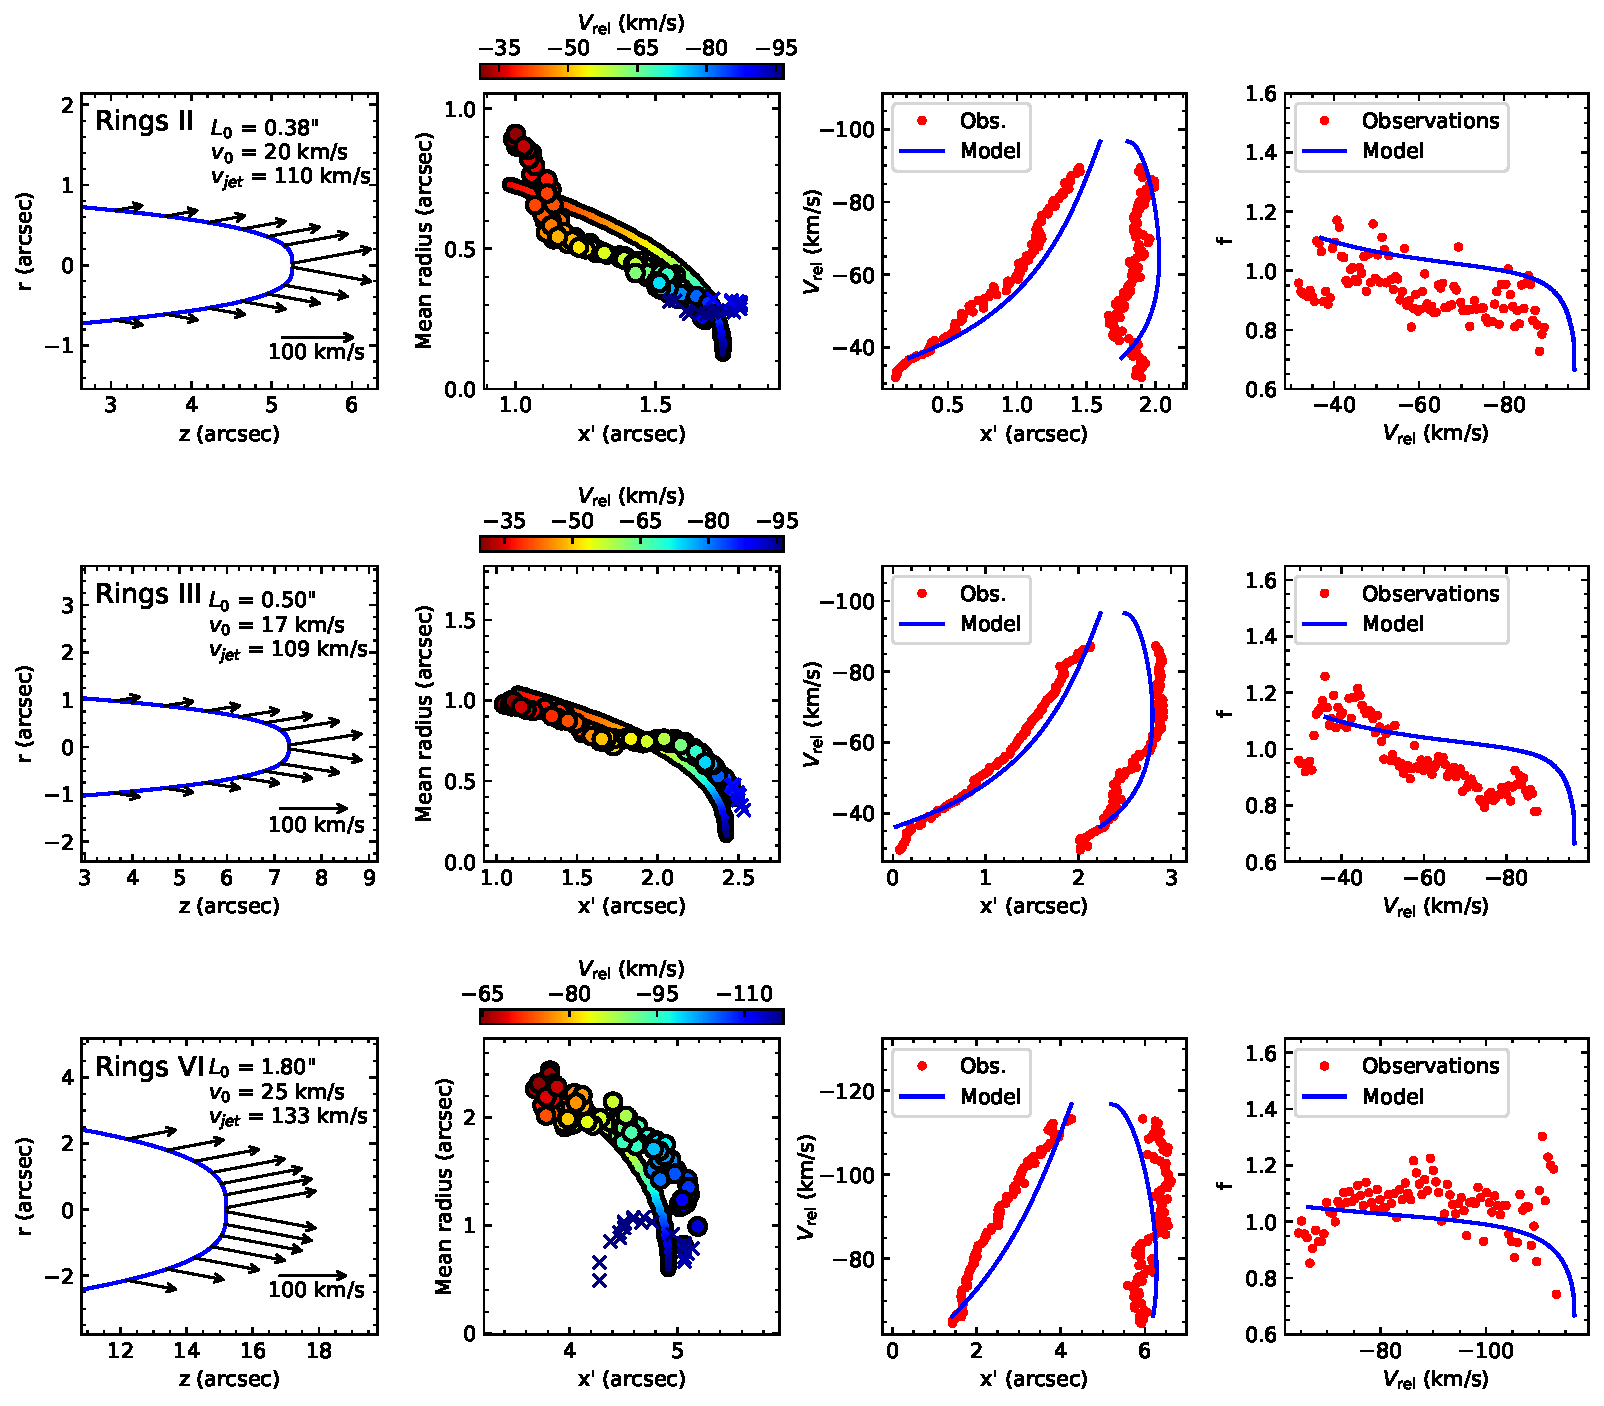
\includegraphics[width=1.0\textwidth]{figures/bowshock_fitresults.pdf}
\end{center}
\end{figure*}
\begin{figure}[p!]
\begin{center}
\caption[Comparison of the bowshock model results with the elliptical fits to the observations]{{\bf Comparison of the bowshock model results with the elliptical fits to the observations.} 
The rows correspond to families II, III and VI, respectively, from top to bottom. 
{\bf First column:} Depiction of the shape and velocity field of the bowshock model, where $z$ is the symmetry axis (whose origin is VLA 4B) and $r$ is the cylindrical radius of the bowshock. The main parameters of the model, the characteristic scale ($L_0$), the velocity at which the jet material is initially ejected sideways by the working surface ($v_0$), and the velocity of the internal working surface along the $z$-axis ($v_{\rm jet}$), are listed in the top right corner of the panels. The distance from the source to the internal working surface ($z_{\rm ws}$) is taken as the position of the head of the family.
In all cases, the inclination angle is $i=20^\circ$, and the velocity of the medium into which the jet is traveling is $v_{\rm amb}\simeq0~\kms$ (see Methods and Extended Data Table~1).
{\bf Second column:} Observed (dots indicate rings and x symbols indicate filled emission of the head) and model (continuum line) bowshock radius as a function of the projected distance to VLA 4B. Velocities are indicated in a color scale. 
{\bf Third column:} Observed (red dots) and model (blue line) position-velocity diagram for the rings (excluding the heads).
{\bf Fourth column:} Observed (red dots) and model (blue line) elongation factor of the rings ($f$), taken as the ratio of the ring axes along the longitudinal and tranverse directions.
 %The origin of distances is VLA~4B.
All velocities are LOS velocities relative to the velocity of VLA~4B.
 %The model parameters are (see Methods): the characteristic scale ($L_0$), the velocity of the internal working surface along the $z$-axis ($v_{\rm jet}$), the velocity of the medium into which the jet is traveling ($v_{\rm amb}$), the velocity at which the jet material is initially ejected sideways by the working surface ($v_0$), 
 %transverse velocitiy ($v_0$),
%and the inclination angle ($i$). 
 %The values of the model parameters are: $L_0=0.38''$, $v_{\rm jet}=110$ \kms, $v_0=20$ \kms, and $z_{\rm ws}=2.63''$ (family II); $L_0=0.5''$, $v_{\rm jet}=109$ \kms, $v_0=17$ \kms, and $z_{\rm ws}=4.39''$ (family III); $L_0=1.8''$, $v_{\rm jet}=133$ \kms, $v_0=25$ \kms, and $z_{\rm ws}=3.80''$ (family VI). In all cases, $i=20^\circ$ and $v_{\rm amb}=0$. 
 %the velocity of the medium into which the jet is traveling is negligible.
 Additional plots of the angle between the position vector and the symmetry axis predicted by the models are shown in Extended Data Fig.~6. 
 %{\em We note that the analytic solution used here predicts a length of the bowshock shorter that observed, however the numerical simulations predict larger bowshocks, in accordance with what is observed.}
 \label{fig:modeleli}} %Figure 5old = Fig 4new
\end{center}
 \end{figure}



\begin{figure}[p!] 
\begin{centering}
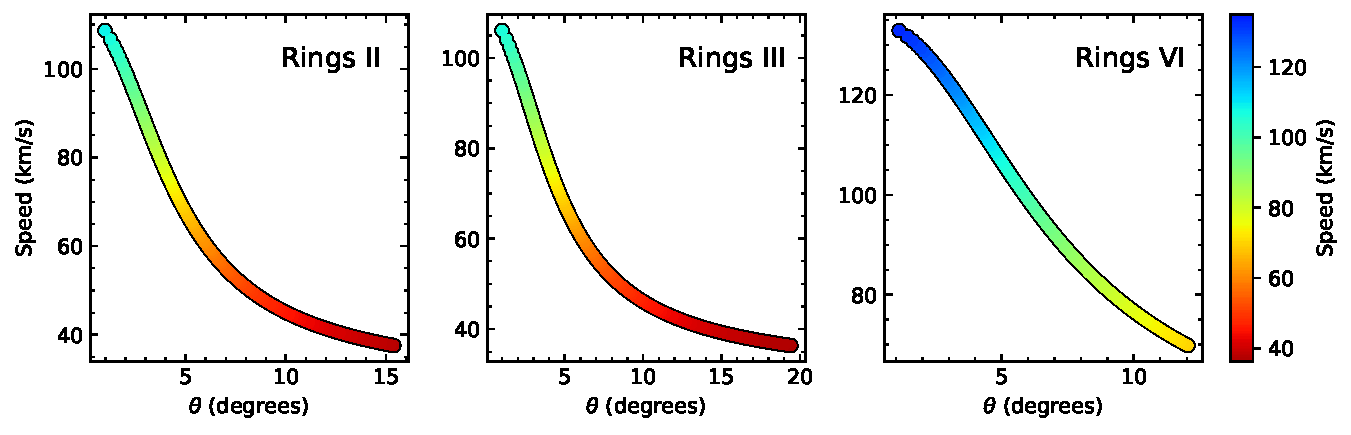
\includegraphics[width=\textwidth]{figures/speed_theta_bowshock.pdf} 
\caption[Velocity as a function of the polar angle for the bowshock model]{{\bf Extended Data Fig.\ 6: Velocity as a function of polar angle for the bowshock model.} Speed of the bowshock material as a function of the polar angle, $\theta$, defined as the angle of the position vector with respect to the symmetry axis of the shell, $z$, for families II, III, and VI. An inclination angle  $i=20^\circ$ is assumed for all the plots. The model parameters for families II, III, and VI are presented in Extended Data Table 1.
 Note that the bowshock model naturally explains the increase of velocity near the symmetry axis.
\label{fig:v_theta}
}
\end{centering}
\end{figure}



\subsection{Derivation of the density of the ambient gas and mass rates}

The density of the ambient gas, $\rho_{\rm amb}$, can be estimated from the mass of the bowshock shell, $M$ (i.e., the mass of a given family of rings), which can be measured from the observations (see ``Determination of the mass'' in Methods). Once $\rho_{\rm amb}$ is known, the mass rate of jet material initially ejected sideways by the working surface, $\dot{m}_0$, and the mass rate of ambient material being incorporated, $\dot{m}_{\rm amb}$, can be derived.

%The mass of the bowshock shell, $m$ (i.e., the mass of a given family of rings), which can be estimated from the observations, (see ``Determination of the mass'' in Methods), can be related to the mass rate of jet material initially ejected sideways by the working surface, $\dot{m}_0$, the density of the ambient gas, $\rho_{\rm amb}$, and the mass rate of material incorporated from the ambient, $\dot{m}_{\rm amb}$.

 %We obtain $\rho_w$ as a function of $m$ by integrating the mass rate $\dot{m}$, given by equation (\ref{mcon}; 48). 

In the narrow jet regime ($r_{\rm jet}\ll L_0$), the mass of the shell can be obtained by integrating the mass rate flowing along the shell, $\dot m=\dot{m}_0+\dot{m}_{\rm amb}$ (equation (\ref{mcon})), over the whole lifetime of the bowshock: 
%up to maximum bowshock radius $r_{b,f}$: 
\begin{equation}\label{eq:intmass_mr}
	M=\int_{t_0}^{t_f}\dot{m}\, dt = \int_0^{r_{f}}\dot{m} \frac{dr_b}{v_r}, 
\end{equation}
%where , estimated as the dynamical time, $t_{dyn}$, of the points at the maximum bowshock radious $r_{b,f}$.
where $t_f-t_0$ is the time elapsed since the bowshock was originated, $v_r=dr_b/dt$, 
and $r_f \equiv r_{b}(t_f)$ is the observed maximum radius, corresponding to the outer edge of the bowshock shell.

From the conservation of $r$-momentum, given by equation (\ref{rcon}), we have 
% where we used, combining equations (\ref{mcon}; 48) and (\ref{vr}; 52), from equation (\ref{rcon}; 50)
\begin{equation}
	v_r = \frac{\dot{m}_0 v_0}{\dot{m}},
\end{equation}
and substituting in equation (\ref{eq:intmass_mr}), we obtain
\begin{equation}\label{eq:intmass_m0}
 %m=\int_0^{r_{b,f}}\frac{(\dot{m})^2}{\dot{m}_0 v_0}\, dr_b.
M=\int_0^{r_{f}}\frac{\dot{m}^2}{\dot{m}_0 v_0}\, dr_b.
\end{equation}
From the definition of $L_0$ (equation (\ref{l0})), the mass conservation equation (equation (\ref{mcon})) can be written as:
\begin{equation}\label{eq:mdotm0}
	\dot{m} = \dot{m}_0\left[1+\frac{3}{\gamma}\left(\frac{r_b}{L_0}\right)^2\right],
\end{equation}
with
\begin{equation}
	\gamma\equiv \frac{v_{\rm jet}-v_{\rm amb}}{v_0}\,,
  \label{gam}
\end{equation}
and substituting in equation (\ref{eq:intmass_m0}),
\begin{equation}
M=\int_0^{r_{f}}\frac{\dot{m}_0}{v_0}\left[1+\frac{3}{\gamma}\left(\frac{r_b}{L_0}\right)^2\right]^2\, dr_b.
\end{equation}
 %Using the change of variable $u=\sqrt{\frac{3}{\gamma}}\frac{r_b}{L_0}$ and resolving the integral:
 Using the change of variable $u=(3/\gamma)^{1/2} (r_b/L_0)$ %{\color{red} $u=3^{1/2} \gamma^{-1/2} L_0^{-1} r_b$}
and resolving the integral:
\begin{equation}
M=\frac{\dot{m}_0L_0}{v_0}\left(\frac{\gamma}{3}\right)^{1/2}\int_0^{u_f}\left(1+u^2\right)^2\, du= \frac{\dot{m}_0L_0}{v_0}\left(\frac{\gamma}{3}\right)^{1/2}\left(\frac{u_f^5}{5} + \frac{2u_f^3}{3} + u_f\right),
\end{equation}
where $u_f=(3/\gamma)^{1/2} (r_{f}/L_0)$. 

 %$u_f=\sqrt{\frac{3}{\gamma}}\frac{r_{b,f}}{L_0}$. 

Combining equation (\ref{l0}) and (\ref{gam}), 
 %we can write $m$ as a function of $\rho_{\rm amb}$:
%\begin{equation}
 %m= \pi\rho_{\rm amb}\, \gamma^{5/2}\left(\frac{L_0}{\sqrt{3}}\right)^3\left(\frac{u_f^5}{5} + \frac{2u_f^3}{3} + u_f\right).
 %m= 3\pi\rho_{\rm amb}\, \left(\frac{\gamma}{3}\right)^{5/2} L_0^3 \left(\frac{u_f^5}{5} + \frac{2u_f^3}{3} + u_f\right).
%\end{equation}
%Thus, 
we can calculate the density of the ambient medium, $\rho_{\rm amb}$, as a function of the mass of the shell, $M$, as:
\begin{equation}\label{eq:rhow_mr}
 \rho_{\rm amb} = M \left[3\pi \left(\frac{\gamma}{3}\right)^{5/2} L_0^3 
 \left(\frac{u_f^5}{5} + \frac{2u_f^3}{3} + u_f\right)\right]^{-1}.
	%\rho_{\rm amb} = m \left[\pi \gamma^{5/2} \left(\frac{L_0}{\sqrt{3}}\right)^3 \left(\frac{u_f^5}{5} + \frac{2u_f^3}{3} + u_f\right)\right]^{-1}.
\end{equation}
Note that, when $r_{f}\gg L_0$ ($u_f\gg 1$), $\rho_{\rm amb}$ can be approximated as:
\begin{equation}
	\rho_{\rm amb} \simeq M \left[3\pi \left(\frac{\gamma}{3}\right)^{5/2} L_0^3 \left(\frac{u_f^5}{5}\right)\right]^{-1} = \frac{5}{3\pi} \frac{M\, L_0^2}{r_{f}^5}. %\frac{5 L_0^2\, m}{3\pi\, r_f^5}.  %\frac{5}{3\pi}  m\frac{L_0^2}{r_{f}^5}.
\end{equation}

Once we have an estimate of $\rho_{\rm amb}$, we can calculate from equation (\ref{eq:mdotm0}) the mass rate contribution of the jet to the bowshock, $\dot{m}_0$, as:
\begin{equation}\label{eq:mdot0_rhow}
	\dot{m}_0 = \rho_{\rm amb}\frac{\pi (v_{\rm jet}-v_{\rm amb})^2L_0^2}{3v_0},
\end{equation}
and the contribution of the ambient gas, $\dot{m}_{\rm amb}$, to the mass rate of mixed jet+ambient material flowing along the bowshock up to a radius $r_b$, is given by:
\begin{equation}\label{eq:mw}
	\dot{m}_{\rm amb} = \pi \rho_{\rm amb} (v_{\rm jet}-v_{\rm amb}) r_b^2.
\end{equation}

Note that, from equations (\ref{eq:mdot0_rhow}) and (\ref{eq:mw}), the ratio of the jet mass rate to the ambient mass rate up to a given radius $r_b$ is given by
\begin{equation}
	\frac{\dot{m}_0}{\dot{m}_{\rm amb}} = \frac{\gamma}{3}\left(\frac{L_0}{r_b}\right)^2,
\end{equation}
%By comparing the two terms of the mass rate in equation (\ref{eq:mdotm0}),
so only the tip of the bowshock, where $r_b<L_0 (\gamma/3)^{1/2}$, is dominated by ejected jet material. 

Evaluating equation (\ref{eq:mw}) at the maximum radius of the shell, $r_{f}$, we can obtain the mass rate of ambient material 
 %from the environment
 incorporated to the whole bowshock:
\begin{equation}\label{eq:mw_f}
	\dot{M}_{{\rm amb}}=\pi \rho_{\rm amb} (v_{\rm jet}-v_{\rm amb}) r_{f}^2. 
\end{equation}

From the bowshock parameters and the observed mass of each family, $M$ (see above section in Methods and extended Data Table 1), 
 %The results for 
$\rho_{\rm amb}$, $\dot{m}_0$, and $\dot{M}_{{\rm amb}}$ can be obtained from equations (\ref{eq:rhow_mr}), (\ref{eq:mdot0_rhow}), and (\ref{eq:mw_f}), respectively. The results are shown in Extended Data Table~1.  %for Rings II, III, and VI. 
We obtain densities $\rho_{\rm amb}$ = 4.6$\times$10$^{-19}$, 2.2$\times$10$^{-19}$, and 2.2$\times$10$^{-20}$~g~cm$^{-3}$ for Rings II, III, and VI, respectively. Thus, we derive decreasing values of $\rho_{\rm amb}$ with distance from the source (Rings II are the closest to the source of the three families, and Rings VI are the farthest), which is physically consistent with the source being an embedded object, located in the central, denser region of a molecular core.

We obtain $\dot{m}_0$ = 1.4$\times$10$^{-6}$, 1.2$\times$10$^{-6}$, and 1.7$\times$10$^{-6}~M_\odot~\mathrm{yr}^{-1}$ for Rings II, III, and VI. Taking $\dot{m}_0$ as a good estimate of the mass-loss rate of the jet , we infer $\dot{M}_\mathrm{jet}$ = 1-2$\times$10$^{-6}~M_\odot~\mathrm{yr}^{-1}$. It is worth noting that, since the mass accretion rate inferred for VLA 4B is $\dot{M}_\mathrm{acc}$ = 0.8-1.3 $\times$ 10$^{-5}~M_\odot~\mathrm{yr}^{-1}$ (see Methods), we obtain an ejection to accretion ratio of $\dot{M}_\mathrm{jet}/\dot{M}_\mathrm{acc}\simeq 0.1$, consistent with the typical value in outflows.

Regarding the mass rate of ambient material that is incorporated into the bowshock, we obtain $\dot{M}_{{\rm amb}}$ = 2.9$\times10^{-6}$, 2.4$\times10^{-6}$, and 1.6$\times10^{-6}~M_\odot~\mathrm{yr}^{-1}$ for Rings II, III, and VI, respectively. Also, we see that, while for Rings II and III $\dot{M}_{{\rm amb}} \simeq 2\,\dot{m}_0$, for Rings VI we obtain $\dot{M}_{{\rm amb}} \simeq \dot{m}_0$. Since Rings VI are the most distant, it seems possible that this decrease in the relative contribution of the ambient gas to the bowshock mixed material is a consequence of the observed decrease in the surrounding ambient density, $\rho_{\rm amb}$, with distance. Nonetheless, for Rings VI, the rings with largest radii are faint and difficult to identify, so we could be missing a significant part of the mass that is predominantly composed by ambient material.

\begin{table}[p!]
{\footnotesize
\begin{tabular}{lccccccccc}
\hline
& 
\multicolumn{1}{c}{$L_0$} & 
\multicolumn{1}{c}{$v_0$} & 
\multicolumn{1}{c}{$v_{\rm jet}$} & 
\multicolumn{1}{c}{$z_{\rm ws}$} & 
\multicolumn{1}{c}{$M$} & 
\multicolumn{1}{c}{$\rho_{\rm amb}$} &
\multicolumn{1}{c}{$\dot{m}_0$} & 
\multicolumn{1}{c}{$\dot{M}_{{\rm amb}}$} \\
Family & 
\multicolumn{1}{c}{(arcsec)} & 
\multicolumn{1}{c}{(km~s$^{-1}$)} & 
\multicolumn{1}{c}{(km~s$^{-1}$)} & 
\multicolumn{1}{c}{(arcsec)} & 
\multicolumn{1}{c}{($M_\odot$)} & 
\multicolumn{1}{c}{(g~cm$^{-3}$)} & 
\multicolumn{1}{c}{($M_\odot$~yr$^{-1}$)} &
\multicolumn{1}{c}{($M_\odot$~yr$^{-1}$)} \\
\hline
II & 0.38 & 20 & 110 & 5.26  & $2.4\times10^{-4}$ & $4.6\times10^{-19}$  & 1.4$\times10^{-6}$ & 2.9$\times10^{-6}$ \\
III& 0.50 & 17 & 108 & 7.31  & $3.1\times10^{-4}$ & $2.2\times10^{-19}$  & 1.2$\times10^{-6}$ & 2.4$\times10^{-6}$ \\
VI & 1.80 & 25 & 132 & 14.61 & $4.0\times10^{-4}$ & $2.2\times10^{-20}$ & 1.7$\times10^{-6}$ & 1.6$\times10^{-6}$ \\
\hline
\end{tabular}
\caption[Bowshock model parameters for families of Rings II, III, and VI.]{{\bf Bowshock model parameters for families of Rings II, III, and VI.} $L_0$ is the characteristic scale, $v_0$ the initial velocity at which jet material is ejected sideways, $v_{\rm jet}$ the velocity of the working surface, $z_{\rm ws}$ the position of the head of the family, $M$ the mass measured from the observations, $\rho_{\rm amb}$ the density of medium into which the jet is traveling, $\dot{m}_0$ the mass-rate of jet material ejected sideways by the internal working surface, and $\dot{M}_{\rm amb}$ the mass-rate of ambient material that is incorporated into the bowshock shell. In all cases, the inclination angle is $i=20^\circ$, and the velocity of the ambient medium is $v_{\rm amb} \simeq 0$ \kms. The adopted distance is $D=300$ pc \citep{ortiz-leon2018, gaia2023}.}
}
\end{table}



\subsection{Calculation of the emission of the channel maps}

Finally, we consider that the velocity along the thin shell can be written as $v_t=v_{x^*}\cos\alpha+v_r\sin\alpha$, and use equations (\ref{mcon}) and (\ref{vx})-(\ref{drb}) to calculate
the surface density of the shell as
% \begin{equation}
%   \sigma=\left(\frac{\rho_w}{2R_b}\right)
%   \frac{\left(L_0^2 \gamma/3+R_b^2\right)^2}{R_b^2\cos\alpha+(L_0^2/3)\sin\alpha}\,,
%   \label{sig}
% \end{equation}
\begin{equation}
	\sigma=\frac{1}{2}~\rho_{\rm amb}\cos\alpha\left(\gamma\tan\alpha + 1\right)^2 r_b\,,
	\label{sig}
\end{equation}
with
\begin{equation}
	\cos\alpha=\left(1+\frac{L_0^4}{9r_b^4}\right)^{-1/2},
  \label{cal}
\end{equation}
\begin{equation}
	\tan\alpha = \frac{1}{3}\left(\frac{L_0}{r_b}\right)^2,
\end{equation}
% \begin{equation}
%   \sin\alpha=\left(1+\frac{9r_b^4}{L_0^4}\right)^{-1/2}
%   \label{sal}
% \end{equation}
We then have a full solution giving the shape (equation (\ref{rb})), velocity (equations (\ref{vx}) and (\ref{vr})) and surface density (equation (\ref{sig})) for a thin shell bowshock flow. In practice, a thermal+turbulent velocity dispersion, $v_T$, is expected to be present so that the surface density is spread over a range of velocities, which is taken into account when calculating the distribution in velocity channels. In our case, we find a 3D velocity dispersion $v_T\simeq 2~\kms$, which corresponds to a LOS velocity dispersion of $\simeq 1.2~\kms$. 

Once we know the shape of the bowshock shell, with the velocity and surface density at all its points, we can obtain their projected positions on the plane of the sky and their LOS velocities. 
%In this way, we can assign each point of the shell to a pixel in a channel map, obtaining the mass and columnar density for each of the pixels and channels of the model. 
In this way, we can assign each point of the shell to a pixel in a given channel map of width $\Delta v_{\rm ch}$, obtaining the mass and column density for each of the pixels of the model channels.
 From the CO column density, obtained through its abundance relative to H$_2$, we can derive the CO optical depth and intensity predicted by the model using equations~(\ref{eq:nmol2}) and (\ref{eq:i1}), respectively. Finally, channel maps directly comparable with observations can be simulated by convolving the intensities with the appropriate beam. 

\clearpage
\begin{figure}[p!]
\begin{center}
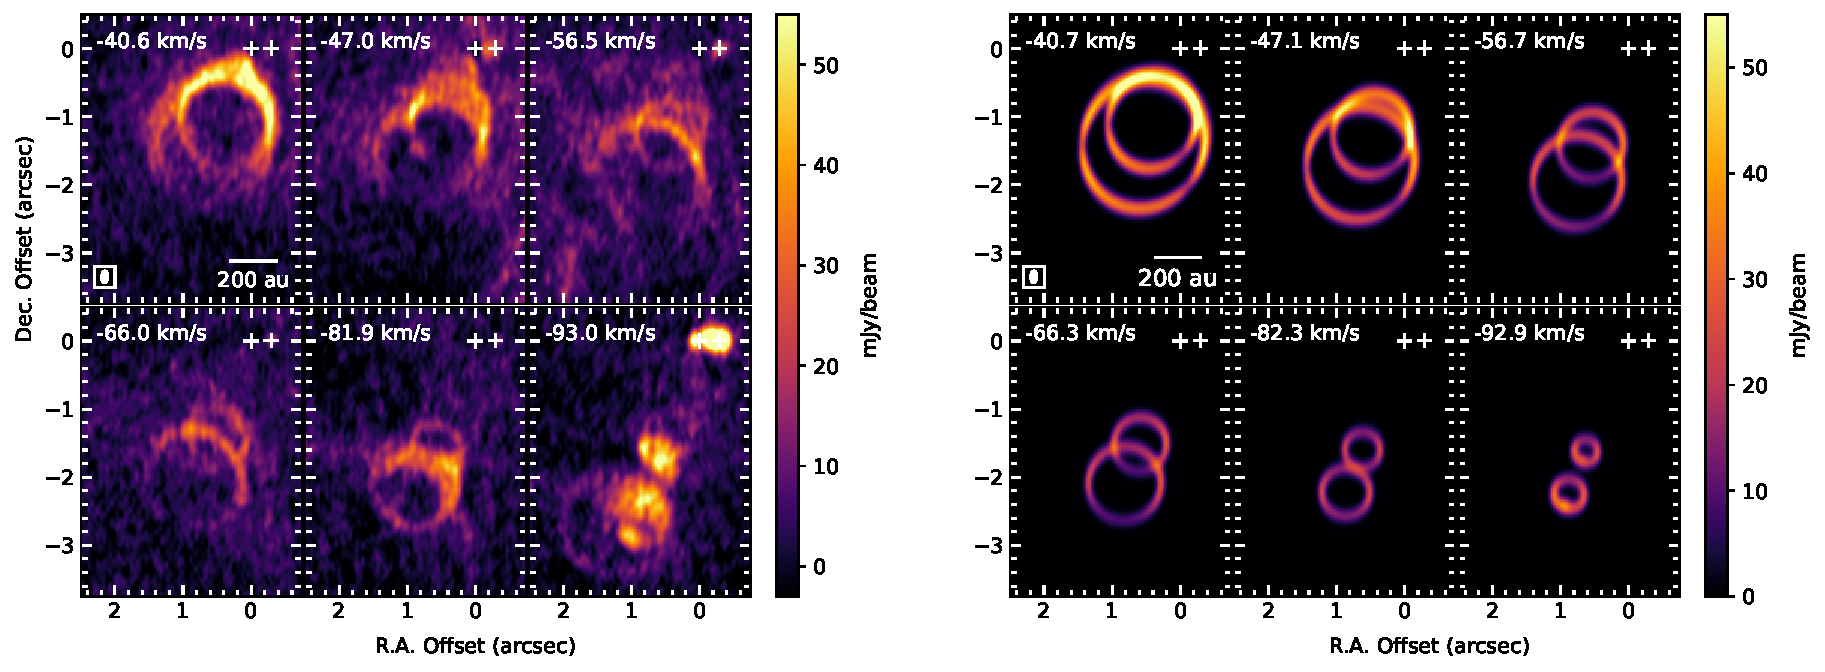
\includegraphics[width=1.0\textwidth]{figures/obs_model_channels.pdf}
%\caption{{\bf Comparison of observed and bowshock model spectral channel images.} Comparison of a set of observed (left) and bowshock model (right) spectral channel images corresponding to ring families II (the northernmost) and III (the southernmost), which are the two families with the best observational data. Left panels represent the observed intensity, in mJy beam$^{-1}$, while the right panels show the model normalized??? column density per velocity bin,???
 %per channel???, 
%in arbitrary units, proportional to the intensity for optically thin isothermal emission. The model parameters are given in Fig.~\ref{fig:modeleli}. The model images have been calculated for a channel width of $\Delta v_{\rm ch}$ = 0.53 \kms\ (the same as in the observed images), assuming a velocity dispersion of $v_T$ = 3 \kms. Offsets are relative to the position of VLA 4B (the easternmost of the two components of SVS~13, indicated by white plus signs). The LOS velocity relative to VLA~4B is indicated in the top left corner of each channel image.
\caption[ Comparison of observed and bowshock model spectral channel images]{{\bf Comparison of observed and bowshock model spectral channel images.} Comparison of a set of observed (left) and bowshock model (right) spectral channel images corresponding to ring families II (the northernmost) and III (the southernmost), which are the two families with the best observational data. The model parameters are given in Fig.~\ref{fig:modeleli} and Extended Data Table 1. The model images have been calculated for a channel width $\Delta v_{\rm ch}$ = 0.53 \kms\ (the same as in the observed images), assuming an intrinsic velocity dispersion (thermal+turbulent) $v_T$ = 2~\kms\ (see Methods). Offsets are relative to the position of VLA 4B (the easternmost of the two components of SVS~13, indicated by white plus signs). The LOS velocity relative to VLA~4B is indicated in the top left corner of each channel image.
}
\label{fig:modelchan}%Figure 4
\end{center}
 \end{figure}

\clearpage
\begin{figure}[p!]
\begin{center}
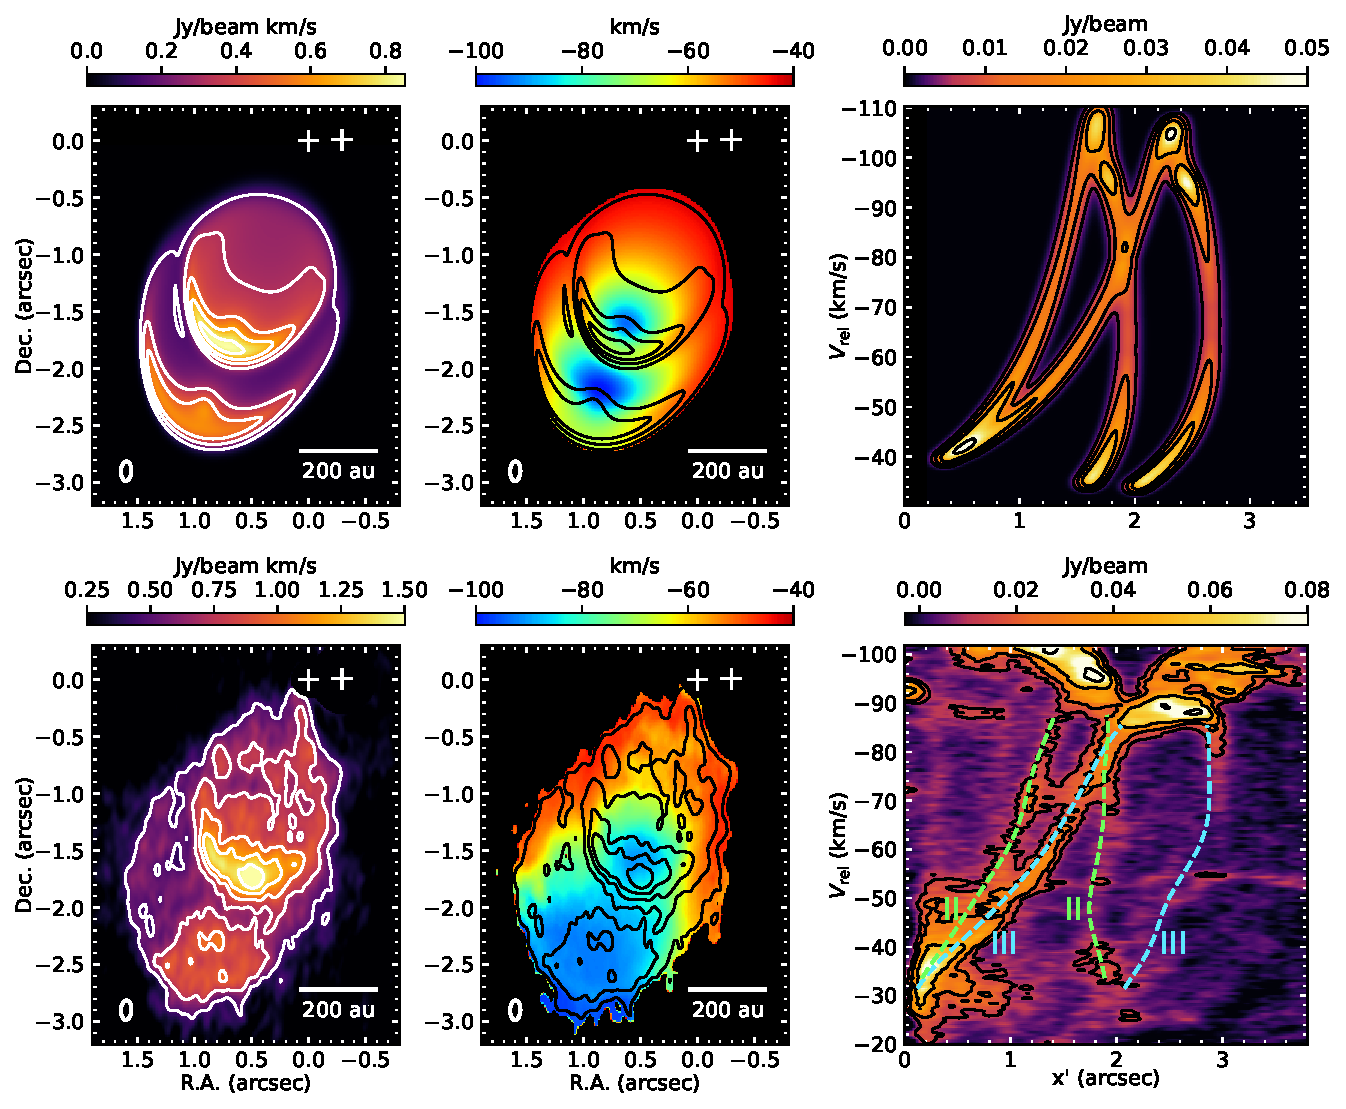
\includegraphics[width=1\textwidth]{figures/obs_model_moments.pdf}
\end{center}
\end{figure}
\addtocounter{figure}{-1}
\begin{figure}[p!]
\begin{center}
\caption[Comparison of the bowshock model with the observed moment images and position-velocity diagrams]{{\bf Comparison of the bowshock model with the observed moment images and position-velocity diagrams.} Comparison of bowshock model (top panels) and observed (bottom panels) zeroth- and first-order moment images, and position-velocity diagrams. The model results correspond to the bowshock model for the families of rings II and III, whose parameters are given in Fig.~\ref{fig:modeleli} and Extended Data Table 1. The LOS velocity range used for model calculations goes from $-$41.6 to $-$112.0 \kms. 
	The observational results correspond to the LOS velocity range where the emission of these two families is dominant, from $-$41.6 to $-$100.8~\kms\ relative to VLA~4B. Nevertheless, some emission from family I is present within $0.5''$ southeast from VLA~4B. The disk emission has been masked in the observed moment images. Yet, the observed emission is stronger than that of the model, since the observations cannot completely isolate the emission from families II and III, and it is likely to include emission from other features. Contour levels in the zeroth-order moments are 4, 6, 8, 10, and 12 times 0.12 Jy~beam$^{-1}~\kms$ for the observations, and 2, 4, 6, 8, and 10 times 0.08 Jy~beam$^{-1}~\kms$ for the model images. The channel width is $0.53~\kms$. The positions of the components of the SVS~13 binary, VLA~4A (west) and VLA~4B (east), are indicated by white plus signs. The contour levels of the position-velocity diagrams (PA = 160$^\circ$, width = $0.1''$) are 5, 10, 20, and 35 times 2.5 mJy~beam$^{-1}$ for the observations, and 2, 5, 10, and 20 times 2.5 mJy~beam$^{-1}$ for the model. Dashed lines in the observed position-velocity diagram indicate the emission from families II and III.
}
\label{fig:modelpv} %Figure 6
\end{center}
\end{figure}




\section{Opacity and ring asymmetry}\label{sec:opacity}

An outstanding feature of the observed rings is that, in general, they appear brighter in the side closer in projection to the origin. This is reproduced by the bowshock model, and can be understood in terms of opacity and beam filling-factor effects due to the geometry of the bowshock relative to the observer, as illustrated in Extended Data Fig.~8.

As shown in the figure (left and central panels in top row), because of the geometry and orientation of the SVS 13 bowshocks with respect to the observer, the emission at a given LOS velocity (i.e., from a given channel map) appears spread over a wide region in the side of the ring closer in projection to the origin (smaller values of $x'$). In the opposite side of the ring (larger values of $x'$), the emission appears projected over a very narrow arcuate region, resulting in a higher intensity (and optical depth) in the emitting pixels (see left panel in the middle row). If the emission was optically thin all over the ring, the flux in each of these two regions would be the same, and the image of the ring would appear symmetric (except for a local effect due to the elongation of the beam; e.g. \citealt{osorio2016}) when convolved with a finite beam (see central panel in the middle row), since the decrease in beam filling-factor due to the smaller number of emitting pixels in the narrow emitting region will be fully compensated by the increase in intensity. However, if the effects of optical depth, $\tau$, are taken into account, the intensity toward a given line of sight is lower by a factor of $[1-\exp{(-\tau)}]/\tau$ with respect to the optically thin regime. When the emission is convolved with a finite beam an asymmetry is produced because the emission in the extended region fills the beam better than in the part of the ring farthest from the origin where the total flux density is lower and distributed in a narrow region (see left and central panels in the bottom row). The last column in the figure includes noise in the model images (middle and bottom) for a more realistic comparison with the observations (top).


\begin{figure*}[p!]
{\centering
 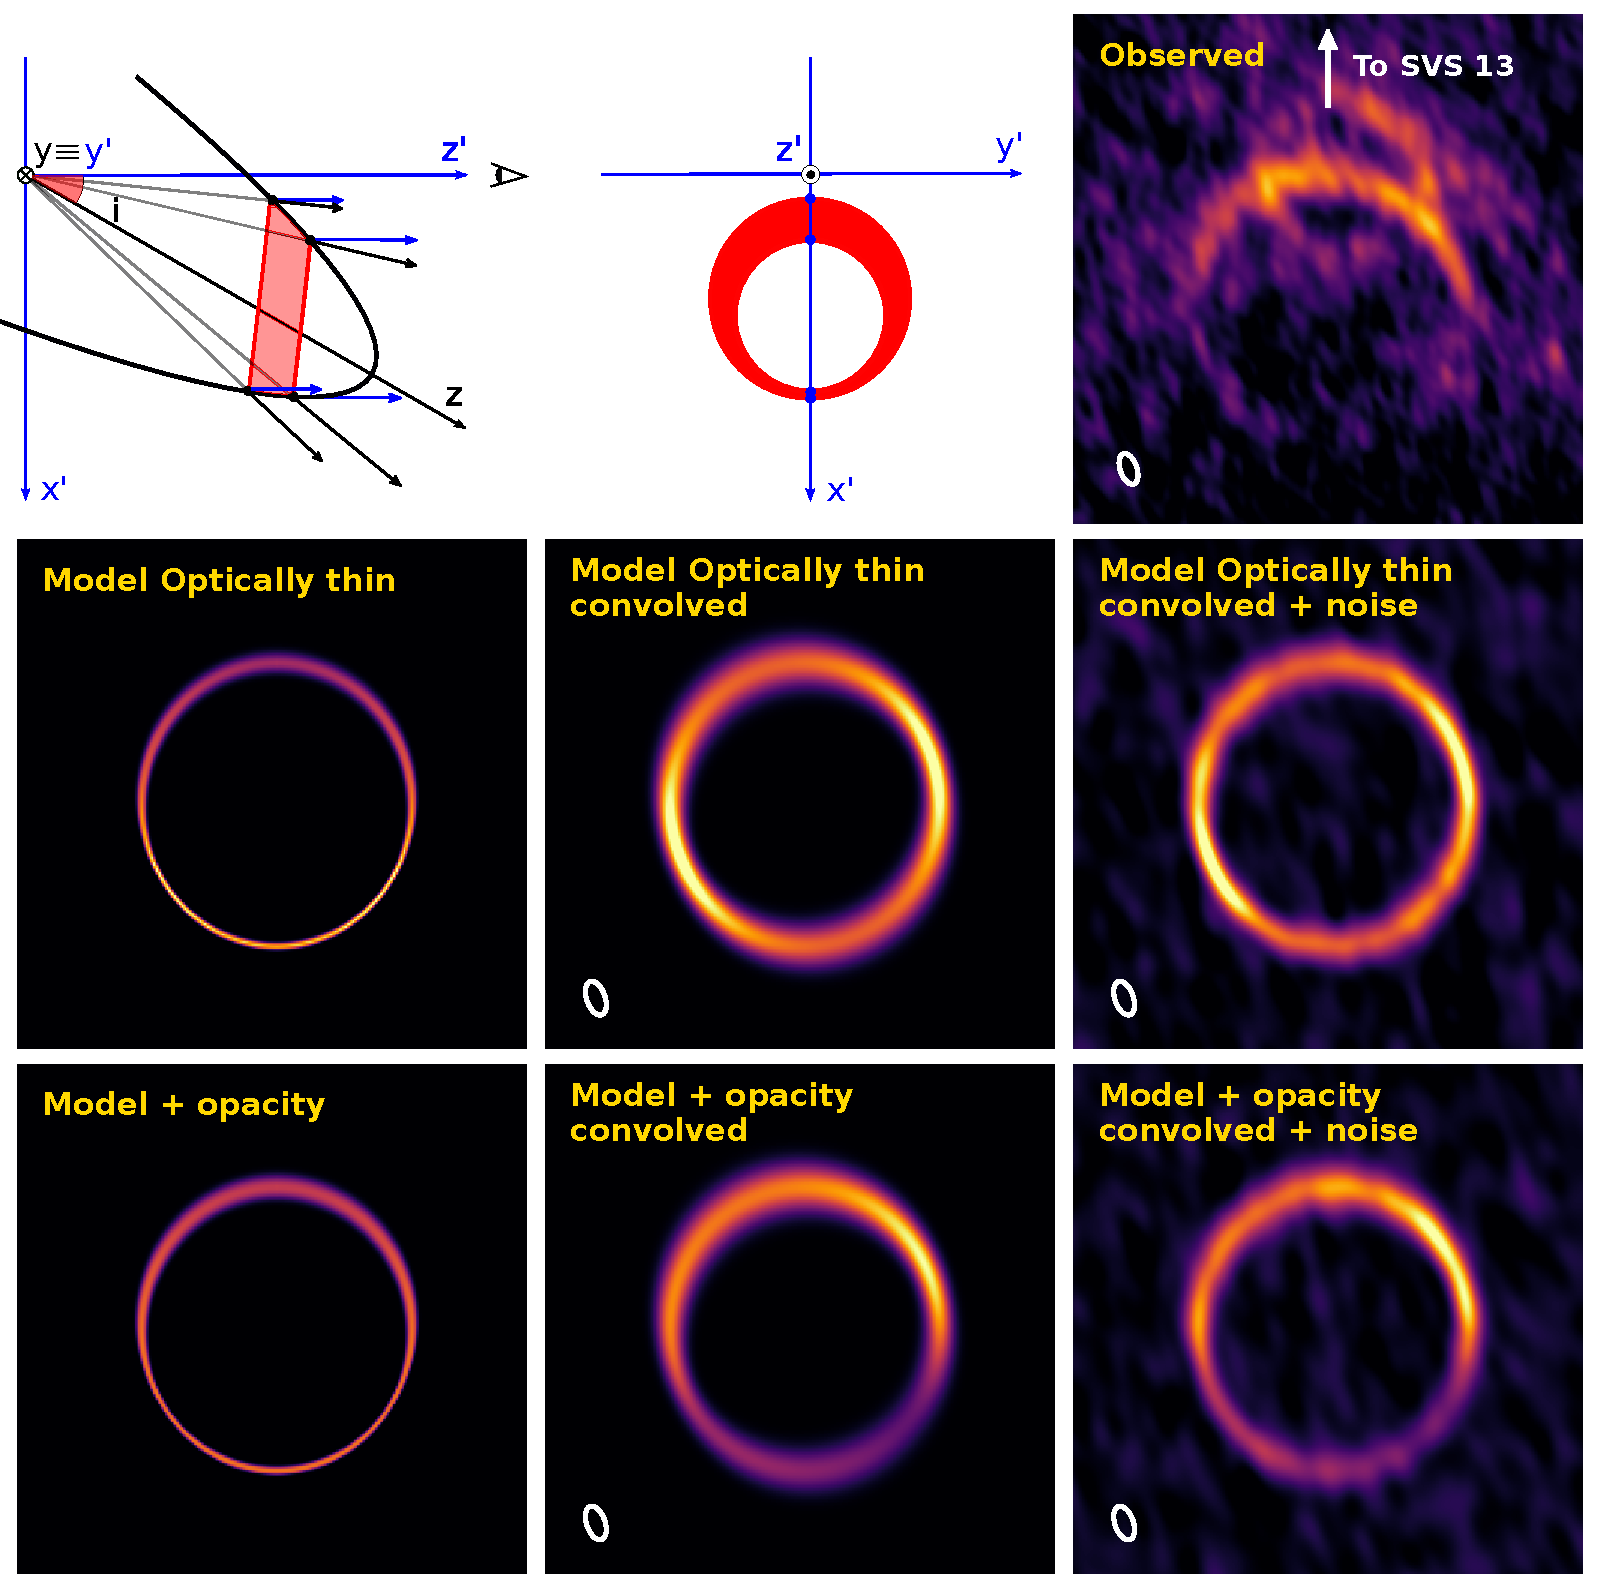
\includegraphics[width=1\textwidth]{figures/extdat_fig8.pdf}\\
}
\end{figure*}
\begin{figure}[p!]
{\bf Extended Data Fig.\ 8: Effect of the optical depth on the observed emission of the rings.} 
{\bf Top left:} Geometry of the bowshock shell, where the black vectors show the shell velocity, the blue vectors show their projections onto the LOS, and the shaded band outlines the spatial extent of the emission in the velocity range of a given channel map. 
{\bf Top center:} Sketch of the corresponding image. The finite range of velocities in the channel maps, makes the ring images to appear with a finite width. Because of the geometry and inclination angle, the emission spreads over a wider area in the sky in the half of the ring closer in projection to the star, while the opposite half of the ring (positions with larger projected distance to the origin) appears narrower because the same range of LOS velocities arises from a much smaller projected area with overlapping lines of sight.
 %Every channel map includes emission with a range of velocities, making the ring images to appear with a finite width. Because of the geometry and inclination angle, the emission spreads over a wider area (and, thus, the intensity is weaker) toward the lines of sight that in projection are closer to the source ($x'$ coordinate closer to the origin), while in the opposite side of the ring (positions with larger projected distance to the origin), it appears narrower (and the intensity stronger) because of the overlapping of the emission at different velocities.
{\bf Top right:} Observed channel image illustrating the asymmetry of the rings in SVS~13, with the side of the ring closest in projection to the star (top of the image) appearing brighter and wider than the opposite side. The image has been rotated so the upper side faces SVS 13.
{\bf Middle row:}
 %Effect of the angular resolution and noise on optically thin ring emission.
 Model images of optically thin rings. At low optical depths, in the upper part of the ring (the side closest to SVS~13 in projection) the emission appears spread over a wider range of radii, and with lower intensity, than in the lower part, where the emitting region is narrower but with higher intensity (left). When convolved with the beam (center), the intensity becomes almost uniform throughout the ring, except for a local increase in intensity near the positions where the beam axis is tangent to the ring, which is a well-known effect due to the variation in the beam filling factor when a narrow ring is observed with an elongated beam \cite{osorio2014}. When noise is added (right), no substantial asymmetries are detected.
 %at the easternmost and westernmost edges, which is a well-known effect due to the variation in the beam filling factor when a narrow ring is observed with a north-south elongated beam \citep{osorio2016}. When noise is added no asymmetries can be detected (right).
{\bf Bottom row:}
 %Combined effect of the angular resolution and optical depth.
 Model images of optically thick rings. When the optical depth is high enough (left), the emission at the top of the ring becomes almost as bright, but more extended, than at the bottom, where intensity increases are hindered by opacity saturation. When convolved with the beam (center), the intensity drops in the lower (narrower) part of the ring, where the beam filling factor is smaller, producing an asymmetry similar to that observed. Inclusion of noise in the model (right) results in remarkable agreement with observations (top right). The assumed velocity dispersion ($v_T$) is 2~\kms, and the assumed channel width is 0.53~\kms\ in all models. %The rest of the model parameters are similar to those used in the family III ring fit (Fig.~\ref{fig:modeleli}).

%
% {\bf Gary comment: Need to say that the black vectors show the shell velocity, blue vectors show the LOS velocity and the bars in the x' direction so the spatial extent of the emission in a given velocity range. And the corresponding image of the emission is shown in the central panel.}
\label{fig:asymmetry}
\end{figure}




\chapter{Summary and conclusions}

The conclusions are

\section{Future work}


\appendix
% \chapter{Appendix: SVS~13 channel maps from ALMA observations}
\chapter{SVS~13 channel maps from ALMA observations}

% \chapter{Appendix: Calculation of model channel maps}
\chapter{Calculation of model spectral cubes}

In this appendix we present the methodology followed in order to compute the spectral cube of a model. This methodology can be applied for any axisymmetric model whose morphology (given by $z$ and $r(z)$), kinematics (given by $v_z(z)$ and $v_r(z)$), and surface density $\sigma(z)$ is known. In the case of the bowshock model, the morphology is given by equation (\ref{rb}), its kinematics by equations (\ref{vx}) and (\ref{vr}), and the surface density by equation (\ref{sig}). The model shape should be projected into the plane of the sky $x'y'$ using the equations (\ref{eq:coord}), while the velocity onto the line of sight velocity $v_{z'}$ with equation (\ref{eq:vzpcoord}), assuming an inclination angle $i$ between the line of sight and the $z$ axis.  

The first step in order to calculate the spectral cube is to grid the space (both the plane of the sky $x'y'$ and the LOS velocity $v_{z'}$): 
\begin{equation}
	(x', y', v_{z'}) \rightarrow (x'_i, y'_i, -v_{\rm ch})
\end{equation}
taking into account sizes of the cells in $\Delta x'$, $\Delta y'$, and $\Delta v_{\rm ch}$. The mass in each cell is given by
\begin{equation}
	\label{eq:masscell}
	m(x'_i, y'_i, v_{\rm ch}) = %\int W_{\rm cube}(x', y', v_{\rm ch}, r_b, \phi) \sigma(r_b) dS = 
	\int^{2\pi}_0\int^{r_f}_{r_{\rm jet}} W_{\rm cube}(x'_i, y'_i, v_{\rm ch}, r, \phi)\, \sigma(r)\, \frac{r\, dr d\phi}{\sin\alpha(r)}\, 
\end{equation}
where $\alpha(r)$ is the angle between the $z$ axis and the shell surface at $r$ and W$_{\rm cube}(x'_i, y'_i, v_{\rm ch}, r, \phi)$ is the weight associated to the cell with spectral cube coordinates ($x'_i$, $y'_i$, $v_{\rm ch}$). $W_{\rm cube}$ can be decompose into the weights of each spectral cube dimension (i.e., $W_{x'}$, $W_{y'}$, and $W_{\rm ch}$) as:
\begin{equation}
    \begin{split}
        &W_{\rm cube}(x', y', v_{\rm ch}, r_b, \phi) = \\
            &W_{x'}(x'_i - x'(r_b, \phi))\, W_{y'}(y'_i - y'(r_b,\phi))\, W_{\rm ch}(v_{\rm ch}+v_{z'}(r_b,\phi))
    \end{split}
\end{equation}
We choose different weightings schemes for the sky coordinates ($x'$ and $y'$ dimensions) and the spectral dimension. For $x'$ and $y'$ dimensions, the weighings $W$ depend on the maximum number of nearest grid points $n$ to which the particle is weighted, and for $n=2$ we have the often called cloud in cell (CIC) scheme:
\begin{equation}
W_{x'}(x'_i - x'(r_b, \phi)) = \left\{ 
  \begin{array}{ c l }
 1 - \frac{|x'_i - x'(r, \phi)|}{\Delta x} & \quad \textrm{if } |x'_i - x'(r, \phi)|< \Delta x' \\
    0                 & \quad \textrm{if } |x'_i - x'(r, \phi)|\geq \Delta x'
  \end{array}
\right.
\end{equation}

\begin{equation}
W_{y'}(y'_i - y'(r, \phi)) = \left\{ 
  \begin{array}{ c l }
 1 - \frac{|y'_i - y'(r, \phi)|}{\Delta y} & \quad \textrm{if } |y'_i - y'(r, \phi)|< \Delta y' \\
    0                 & \quad \textrm{if } |y'_i - y'(r, \phi)|\geq \Delta y'
  \end{array}
\right.
\end{equation}
On the other hand, for the velocity axis, we use the following Gaussian kernel:
\begin{equation}
	W_{\rm ch}(v_{\rm ch} + v_{z'}(r, \phi)) = e^{-\left( \frac{v_{\rm ch}+v_{z'}(r, \phi)}{v_{T, z'}}\right)^2}\frac{\Delta v_{\rm ch}}{\sqrt{\pi} v_{T, z'}},
\end{equation}
where $v_{T,z'}$ is the one dimensional thermal+turbulent velocity dispersion along the LOS. Once we have the mass in each cell of the spectral cube through equation (\ref{eq:masscell}), we can calculate its intensity of a line assuming the excitation properties and performing the radiative transfer. For our bowshock model, we assumed LTE conditions to simulate the CO emission and used equations (\ref{eq:nmol2}) and (\ref{eq:i1}) for the radiative transfer. 



% We can compute a The mass in every pixel in the model spectral cube can be computed from the surface density of the model (see equation (\ref{sig}) in the case of the bowshock model), solving computationally $ m(r_b,z) = \sigma dS$.
% 
% %\begin{equation}
% %	dm(x', y', v_{\rm ch}) = \int^{2\pi}_0\int^{r_f}_{r_{\rm jet}} \frac{r_b\, \sigma(r_b)}{\sin\alpha(r_b)}\, e^{-\left( \frac{v_{\rm ch}-v_{z'}(r_b, \phi)}{v_T}\right)^2}\frac{\Delta v_{\rm ch}}{\sqrt{\pi} v_T} S[x'-x'(r_b,\phi), y'-y'(r_b, \phi)]dr_b d\phi
% %\end{equation}
% %
% %\begin{equation}
% %	dm(x', y', v_{\rm ch}) = \int^{2\pi}_0\int^{r_f}_{r_{\rm jet}} \frac{r_b\, \sigma(r_b)}{\sin\alpha(r_b)}\, S_{\rm pix}(x', r_b, \phi) S_{\rm pix}(y', r_b, \phi) S_{\rm ch}(v_{\rm ch}, v_{z'}) dr_b d\phi
% %\end{equation}
% \begin{equation}
% 	\Delta m(x', y', v_{\rm ch}) = %\int W_{\rm cube}(x', y', v_{\rm ch}, r_b, \phi) \sigma(r_b) dS = 
% 	\int^{2\pi}_0\int^{r_f}_{r_{\rm jet}} W_{\rm cube}(x', y', v_{\rm ch}, r_b, \phi)\, \sigma(r_b)\, \frac{r_b\, dr_b d\phi}{\sin\alpha(r_b)}\, 
% \end{equation}
% 
% where,
% \begin{equation}
% 	W_{\rm cube}(x', y', v_{\rm ch}, r_b, \phi) = W_{\rm pix}(x' - X'(r_b, \phi))\, W_{\rm pix}(y' - Y'(r_b,\phi))\, W_{\rm ch}(v_{\rm ch}+v_{z'}(r_b,\phi))
% \end{equation}
% 
% \begin{equation}
% W_{\rm pix}(x' - X'(r_b, \phi)) = \left\{ 
%   \begin{array}{ c l }
%  1 - \frac{|x' - X'(r_b, \phi)|}{\Delta x'} & \quad \textrm{if } |x' - X'(r_b, \phi)|< \Delta x' \\
%     0                 & \quad \textrm{if } |x' - X'(r_b, \phi)|\geq \Delta x'
%   \end{array}
% \right.
% \end{equation}
% 
% \begin{equation}
% W_{\rm pix}(y' - Y'(r_b, \phi)) = \left\{ 
%   \begin{array}{ c l }
%  1 - \frac{|y' - Y'(r_b, \phi)|}{\Delta y'} & \quad \textrm{if } |y' - Y'(r_b, \phi)|< \Delta y' \\
%     0                 & \quad \textrm{if } |y' - Y'(r_b, \phi)|\geq \Delta y'
%   \end{array}
% \right.
% \end{equation}
% 
% \begin{equation}
% W_{\rm ch}(v_{\rm ch} + v_{z'}(r_b, \phi)) = e^{-\left( \frac{v_{\rm ch}+v_{z'}(r_b, \phi)}{v_T}\right)^2}\frac{\Delta v_{\rm ch}}{\sqrt{\pi} v_T}
% \end{equation}
% 

\chapter{Determination of flux density at the central frequency of a band}

Let's suppose that the flux density of a source follows a power law. We measure the flux density of this source using a band with an initial and final frequencies $\nu_0$ and $\nu_f$. The flux density at any frequency, $\nu$, as a function of the central frequency of the band, $\nu_c$, is,

\begin{equation}
	S_\nu\left(\nu\right) = S_\nu(\nu_c)\left[\frac{\nu}{\nu_c}\right]^\alpha
\end{equation}

The flux density that is measured is the flux density averaged over the whole frequency coverage, $\overline{S_\nu}(\nu)$,

\begin{equation}
	\overline{S_\nu}\left(\nu\right) = \frac{1}{\nu_f-\nu_0} \int^{v_f}_{v_0} S_\nu(\nu)d\nu =S(\nu_c)\, \frac{2^\alpha (v_f^{\alpha+1}-v_0^{\alpha+1})}{(\nu_f-\nu_0)(\nu_f+\nu_0)^{\alpha}(\alpha+1)}
	%= \frac{S\left(\nu_c\right)}{(\nu_f-\nu_0)\nu_c^\alpha} \frac{\nu_f^{\alpha+1}-\nu_0^{\alpha+1}}{\alpha+1} = 
\end{equation}

If $\nu_f=q\nu_0$,

\begin{equation}
	\frac{\overline{S_\nu}(\nu)}{S_\nu(\nu_c)} = \left(\frac{2}{q+1}\right)^\alpha \frac{(q^{\alpha+1}-1)}{(q-1)(\alpha+1)}
\end{equation}

In figure \ref{fig:flux_bandcenter}, the ratio of the measured flux density and the flux density at the central frequency of the band is plotted as a function of $\alpha$, for several values of $q$. For $\alpha=0.5$ and $q=2$, $\overline{S_\nu}(\nu)\simeq S_\nu(\nu_c)$, so it is a very good approximation to associate the measured flux density $S_\nu(\nu)$ as the flux density corresponding to the band central frequency $\nu_c$.

\begin{figure}[h!]
\begin{center}
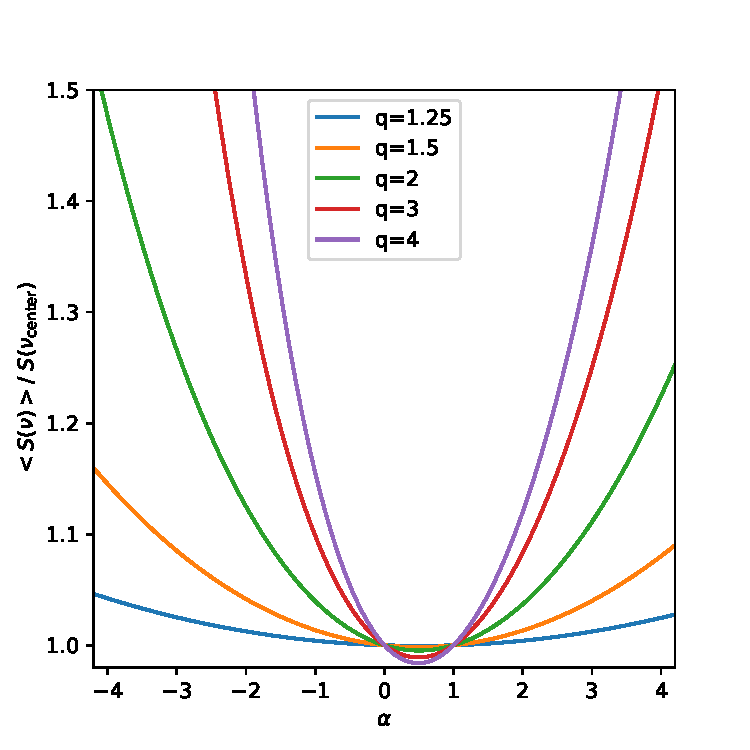
\includegraphics[width=1.0\textwidth]{figures/flux_bandcenter.pdf}\\
\caption[Spectral setup]{
	Ratio of the flux density averaged over the whole frequency coverage of the band (the measured flux density) and the flux density at the center of the band. The flux density is assumed to follow a power law. 
\label{fig:flux_bandcenter}}
\end{center}
 \end{figure}




%\begin{equation}
%	S_\nu\left(\nu\right) = S_\nu(\nu_0)\left[\frac{\nu}{\nu_0}\right]^\alpha
%\end{equation}

% We measure the flux density of this source from a band with an initial and final frequencies $\nu_0$ and $\nu_f$. The flux at the central frequency $\nu_c$ of the band is:
% 
% \begin{equation}
% 	%S_{\nu,{\mathrm{center}}} = 
% 	% S_\nu\left(\frac{\nu_f+\nu_0}{2}\right) = S_0\left[\frac{1}{\nu_0}\frac{\nu_f+\nu_0}{2}\right]^\alpha
% 	S_\nu\left(\nu_c\right) = S_0\left(\nu_0\right)\left[\frac{\nu_f+\nu_0}{2\nu_0}\right]^\alpha
% \end{equation}




\cleardoublepage
\phantomsection
\cleardoublepage
\phantomsection
\addcontentsline{toc}{chapter}{\listfigurename}
\listoffigures

\cleardoublepage
\phantomsection
\addcontentsline{toc}{chapter}{\listtablename}
\listoftables

% \cleardoublepage
% \printglossary[title=Glossary, toctitle=Glossary]
% \glsaddall
%\printglossary[title=Special Terms, toctitle=List of terms]


\bibliography{bibliography}

\cleardoublepage
\layout

\end{document}
